\documentclass{swfuthesism}

% 参照教程自己去写一个.bib文件
\addbibresource{ref.bib}   % 参考文献
\addbibresource{paper.bib} % publication

\swfusetup{
  Title={怎样用LaTeX撰写硕士毕业论文},%
  enTitle={How to write your MSc dissertation with LaTeX},%题目英文
  Author={某某某},%作者姓名
  enAuthor={Whoever},%作者姓名英文
  AuthorId={3.14159265},%学号
  Advisor={如雷贯耳},%指导教师
  enAdvisor={You Know Who (Professor)},%指导教师英文
  AdvisorTitle={教授},%指导教师职称
  ClsID={TP3.1415},%分类号
  Month=\the\month, Year=\the\year,%月、年
  DateA={2022/12/26},%提交论文日期
  DateB={2022/12/19},%论文答辩日期
  DateC={3},%独创性声明页上的日期
  Subject={很专业},%学科专业
  enSubject={Whatever},%学科专业英文
  Chairman={久仰久仰},%答辩委员会主席
}

\begin{document}

\maketitle

\begin{abstract} % 摘要
  本文是关于……
\end{abstract}

\begin{keyword} % 关键词
  关键词,关键词,关键词……
\end{keyword}

\begin{eabstract} % 英文摘要
  This project is about...
\end{eabstract}

\begin{ekeyword} % 英文关键词
  keyword, keyword, keyword...
\end{ekeyword}

\frontmatter
\tableofcontents % 目录
% \listoffigures % 插图目录,可以没有
% \listoftables  % 表格目录,可以没有

\cleardoublepage % keep this line

\mainmatter

% 参考教程,在chapters目录中单独写各章
\chapter{工欲善其事,必先利其器}
\label{cha:pre-requisite}

用\LaTeX{}撰写毕业论文是一件赏心乐事,前提是你得会。网上关于\LaTeX{}的入门教程很多,下面这
几个就很不错,花一两天时间去熟悉一下,

\begin{enumerate}
\item \LaTeX{} on Wikibooks\footnote{\url{https://en.wikibooks.org/wiki/LaTeX}}
\item The very short guide to typesetting with
  \LaTeX{}\footnote{\url{http://tug.ctan.org/info/latex-veryshortguide/veryshortguide.pdf}}
\item The not so Short Introduction to
  \LaTeX{}\footnote{\url{https://www.ctan.org/tex-archive/info/lshort/english/?lang=en}}
\end{enumerate}
有了对\LaTeX{}的基础认识之后,再接着往下看。

\section{工作环境}
\label{sec:env}

工作环境当然要清静、优雅。一杯热咖啡,配上轻音乐……除此之外,你还需要一
台电脑,最好是像我用的电脑。硬件不用太高级,但内存最好大一些,不少
于4G为宜,因为在我看,CPU已经足够快了,电脑运行是否顺畅,更多的是取决于
内存是否充足。下面简单介绍一下我们需要的软件环境和工具。

\subsection{操作系统}

我用Debian GNU/Linux ()%
\footnote{: \url{https://en.wikipedia.org/wiki/Debian}}的测试
(testing)版。为什么不用MS Windows? 因为~\ldots 当然不是它不好,而是我缺乏
足够的耐心。我的Debian系统从来不考验我的耐心。
很久以前,好像是2017年,在\href{https://www.zhihu.com}{知乎}上曾经看到
过一个问题 --- 不做开发的话,Linux是否适合日常使用?看到这个问题,我的第
一反应就是,“日常使用”这个词太含糊了。随后,我又意识到,如果认为“日常使
用”这个词不够具体,那么我就是在或多或少地承认“Linux不适合所有的日用场
景”。做为一个Debian铁杆用户,忽然发现“Linux不适合所有的日用场景”,这实
在令我有点沮丧。没错,我从1998年开始接触Debian,之后我所有的办公、私人
电脑上都只有Debian这一个系统。而且,我不是开发者。虽然我的确有一个计算
机专业的硕士学历,但十几年来,除了“Hello, world!”之外,我几乎什么程序都
没写过。我之所以写“Hello, world!”也完全是出于最基础的教学需要。我在大学
里教《Linux应用基础》和《操作系统原理》,讲到开发的时候,好歹得举个简单
的例子嘛。一个教计算机的老师不搞开发,我知道,这很不……。但是,做为一个
懒人,我也有我懒的借口。在天朝搞开发、搞科研,在我看就是“恭喜发财!”。
如果没有经济上的困扰,我觉得把时间兑换成钞票是相当不划算的事情。所以,
当我不得不对人家坦白说“我在事业上一事无成”的时候,我通常会向人家展示一
下我寒暑假的骑行游记\footnote{https://cs6.swfu.edu.cn/~wx672/travelogs},%
以此证明我这些年也没白活。否则,后面的聊天……反正我不觉得尴尬,
尴尬的就是别人。不管怎么说,我就是一个地地道道的Linux日常使用者,而且不搞开发,
而且我的Debian能满足我几乎所有的日常需求。当然,我的日常需求也的确相当
简单(上网、听歌、看片、写讲义、做幻灯片……)。

那么,Linux到底能不能应付所有的“日常使用”场景?我觉得,能,但你很难用某
一个通用的(默认安装配置的)Linux系统来满足所有的场景。通常,你要对自己
的系统做有针对性的配置,从而让它能够满足你的特定日常使用需求。与此相对
比,MAC OSX基本上做到了用一个系统来满足所有的用户需求,无需“私人订制”,
这的确是它的优势所在。但“私人定制”的确也是个诱人的字眼,不是吗?

那么,哪个Linux品牌(发行版)最好用?严肃地说,都一样好用。不信?在十
台电脑上装十个牌子的Linux,放到你面前,你会发现的确都很好用,也很漂亮,
而且你分辨不出谁是谁。换句话说,做为普通用户,你不必关心“牌子”问题,因
为各品牌的不同之处不在于使用,而在于管理。Debian和Redhat的系统管理方
式(操作命令、配置文件的格式等等)是大不相同的。而“管理”是管理员的事情,
做为一个普通用户的确不需要去操心。如果你想成为一个管理员,你至少得先成
为一个熟练用户才行吧。

那么,如果我打定主意要用Linux了,我该装哪个牌子的系统?我觉得,你周围的
熟练用户都用什么牌子,你就跟着用什么牌子。很显然,这样你能最方便地获得
帮助。如果你周围没有熟练用户,那么我建议你用Debian,因为它稳定性
好,bug少,软件库最大,社区最大,管理(软件包的安装、卸载、升级)方式简
单。下面简单罗列一下我在Linux平台不能顺利完成的事情:

\begin{itemize}
\item \href{https://im.dingtalk.com}{Dingtalk的网页版}似乎永久性地进入
  了“系统维护中”,为此,我尝试了WINE\footnote{https://wiki.winehq.org/Debian},%
  也尝试了在Virtualbox虚拟机里装
  个Android-x86\footnote{https://www.android-x86.org/},%
  两个办法都行得通,但总感觉代价偏高。WINE和Virtualbox都很优秀,问题出
  在钉钉上,它不仅臃肿,而且buggy,我实在没心情伺候它。还好,折腾了一
  年多之后,钉钉终于有了Linux版,虽然还是很臃肿、很buggy,但总算能对付
  着用了。
  % 所以我目前的解决
  % 方案是:1)如果想借用电脑的实体键盘快速打字的话,我就用scrcpy%
  % \footnote{https://github.com/Genymobile/scrcpy};2)如果想在电脑与手
  % 机之间快速传输文件,我就用qrcp%
  % \footnote{https://github.com/claudiodangelis/qrcp}。
\item Linux平台没有原生的炒股软件,但通过WINE也还可以挺顺畅地应付。
\end{itemize}

除此之外,我的Debian就只剩下优点了。当然,对于一个传统的Windows用户,
他要面对的困扰远不止这么两条,比如说,

\begin{itemize}
\item 他习惯于使用MS-Office做事情(可以尝试Libreoffice,或者WPS)
\item 他要玩游戏(也许可以WINE)
\item 他要QQ
\item 他要微信
\item 他要……
\end{itemize}


总之,做为入门用户,而且被Windows/QQ/Wechat/Baidu/360用户群包围着
\footnote{腾讯已经发布了QQ和微信的Linux版本,据说还不错。},又生
活在防火长城之下……困难总会有的,但并非无法克服。Debian可能是我人生中最
正确的一个选择了,干净,自由。

\subsection{桌面环境}

Linux社区流传着一句古老的元旦玩笑 --- “今年将是the year of Linux
desktop”。为了这一梦想,Linux的各个品牌都热衷于以华丽的桌面环境为诱饵,
招揽Windows用户。兄弟我年轻的时候,也是“重色思倾国”,和各种花容月貌的桌
面环境迷醉缠绵。后来发现,的确都很漂亮,但漂亮的东西都不便宜。一套完整
的Gnome或者KDE要安装数百个大大小小的软件包,占用数百兆硬盘,数百兆内存,
为系统增加数不清的bug,每次系统更新都要占用更多的带宽,花费更长的时间……而
这一切代价,只是为了“漂亮”和“方便”。

“漂亮”和“方便”当然是好事情,但它们是两个相当主观的词。“漂亮”很主观,情
人眼里出西施,母猪也能赛貂蝉,漂亮不漂亮的,基本上取决于你当时荷尔蒙的
高低,高兴就好。“方便”也很主观,我们身边的绝大多数电脑用户都是离不开鼠标的,因为它方便。但Emacs%
\footnote{: \url{https://www.gnu.org/software/emacs/}}或者Vim%
\footnote{: \url{https://www.vim.org/}}的粉丝们基本上完全抛开了鼠标,这
也是因为方便。对于Windows用户,抛开鼠标就像病人抛开拐杖一样痛苦。但只有
不依赖于拐杖的人才是健康的,不是吗?所以,怎么才算是方便呢,作为计科专
业的学生,你不该斟酌一下吗?

写毕业论文的话,我们完全不需要昂贵的桌面环境,有个便宜的window
manager就足够了。前面刚忏悔过,年轻的我是个desktop-hopper,在眼花
缭乱的桌面环境间换来跳去。“十年一觉扬州梦”,如今眼睛也花了,胡子也白
了,“再回首,……,才知道平平淡淡从从容容才是真”,于是
我返璞归真,由 desktop-hopper 变异为 WM-hopper。先用了十多年Sawfish%
\footnote{\url{https://en.wikipedia.org/wiki/Sawfish_(window_manager)}}
,Sawfish曾经是Gnome默认的窗口管理器,它界面足够的简单,功能足够的丰富,
配置足够的容易。而且和Emacs一样,它也是用Lisp写成的,算是Emacs的近亲吧。
这是我偏爱Sawfish的一个重要原因。后来,Sawfish老不更新,我就见异思迁,
另觅新欢,找了yet another Lisp-based tiling window manager ---
stumpwm\footnote{\url{https://stumpwm.github.io/}}。一直想好好学学Lisp,
无奈拖延症晚期了……又一变异,就躺平了。

近两年我都在用DWM\footnote{\url{https://dwm.suckless.org/}},一个很不
错的平铺式窗口管理器(tiling window manager%
\footnote{\url{https://en.wikipedia.org/wiki/Tiling_window_manager}})。%
它可以自动让所有的窗口互不重叠地铺满整个屏幕,非常适合大屏幕。%
而且dwm支持全键盘操作,有了它,你可以完全忘掉鼠标的存在。另外,作为一个
计科专业的学生,我觉得好歹你要做过一两个软件项目,才好意思写论文
吧。DWM就是个很小巧的C编程项目,代码量很少,易于学习。通过修改配置文件
就可以积累一些C编程的实战经验,何乐而不为?

\subsection{必备软件}

除了窗口管理器,显然你还需要几个“窗口”。下面这三个恐怕是必须有的:

\begin{description}
\item[Web浏览器] 原来我用Chromium\footnote{%
    : \url{https://en.wikipedia.org/wiki/Chromium_(web_browser)}},2019年
  初开始,改用Qutebrowser \footnote{%
    \qutebrowser{}: \url{https://en.wikipedia.org/wiki/Qutebrowser}} ,因为它小、快、灵、
  省内存、支持全键盘操作;
\item[PDF阅读工具] 我用Emacs的pdf-tools插件。在Emacs里,可以在一
  个buffer里写\TeX{},在另一个buffer里看PDF。还可以很方便地在两个buffer中
  对应的位置跳来跳去;
\item[终端] 我用st\footnote{\url{https://st.suckless.org/}}。其实,终端
  软件都差不多,有一个就行。真正不可或缺的
  是tmux\footnote{\url{https://en.wikipedia.org/wiki/Tmux}},有了它,一
  个终端可以当一万个用。
\end{description}

除了“窗口”之外,你还需要:
\begin{description}
\item[\LaTeX{}套件:]
  TeXLive\footnote{\url{https://en.wikipedia.org/wiki/TeX_Live}},它完
  备而庞大,但如果就是写个科技论文,我们只需要其中很少的一些软件包就够
  了。附录\ref{app:pkg}中列出了参照本教程写论文所需的所有软件包,可供参
  考。
\item[中文字体:] 完全不必操心,因为TeXLive有很好的中文支持。如果抛
  开\TeX{}不谈,就日常使用而言,我比较喜欢Noto字体\footnote{%
    \url{https://en.wikipedia.org/wiki/Noto_fonts}}。它是Google推出的开
  源字体。Debian库里自带,装上就好。所谓“Noto”就是Notofu的意思,也就是
  说Noto字体的终极目标是消灭所有的豆腐块(缺字)。Noto有专门的CJK字体包,
  只是尚缺楷体。楷体我用Debian库里自带的arphic-ukai,它是台湾文鼎科技\footnote{%
    \url{https://en.wikipedia.org/wiki/Arphic_Technology}}推出的开源字
  体。你当然也可以选用Windows字体,只要从你的Windows系统里拷贝过来就行
  了。这也许是你人生中唯一需要Windows的时候。
\end{description}

\subsection{编辑器}
\label{sec:emacs}

Emacs()是世界上最强大的编辑器\cite{emacs},没有之一。作为计科专业的
学生,如果你不熟悉它的使用,怎么好意思写毕业论文呢?我从1997年开始接
触Emacs,至今已经27年了。我不是程序员,从来就不是,但是,I love Emacs!
1997年的时候,还没有你今天见到的这么多IDE\footnote{%
  集成开发环境(Integrated Development Environment)。},所以Emacs就是
当年最好的IDE。25年来,虽然我既没有搞开发,也没为Emacs贡献任何插件,但
我还是从Emacs获得了巨大的乐趣。直到今天,在我看,Emacs还是最好的IDE。不
信?我们先看看什么是IDE。一个IDE无非包括如下一些功能模块:一个编辑器,
一个编译器,一个调试器,和其他一些辅助功能,比如用鼠标拖控件。什么是最
好的IDE?那肯定是:
\begin{center}
  最好的IDE = 最好的编辑器 + 最好的编译器 + 最好的调试器
\end{center}
有哪个IDE做到这一点了吗?只有Emacs。Emacs可以很方便地调用世界上
最牛的编译器(gcc)和调试器(gdb)。也许你会说“Emacs不能拖控件啊”,
没错,但在我看,拖控件并不总是一个受人欢迎的功能,至少在系统编程的时候,
它毫无用处。

而且,从学习的角度来说,拖控件,也就是用鼠标编程,绝对是一个非常恶
劣的习惯,因为这根本就是在逃避学习。鼠标化的IDE隐藏了很多学生应该了
解的技术细节。鄙学院的绝大多数学生居然不知道C程序是要编译之后才能运行的,
他们以为写好了程序,只要按那个“感叹号”按钮就可以了。这就是“鼠标教
学”的成果。Emacs可以帮助你克服鼠标依赖,强迫你熟练地使用键盘。

更重要的是,Emacs不只是个IDE,它是个ICE(Integrated Computing
Environment,这名字是我刚编出来的)。Emacs的设计目标就是,你装了
个Unix或者Linux系统,不需要装任何其它软件,只要装一个Emacs就够了,它能
帮助你完成所有的任务。也就是说,除了编程,你还可以用它写论文、做幻灯片、
浏览网页、收发邮件、聊天、听歌、看照片、玩游戏……目前,好像除了直接
在Emacs里看电影还不行,其它的都实现了。Emacs如此大一统的设计目标显
然有违Unix的设计原则 --- Do one thing, and do it well。 但好在Emacs是模块化
的,它的每一个功能模块都绝对遵循Do one thing, and do it well原则。你不
需要的功能模块,可以不安装。另外,还是从学习的角度来说,Emacs的学习曲线貌
似比其他IDE要长不少,但是
\begin{itemize}
\item 你不必学习VC去写C/C++,
\item 不必学习eclipse去写Java,
\item 不必学习MS-Word去写报告、幻灯片,
\item 不必学习……
\end{itemize}
一句话,“Everything Emacs”,可以省下大量不必要的学习时间。人生苦短,何
必让你的生活被 VC/Eclipse/MS-Word 搞得头昏脑胀呢? 简单而强大,本就是计
科专业学生和非专业学生应有的不同 。

Emacs绝对强大,但方便与否就见仁见智了,因为“方便”是一个很主观的概
念。反正,作为一个27年的老用户,我肯定觉得方便。其他IDE太无聊了,那么花
哨而庞大的东西,却只适用于应用层编程。既不能用来写论文,又不能做幻灯片,
更不能用来听歌、玩游戏。生活也太没有乐趣了。

最后一点,Emacs还是一个巨大的开放社区,在这里你能结识到更酷的程序
员。Emacs入门还是很简单的,它自带了一个基础教程。打开Emacs,按
\Ctrlh{t},教程就出现在你面前了。照着它边看边练,英文不太困难的话,一个小时应
该可以走完一遍了。针对写论文的话,你需要如下几个Emacs的插件:

\begin{itemize}
\item \auctex\footnote{\url{https://en.wikipedia.org/wiki/AUCTeX}}%
  是一个历史悠久、功能强大的Emacs插件,它为我们编辑\LaTeX{}文件提供了丰
  富的快捷键操作\cite{auctex}。
\item
  Yasnippet\footnote{\url{https://www.emacswiki.org/emacs/Yasnippet}}%
  也是Emacs的插件,它的功用就是为{\LKeyTab}键施加魔法\cite{yasnippet}。
  有了它,期待奇迹出现的时候,你只要左手小指在{\LKeyTab}键上轻轻一
  按……当然,你得先学会写魔咒(snippets)才
  行\,\Frowny{}。\label{p:yasnippet}放松,snippets都是很简单的小东西,
  去看看\texttt{\char`~/.emacs.d/snippets/latex-mode/}目录里的东西,我
  担保你能无师自通。
\item pdf-tools\footnote{\url{https://github.com/politza/pdf-tools}},
  前面已经提过了。即使不写\TeX{},单纯地为了阅读PDF文件,pdf-tools也是
  目前我认为最好用的阅读器,因为除了阅读,还可以标注PDF。
\end{itemize}

简而言之,有了上面几个插件,Emacs就成了一个强大
的\LaTeX{}排版IDE(图~\ref{fig:screenshot})。有了它,写论文可以像领导
说套话一样顺滑流畅。

\begin{figure}[ht]
  \centering
    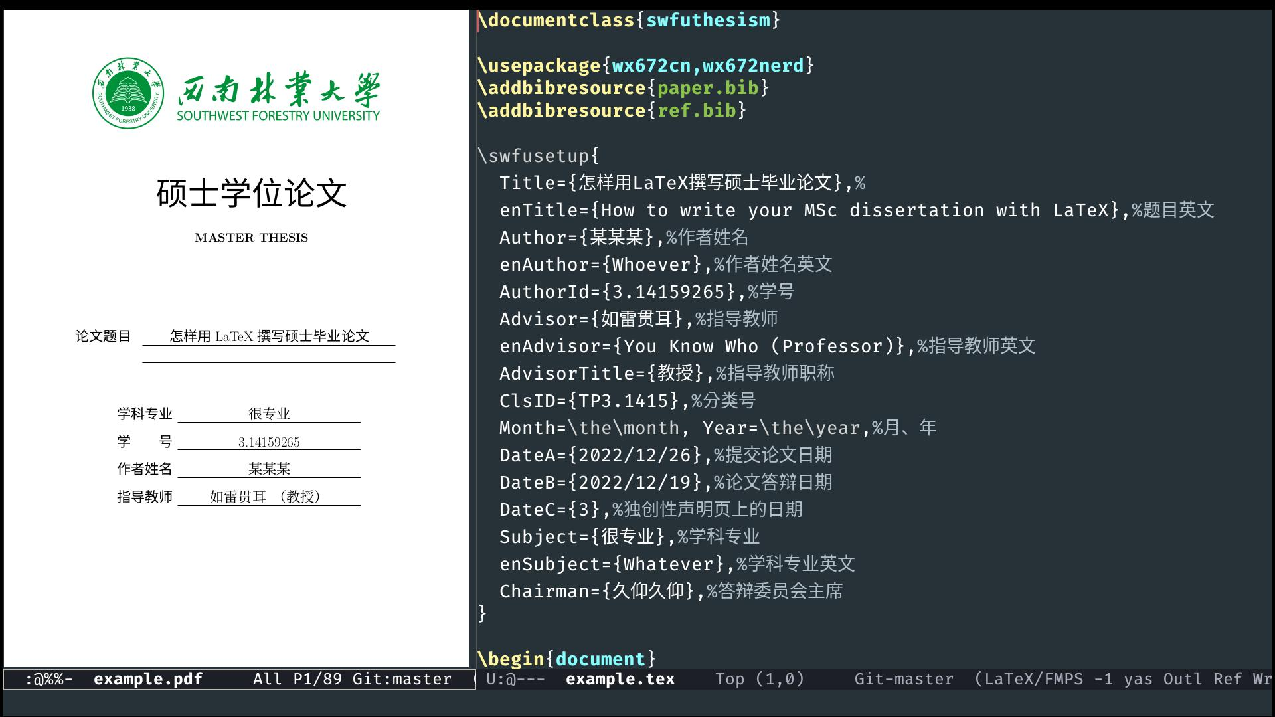
\includegraphics[width=.9\textwidth]{screenshot}
    \caption{在Emacs中编辑、预览论文\label{fig:screenshot}}  
\end{figure}

附录\ref{app:pkg}中列出了我的Debian系统上安装的与写论文相关的所有软件包,当然,清单里的
东西并非都是必需。其实,除了中文字体之外,其它的一切,你都可以根据自己的偏好来选择。如果你
打算用英文写论文的话,那么连中文字体都可以省略了。不管怎么说,上面提到的都是我个人的偏好,
本教程也将以此为基础,逐步展开。

至于如何安装、配置好这样一个工作环境,如果你是本校的学生,那么当然可以
直截找我帮忙。如果找不到我,那么你可以参考一下我曾经写过的一个简单的%
《Debian安装指导》\footnote{%
  \url{https://github.com/wx672/lecture-notes/blob/master/linux/tutorials/install/install.html}},应该能对你有点帮助的。

%%% Local Variables:
%%% mode: latex
%%% TeX-master: "../tutorial"
%%% End:

\chapter{快速上手}

\LaTeX{}很强大,但对于初学者来说,你不必关心它有多强大,因为最为常用的命令和环境不过寥寥数
个而已。而且Emacs \(+\) \auctex{}提供了丰富的快捷键,稍加练习之后,你就再也不用去手工敲命令了。
对于较复杂的格式需求,通常只要套用模版就可以解决问题了。所以,大家只要把Emacs用熟,
一切迎刃而解。

\section{用LaTeX写文章就是在编程}
\label{sec:hello}

\subsection{\texttt{hello.c}}
\label{sec:hello.c}

我们先回忆一下用Emacs写一个\texttt{hello.c}的键盘操作过程:

\begin{enumerate}
\item \Super{e},如果你的系统配置和我的一样,那么只要按下\Super{e}键,Emacs窗口就
  出现在你面前了,而且(感谢Sawfish)是全屏的;
\item \Ctrlxc{f},开始编辑一个新文件。这时,在Emacs窗口的最下面(也就是mini buffer里)有提
  示,输入你要编辑的文件的名字,也就是\texttt{hello.c},然后按\LKeyEnter{}(回车键),或者\Ctrl{j},其
  实,后面你会发现,\Ctrl{j}带自动缩进,比按\LKeyEnter{}更方便;
\item 现在可以在打开的空文件里写东西了:
  \begin{codeblock}[.7]
\begin{ccode}
#include <stdio.h>
int main()
{
  printf ("Hello, world!\n");
  return 0;
}
\end{ccode}
  \end{codeblock}
\item 存盘:\Ctrlxc{s}
\item 编译:\texttt{gcc hello.c}
\item 运行:\texttt{./a.out}
\end{enumerate}

\subsection{\texttt{hello.tex}}
\label{sec:hello.tex}

再看看用\LaTeX{}写一个\texttt{hello.tex}文件的过程:

\begin{enumerate}
\item \Super{e},打开Emacs;
\item \Ctrlxc{f},\texttt{hello.tex},开始编辑;
\item 写入文件内容:
  \begin{codeblock}[.7]
    \begin{latexcode}
\documentclass{article}
\begin{document}
Hello, world!
\end{document}
\end{latexcode}
  \end{codeblock}
\item 存盘:\Ctrlxc{s}
\item 编译:\texttt{xelatex hello.tex}
\item 看结果:\texttt{xpdf hello.pdf}
\end{enumerate}

怎么样? \texttt{hello.c}和\texttt{hello.tex}的编辑过程没什么分别吧。只要把Emacs用熟,触
类旁通,不管写什么程序,都是这么个过程。你
\begin{itemize}
\item 不必学习VC去写C/C++;
\item 不必学习eclipse去写Java;
\item 不必学习MS-Word去写报告、幻灯片;
\item 不必学习……
\end{itemize}
一句话,“Everything Emacs”,用程序员的方式做程序员的事情,你可以省下大量不必要的学习时间。
人生苦短,何必让你的生活被 VC/eclipse/MS-Word 搞得头昏脑胀呢? 简单而强大,就是计科专业和非
专业学生所应有的不同。如果你对Emacs操作还很陌生,那么现在就打开Emacs,\Ctrlh{t},重
温一下那些基本操作吧。

\subsection{什么是 \Ctrlxc{f}?}

% 「如果你爱他,逼着他用我的桌面环境;如果你恨他,逼着他用我的桌面环境。因为这里没有鼠标
% !」
使用Emacs是可以(而且应该)完全抛开鼠标的。对于初次上手的人,抛开鼠标就像病人抛开拐杖一
样痛苦。但只有不依赖拐杖的人才是健康的,不是吗?  
现在,你终于有了走向健康生活的冲动,那就开始吧。简短截说,
\begin{enumerate}
\item 先把你的双手在标准键盘上放好。然后,
\item 左手小指稍向左移,按在\LKeyCapsLock{}(CapsLock)键上\footnote{如果你的系统配置和我一
    样,那么\LKeyCapsLock{}就是\LKeyCtrl{}键。如果不是,那么你一定要想办法把它改成\LKeyCtrl{}键,因为在
    Emacs里\LKeyCtrl{}键实在是太常用了。},按住别放开,
\item 左手无名指稍向下移,在\LKey{x}键上轻按一下就放开,这就是\Ctrl{x};
\item 按在\LKeyCapsLock{}上的小指不要放开,左手食指在\LKey{f}键上轻按一下就放开,这就是\Ctrl{f};
\item 现在按在\LKeyCapsLock{}上的左手小指可以放开了。
\end{enumerate}
这就是\Ctrlxc{f},最常用的Emacs快捷键之一,作用是打开一个文
件\footnote{如果你要打开的文件不存在,那么Emacs会认为你要写一个新文件。},f代表file 。那么,
告诉我
\begin{itemize}
\item 什么是\Ctrlxc{s}?
\item 什么是\Ctrlx{2}? 什么是\Ctrlx{3}? 什么是\Ctrlx{o}? 什么
  是\Ctrlx{0}? 什么是\Ctrlx{1}?
\item 什么是\Ctrlx{h}? 什么是\Ctrl{w}?
\item 什么是\Ctrl{g}?
\item 什么是\Ctrl{j}? 什么是 \Ctrl{i}?
  % \item 什么是 \LKeyCtrlX{/}?
\item 什么是\Ctrl{k}? 什么是 \Ctrl{y}?
\item 什么是\Ctrl{d}? 什么是 \Meta{d}?
\item 什么是\Ctrl{a}? 什么是\Ctrl{e}? 什么是\Ctrl{f}? 什么是\Ctrl{b}? \\
  什么是\Ctrl{n}? 什么是\Ctrl{p}?
\end{itemize}

如果你还不熟悉上面这些快捷键,那么用起Emacs来,就会像西洋人用筷子一样不酷。「嘿!把你的手从
鼠标上拿开!」刚甩开拐杖,走向健康生活的人,总会不自觉地去扶点什么,这很正常。但你一定要坚
持锻炼,不要让这种「正常」持续得太久。今后的生活能否轻松愉快,主要就取决于你的健康程度。
如果有朝一日你真的抛开了鼠标,那么即使面对一个纯字符界面的终端,你也能写出漂亮的PDF格式的论
文。作为计科专业的学生,好歹该比网吧青年们酷一些嘛。

\section{生活可以更轻松}

\auctex{}是Emacs的一个功能模块,为\LaTeX{}编程提供了巨大的便利。有了它,你的\LaTeX{}生活可以
像\texttt{Hello, world!}一样简单。现在就跟着我,手把手地领略一下简单的乐趣吧。

一切当然是从\Super{e},打开Emacs开始。然后,\Ctrlxc{f},让我们开
始编辑一个新文件,就叫 \texttt{simple.tex}吧。

在Emacs窗口的最下方,也就是 mini buffer 里,这时应该会有提示,让你输入文件名。输
入\texttt{simple.tex}, 然后按 \Ctrl{j}。如果这时 mini buffer 里有如下提示:

\begin{itemize}
\item[] \texttt{Master file: (default this file) ...}
\end{itemize}

直接按 \Ctrl{j} 就可以了。知道了吧, \Ctrl{j} 就是我们的\LKeyEnter{}(回车)键。如果你的手正放在「标准
键盘」上,那么,左手小指向左一偏,按到的正是\LKeyCtrl{}键(\LKeyCapsLock{}{\scriptsize (CapsLock)}被我
们改造成\LKeyCtrl{}了)。右手食指下不正是\LKey{j}键吗?怎么样,比\LKeyEnter{}更方便吧。

现在,可以向 \texttt{simple.tex}文件里写东西了,\Ctrlcc{e},e代表environment。“环境”到底是什么
呢?意会吧,用用就明白了。在 mini buffer 里会有提示,

\begin{itemize}
\item[] \texttt{Environment type: (default document)}
\end{itemize}

这是在问你是不是要写一篇document(文章)啊?你当然该用\Ctrl{j}来告诉它「是」。这时,mini buffer 又会提示,

\begin{itemize}
\item[] \texttt{Document class: (default article)}
\end{itemize}

这是在问你是不是要写一篇 article 类型的文章啊?除了 article,通常还有 book, report, letter
可供选择。我们现在碰巧就是要写个短小的 article,所以,按\Ctrl{j}确认就好。这时, mini buffer 继续提示,

\begin{itemize}
\item[] \texttt{Options:}
\end{itemize}

这是在问你是否有什么特殊选项啊?用\Ctrl{j}来告诉它说「不需要」。现在,你的 \texttt{simple.tex}
文件里应该有如下几行东西了:
\begin{codeblock}[.9]
\begin{latexcode}
\documentclass{article}  % documentclass可以是
                         % article, book, report, letter...
\begin{document} % 文章的开始
| 
\end{document}   % 文章的结束
\end{latexcode}
\end{codeblock}
这时,光标停在 \verb|\begin{document}|与 \verb|\end{document}|之间,等待你的输入。百分号
(\verb|%|)后面显然都是注释。

在第\ref{sec:hello}节里,你已经会写 \texttt{Hello, world!}了。现在,我们要写点像模像样的东
西。偷懒起见,我直接套用Andrew Roberts 写的\texttt{simple.tex}\footnote{%
  \url{http://en.wikibooks.org/wiki/LaTeX/simple.tex}}。我们把注意力集中在用Emacs写文章的过
程上。

\subsection{Top matter}

先确保你的光标在 \verb|\begin{document}| 和 \verb|\end{document}| 之间,也就是文章的
第4行。然后按\Ctrlcc{m},这时 mini buffer 里会有如下提示:

\begin{itemize}
\item[] \verb|Macro (default ref): \|
\end{itemize}

这是系统在等待你输入一个 \texttt{Macro},说白了就是“命令”。输入:\texttt{title},\Ctrl{j},这时
你的文章会变成下面这样:

\begin{codeblock}[.9]
\begin{latexcode}
  \documentclass{article}  % documentclass可以是
                           % article, book, report, letter...
  \begin{document}         % 文章的开始
  \title{|} 
  \end{document}           % 文章的结束
\end{latexcode}
\end{codeblock}

这时,光标停在 \verb|\title{}| 的花括号里。不用说你也知道,该输入文章的标题了。那么就给它
一个标题:

\begin{codeblock}[.9]
\begin{latexcode}
  \documentclass{article}  % documentclass可以是
                           % article, book, report, letter...
  \begin{document} % 文章的开始
  \title{How to Structure a \LaTeX{} Document} 
  \end{document}   % 文章的结束
\end{latexcode}
\end{codeblock}
发现了吗?凡是以反斜杠开头的都是命令(\texttt{Macro}), 比如 \verb|\LaTeX{}|,它的唯一作用
就是把 \texttt{LaTeX} 这五个字母输出成一副怪样子,\LaTeX{}。

好了,在 title 下新起一行。然后\Ctrl{m}。你肯定知道 \Ctrl{m}是干什么用的了吧,就是要输入一
个 Macro。也许你会好奇,想知道总共有多少 Macro? 那么现在可以按一下\LKeyTab{}键。看到了吗?在弹
出的新窗口中,列出了近百个 Macro. 还好,我们并不需要记住这么多。最常用的也就三、五个而已。

mini buffer 里又会有提示:

\begin{itemize}
\item[] \verb|Macro (default title): \|
\end{itemize}

Emacs会把我们上次输入的Macro,也就是title,做为默认值提示出来。不用管它,输入:
\texttt{author} \Ctrl{j}。然后在 \verb|\author{}| 的花括号里输入作者的名字。当然,也可以把自己
的通信地址、email写在里面。就像下面这样:
\begin{codeblock}[.9]
\begin{latexcode}
  \documentclass{article}  % documentclass可以是
                           % article, book, report, letter...
  \begin{document}         % 文章的开始
  \title{How to Structure a \LaTeX{} Document}
  \author{Andrew Roberts\\
    School of Computing,\\
    University of Leeds,\\
    Leeds,\\
    United Kingdom,\\
    LS2 1HE\\
    \emph{andyr@comp.leeds.ac.uk}}
  \end{document}           % 文章的结束
\end{latexcode}
\end{codeblock}
注意,\verb|\\|代表“强制换行”。现在,新起一行,加上日期:

\begin{enumerate}
\item \Ctrlcc{m} date \Ctrl{j}
\item \Ctrlcc{m} today \Ctrl{j}
\end{enumerate}

其实,如果没有 \verb|\date{\today}| 这一句,系统会自动把今天的日期添加上的。而
且 \verb|\date{}|里面的日期你可以随意写,不一定非要是当天的日期。title, author, date 一般被
叫做文章的 top matter(开头那点事)。

再新起一行,写 \verb|\maketitle| \Ctrl{j}。\verb|\maketitle| 自然是要排版top matter了。换句
话说,不要标题的话可以省略掉这个命令。现在文章变成了这样:
\begin{codeblock}[.9]
\begin{latexcode}
  \documentclass{article}  % documentclass可以是
                           % article, book, report, letter...
  \begin{document}         % 文章的开始
  \title{How to Structure a \LaTeX{} Document}
  \author{Andrew Roberts\\
    School of Computing,\\
    University of Leeds,\\
    Leeds,\\
    United Kingdom,\\
    LS2 1HE\\
    \emph{andyr@comp.leeds.ac.uk}}
  \date{\today}
  \maketitle
  \end{document}           % 文章的结束
\end{latexcode}
\end{codeblock}
好奇的话,现在可以编译一下,看看PDF文件的效果:

\begin{enumerate}
\item 编译:\Ctrlcc{c}\quad\Ctrl{j}
\item 查看:\Ctrlcc{v}
\end{enumerate}

这时,一个PDF文件应该显示在屏幕上了(图\ref{fig:topmatter})。效果还满意吧?保持你的好奇心。在下面的操作中,你随时可
以编译一下看看效果。

\begin{figure}
  \centering
  \subcaptionbox{文章的起始部分\label{fig:topmatter}}{
    \fbox{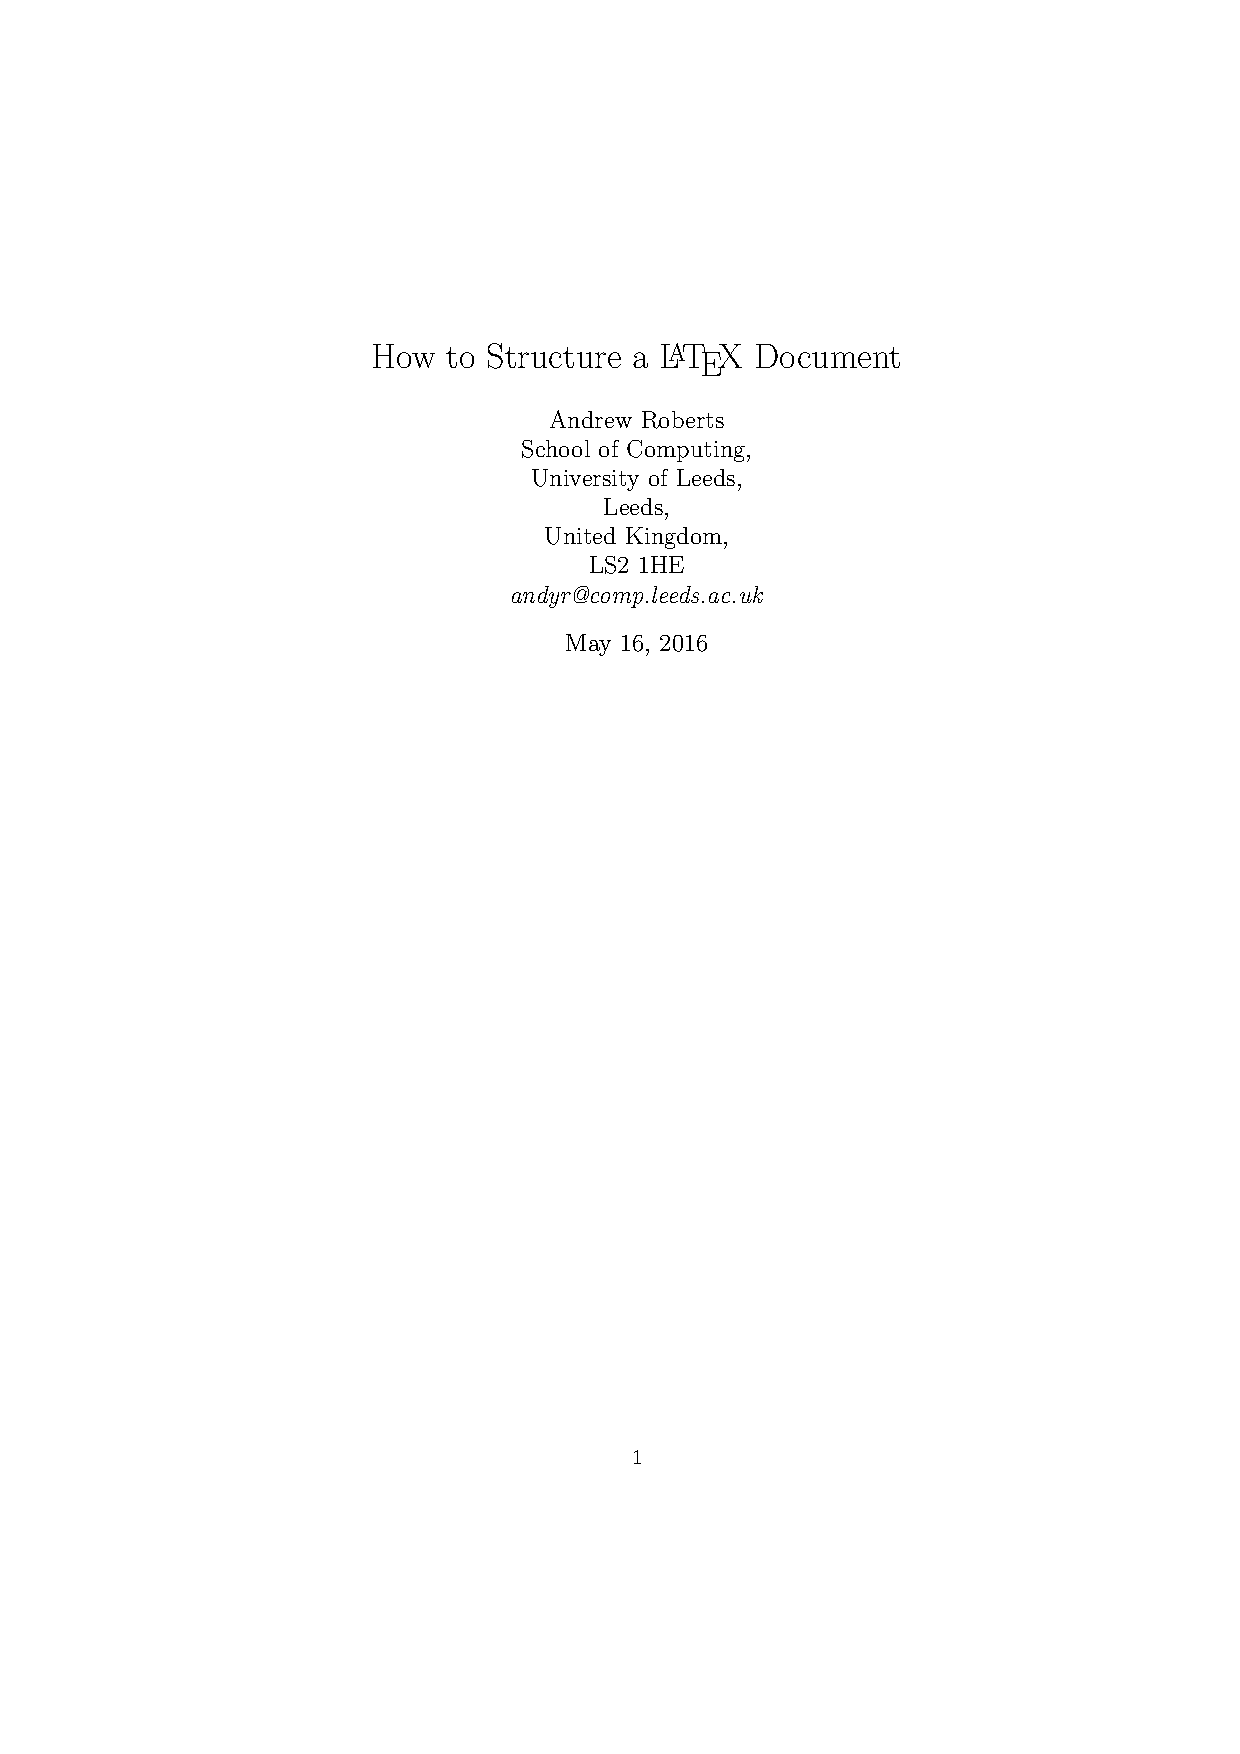
\includegraphics[width=.4\textwidth]{topmatter}}}\quad
  \subcaptionbox{加上摘要\label{fig:abstract}}{
    \fbox{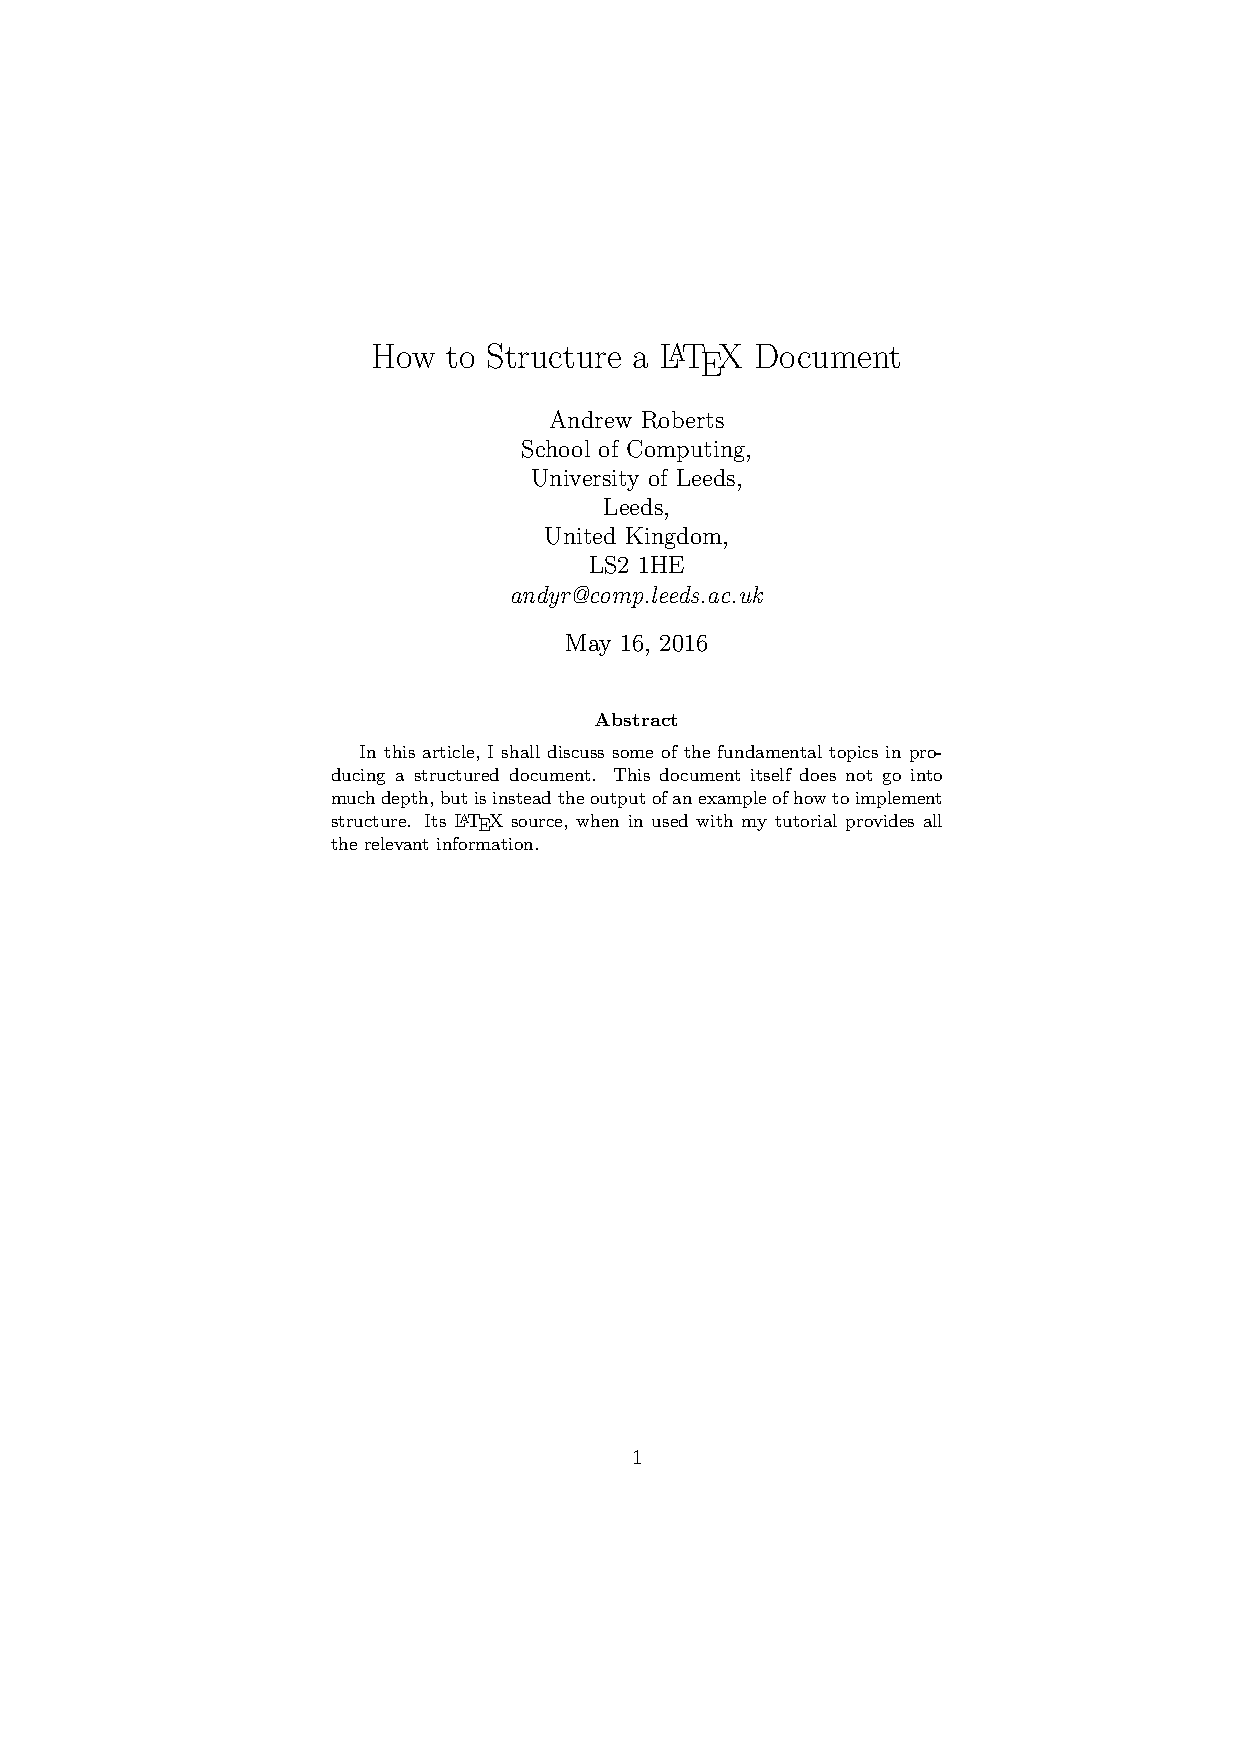
\includegraphics[width=.4\textwidth]{abstract}}}
  \caption{Top matter}
\end{figure}

\subsection{怎样写摘要}

好了,回到Emacs。现在你的光标应该停在 \verb|\maketitle| 的下面一行。我们开始写「摘要」部
分。\Ctrlcc{e},开始一个新的“环境”\footnote{如果你好奇心强,想知道总共有哪些“环境”的话,现在
  可以按{\LKeyTab}键。}。mini buffer 里提示:

\begin{itemize}
\item[] \texttt{Environment type: (default itemize)}
\end{itemize}

这是在问你要添加哪个环境啊?默认是最为常用的 itemize 环境。但我们现在要写的是“摘要”环境,
所以要告诉它:
abstract \Ctrl{j}。abstract 就是“摘要”的意思。科技论文都是要有摘要的嘛。于是,你的文章变成了这样:
\begin{codeblock}[.9]
\begin{latexcode}
  % 此处略去十数行
 
  \maketitle
 
  \begin{abstract} 
    |
  \end{abstract}
  \end{document}           % 文章的结束
\end{latexcode}
\end{codeblock}
光标停在 \verb|\begin{abstract}| 和 \verb|\end{abstract}| 之间(第6行)。好,现在往摘要部分里填点东西:
\begin{codeblock}[.9]
\begin{latexcode}
  % 此处略去十数行
 
  \maketitle
 
  \begin{abstract} 
    In this article, I shall discuss some of the fundamental
    topics in producing a structured document.  This
    document itself does not go into much depth, but is
    instead the output of an example of how to implement
    structure. Its \LaTeX{} source, when in used with
    my tutorial provides all the relevant information.
  \end{abstract}
  \end{document}           % 文章的结束
\end{latexcode}
\end{codeblock}
看看效果(图\ref{fig:abstract})。

\subsection{怎样分章节}

接着上面的例子,我们来写点更多更长的东西。偷懒起见,文章末尾
的 \ltx|\end{document}|我也不再写出来了。

好,按\Ctrl{n}把光标移到 \ltx|end{abstract}| 的下一行。然后,\Ctrlcc{s},让我们开始文章的第一节。
s 代表 section, “节”的意思。mini buffer 提示:

\begin{itemize}
\item[] \texttt{Level: (default section) }
\end{itemize}

显然是在问你,要不要起一个新 section 啊?没错,我就是要起一个新的章节,于是直接\Ctrl{j}。
mini buffer 又提示:

\begin{itemize}
\item[] \texttt{Title:}
\end{itemize}

也就是问你,章节标题是……?那就给它个标题吧,就叫“Introduction”。\Ctrl{j}之后, mini buffer 继续提示:

\begin{itemize}
\item[] \texttt{Label: sec:introduction}
\end{itemize}

这是在问你,要不要给这个新章节打个标签,比如 \texttt{sec:introduction}, 以后也许要索引到它呢?
这个暂时无关紧要,\Ctrl{j}就行了。于是,文中又有了下面的第5、6两行。
\begin{codeblock}[.9]
\begin{latexcode}
  % 此处略去十数行

  \end{abstract}

  \section{Introduction}
  \label{sec:introduction}
\end{latexcode}
\end{codeblock}
给这一节添加内容:
\begin{codeblock}[.9]
\begin{latexcode}
  % 此处略去十数行

  \end{abstract}

  \section{Introduction}
  \label{sec:introduction}

  This small document is designed to illustrate how easy
  it is to create a well structured document within
  \LaTeX\cite{lamport94}.  You should quickly be able to
  see how the article looks very professional, despite the
  content being far from academic.  Titles, section
  headings, justified text, text formatting etc., is all
  there, and you would be surprised when you see just how
  little markup was required to get this output.
\end{latexcode}
\end{codeblock}
注意到了吗?在这一节里有一个新命令 \verb|\cite{}|, 这是在引用一个参考文献。先不管它,后面再说。

如法炮制,再添加几个章节:
\begin{longlisting}
\begin{latexcode}
  % 此处略去十数行

  \end{abstract}

  \section{Introduction}
  \label{sec:introduction}

  This small document is designed to illustrate how easy
  it is to create a well structured document within
  \LaTeX\cite{lamport94}.  You should quickly be able to
  see how the article looks very professional, despite the
  content being far from academic.  Titles, section
  headings, justified text, text formatting etc., is all
  there, and you would be surprised when you see just how
  little markup was required to get this output.

  \section{Structure}
  \label{sec:structure}
  
  One of the great advantages of \LaTeX{} is that all it
  needs to know is the structure of a document, and then it
  will take care of the layout and presentation itself. So,
  here we shall begin looking at how exactly you tell
  \LaTeX{} what it needs to know about your document.
  
  \subsection{Top Matter}
  \label{sec:top-matter}
  
  The first thing you normally have is a title of the
  document, as well as information about the author and
  date of publication. In \LaTeX{} terms, this is all
  generally referred to as \emph{top matter}.

  |
\end{latexcode}
\end{longlisting}

注意到 \ltx|\emph{}| 了吗?它代表 emphasize ,“强调”。英文习惯用斜体字来表示强调的东西,那
么 \ltx|\emph{hello, world}| 自然就是把 hello, world 排版成 \emph{hello, world} 了。

注意到 \ltx|\subsection{}| 了吗?一会儿,我们还会看到 \ltx|\subsubsection{}|。不用解释吧,
文章的章节次序是这样:

\begin{minipage}{.9\linewidth}
  \begin{singlespace}
      \begin{tasks}(3)
      \task[] chapter
      \task[] section
      \task[] subsection
      \task[] subsubsection
      \task[] paragraph
      \task[] subparagraph
      \end{tasks}
  \end{singlespace}
\end{minipage}\par\vspace{2ex}

其中的chapter,只有在 book 和 report 中才能使用,而 article 只能用 section 以下的东西。

现在我们就来增加一个 subsubsection。不出所料的话,光标现在应该在第34行。那么
就\Ctrlcc{s},mini buffer 提示:

\begin{itemize}
\item[] \texttt{Level: (default subsection)}
\end{itemize}

当然输入:subsubsection \Ctrl{j}。mini buffer 提示:

\begin{itemize}
\item[] \texttt{Title:}
\end{itemize}

输入:Article Information \Ctrl{j}。mini buffer 提示:

\begin{itemize}
\item[] \texttt{Label: sec:article-information}
\end{itemize}

似曾相识吧?敲\Ctrl{j},于是,文章中又有了如下两行:
\begin{codeblock}[.9]
\begin{latexcode}
  \subsubsection{Article Information}
  \label{sec:article-information}
\end{latexcode}
\end{codeblock}
也就是说,我们有了一个 subsubsection。

\subsection{什么是环境}

现在,我们来添加一个 environment。\Ctrlcc{e},mini buffer 提示:

\begin{itemize}
\item[] \texttt{Environment type: (default abstract)}
\end{itemize}

我们当然不再需要 abstract 了,现在我们要的是 itemize ,也就是“不带序号的列表”。那么当然输
入:itemize \Ctrl{j}。于是看到:
\begin{codeblock}[.9]
\begin{latexcode}
  \begin{itemize}
  \item |
  \end{itemize}
\end{latexcode}
\end{codeblock}
光标停在 \ltx{\item} 的后面。非常好,这正是我想要的。于是直接输入如下文字:

\begin{itemize}
\item[] \ltx'\verb|\title{}|' --- The title of the article.
\end{itemize}

输入之后,\LKeyAlt{}+\LKeyEnter{},也就是,左手拇指按住\LKeyAlt{}键,同时右手小指去敲\LKeyEnter{}。你会看到
这样的效果:
\begin{codeblock}[.9]
\begin{latexcode}
  \begin{itemize}
  \item \verb|\title{}| --- The title of the article.
  \item 
  \end{itemize}
\end{latexcode}
\end{codeblock}
也就是说,不仅换了行,而且自动有了 \ltx{\item}等待你输入新的东西。

你一定注意到了 \ltx{\verb||} 这个新命令。它的作用和bash命令行的单引号 (\texttt{'}) 是一样的。
还记得吧,在命令行,单引号里的东西是原样输出的。 \ltx{\verb||} 里的东西也一样。 verb 是
verbatim 一词的缩写,就是“原样引用”的意思。好奇的话,可以编译一下,看看效果(图\ref{fig:env})。

\begin{figure}
  \centering
  \subcaptionbox{}{\fbox{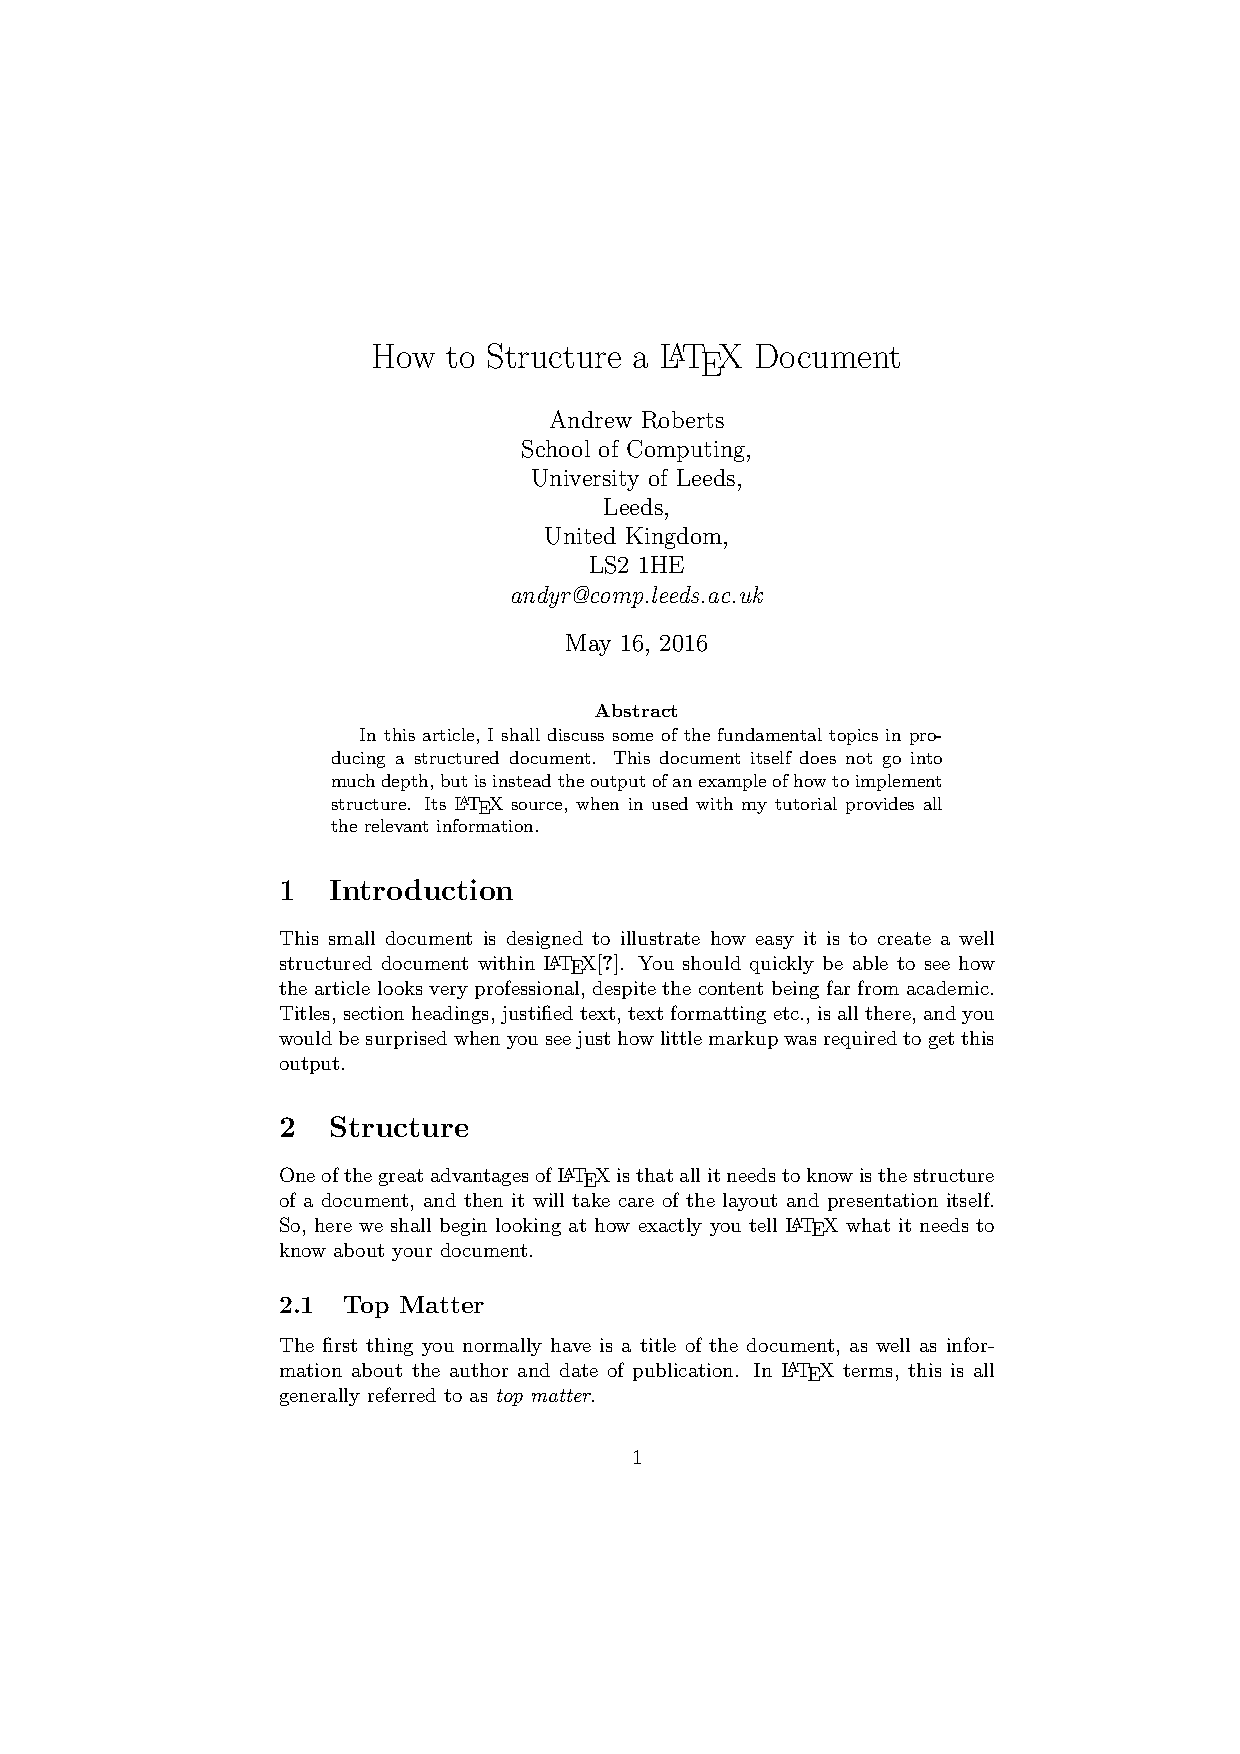
\includegraphics[width=.4\textwidth]{env1}}}\quad
  \subcaptionbox{}{\fbox{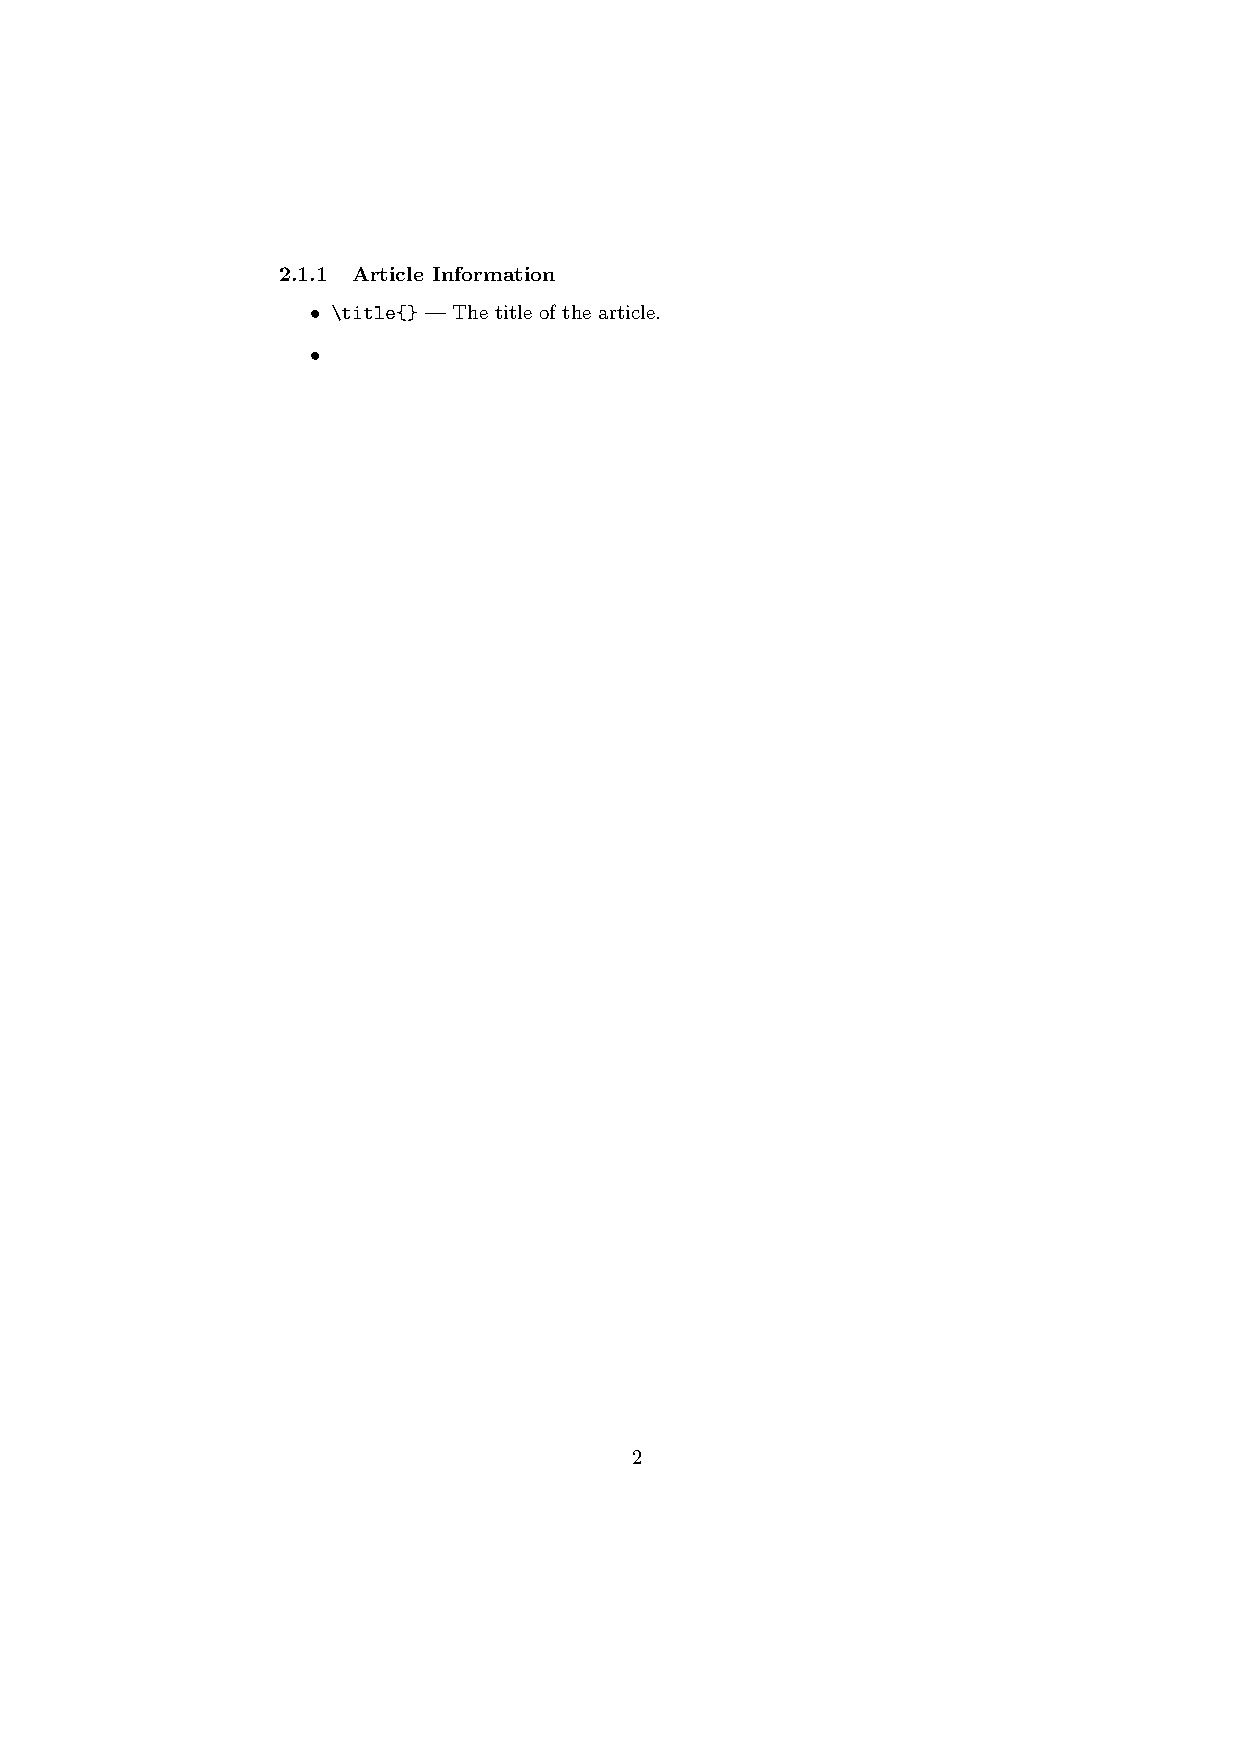
\includegraphics[width=.4\textwidth]{env2}}}
  \caption{输出效果\label{fig:env}}
\end{figure}

好,继续输入:

\begin{itemize}
\item[] \verb'\verb|\date| --- The date. Use:'
\end{itemize}

得到:
\begin{codeblock}[.9]
\begin{latexcode}
  \begin{itemize}
  \item \verb|\title{}| --- The title of the article.
  \item \verb|\date| --- The date. Use: 
  \end{itemize}
\end{latexcode}
\end{codeblock}
没什么好说的。现在我们要在 itemize 环境里面再套一个 itemize 。光标现在应该在第3行的最后。
敲:\Ctrlcc{e}\;\;\Ctrl{j},于是得到:

\begin{codeblock}[.9]
\begin{latexcode}
  \begin{itemize}
  \item \verb|\title{}| --- The title of the article.
  \item \verb|\date| --- The date. Use:
    \begin{itemize}
    \item 
    \end{itemize}

  \end{itemize}
\end{latexcode}
\end{codeblock}

简单吧?不用说了,你肯定知道下面这些是怎么来的了吧。

\begin{codeblock}[.9]
\begin{latexcode}
  \begin{itemize}
  \item \verb|\title{}| --- The title of the article.
  \item \verb|\date| --- The date. Use:
    \begin{itemize}
    \item \verb|\date{\today}| --- to get the date that
      the document is typeset.
    \item \verb|\date{}| --- for no date.
    \end{itemize}
  \end{itemize}
\end{latexcode}
\end{codeblock}

\begin{figure}
  \centering
  \fbox{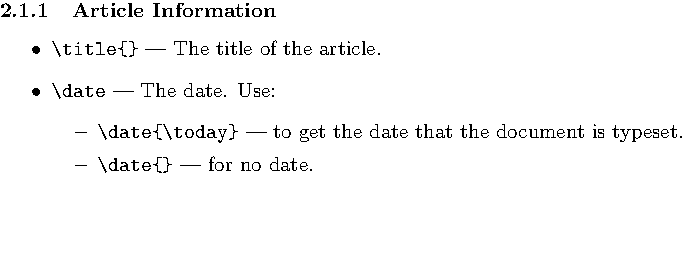
\includegraphics[width=.5\textwidth]{env3-crop}}
  \caption{itemize的输出效果\label{fig:itemize}}  
\end{figure}

编译之后的效果应该和图\ref{fig:itemize}差不多。
好了,请你现在照猫画虎,再来一个 subsubsection,标题叫 Author Information。模仿上面的东西,
来得到下面的东西:

\begin{codeblock}[.9]
\begin{latexcode}
  \subsubsection{Author Information}
  \label{sec:author-information}
  
  The basic article class only provides the one command:
  \begin{itemize}
  \item \verb|\author{}| --- The author of the document.
  \end{itemize}
  
  It is common to not only include the author name, but
  to insert new lines (\verb|\\|) after and add things
  such as address and email details.  For a slightly more
  logical approach, use the AMS article class (\emph{amsart})
  and you have the following extra commands:
  
  \begin{itemize}
  \item \texttt{address} --- The author's address.  Use the
    new line command (\verb|\\|) for line breaks.
  \item \texttt{thanks} --- Where you put any acknowledgments.
  \item \texttt{email} --- The author's email address.
  \item \texttt{urladdr} --- The URL for the author's web page.
  \end{itemize}
\end{latexcode}
\end{codeblock}

\begin{figure}
  \centering
  \fbox{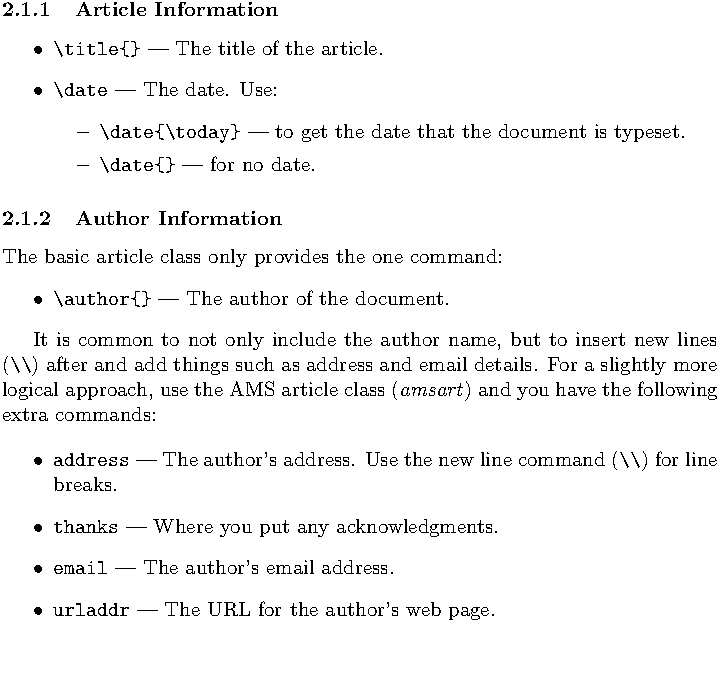
\includegraphics[width=.6\textwidth]{env4}}
  \caption{itemize的输出效果\label{fig:env4}}  
\end{figure}

显示效果如图\ref{fig:env4}所示。怎么样,不太困难吧? 目前为止,我们用到的无非是
表~\ref{tab:keys}中列出的这几个快捷键操作而已:

\begin{table}[!htbp]
  \centering\caption{常用快捷键\label{tab:keys}}  
  \begin{tblr}{colspec={rl},hline{1,2,Z}}
    快捷键&功用\\
    \Ctrl{j}&换行带缩进\\
    \Ctrlcc{m}&输入Macro\\
    \Ctrlcc{s}&新起一个章节\\
    \Ctrlcc{e}&新起一个环境\\
    \LKeyAlt{}+\LKeyEnter{}&换行带 \ltx{\item}\\
  \end{tblr}
\end{table}

好,趁热打铁,再起一个小节,

\begin{enumerate}
\item \Ctrlcc{s} subsection \Ctrl{j}
\item Sectioning Commands \Ctrl{j}\Ctrl{j}
\end{enumerate}

再添加一些文字,得到:
\begin{codeblock}[.9]
\begin{latexcode}
  % 此处略去数十行
 
  \subsection{Sectioning Commands}
  \label{sec:sectioning-commands}
  
  The commands for inserting sections are fairly intuitive.
  Of course, certain commands are appropriate to different
  document classes. For example, a book has chapters but a
  article doesn't.
  
  % A simple table. The center environment is first set up,
  % otherwise the table is left aligned.  The tabular
  % environment is what tells Latex that the data within
  % is data for the table.
\end{latexcode}
\end{codeblock}

% 再看看效果:
% \begin{center}
%   \fbox{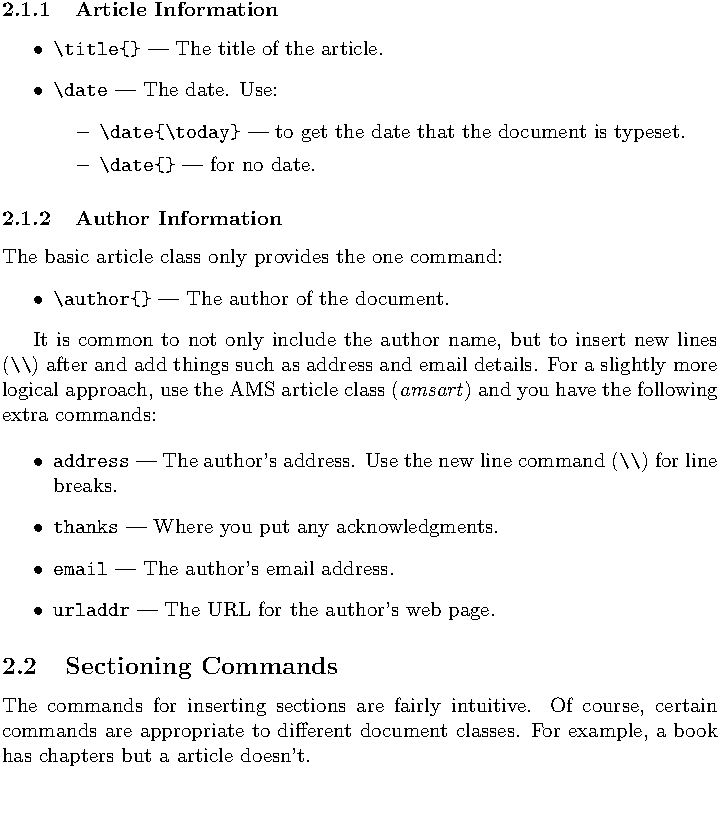
\includegraphics[width=.5\textwidth]{env5}}
% \end{center}
没什么新鲜东西,就不看效果了。下面抓紧说说怎么画表格。

\subsection{制作表格}

在这一小节,我们来尝试一下表格的输入。先起一个新“环境”,center,自然是“居中”的意思 :

\begin{enumerate}
\item[] \Ctrlcc{e} center \Ctrl{j}
\end{enumerate}

得到:

\begin{codeblock}[.9]
\begin{latexcode}
  % 此处略去数十行
 
  \subsection{Sectioning Commands}
  \label{sec:sectioning-commands}
  
  The commands for inserting sections are fairly intuitive.
  Of course, certain commands are appropriate to different
  document classes. For example, a book has chapters but a
  article doesn't.
  
  % A simple table. The center environment is first set up,
  % otherwise the table is left aligned.  The tabular
  % environment is what tells Latex that the data within is
  % data for the table.

  \begin{center}
    
  \end{center}
\end{latexcode}
\end{codeblock}

在center环境里面,我们添加一个 tabular(表格)环境:

\begin{enumerate}
\item[] \Ctrlcc{e} tabular \Ctrl{j}
\end{enumerate}

这时你会看到这样的提示:

\begin{enumerate}
\item[] \texttt{(Optional) Position:}
\end{enumerate}

Optional是可有可无的意思,也就是说,你如果在意表格的位置(Position),那么就提供位置信息;
如果不在意,那么就不用管它。现在我们连「位置」意味着什么都不清楚,自然就不必管它了。直接 \Ctrl{j},又看到提示了:

\begin{enumerate}
\item[] \texttt{Format:}
\end{enumerate}

这是问你,表格的格式,比如该有几列?每列之间要不要有竖线分割?等等。我的答案是这样:

\begin{enumerate}
\item[] \texttt{|l|l|}
\end{enumerate}

也就是:竖线(|),小写L(l),竖线(|),小写L(l),竖线(|)。小写L代表 left,也就是“左对齐”的
意思。那么,你应该恍然大悟了,不就是……竖线-左对齐-竖线-左对齐-竖线嘛。那么,举一反三,除了
小写L,我们还会见到r(右对齐)和c(居中)。现在 \Ctrl{j},得到如下结果:

\begin{codeblock}[.9]
\begin{latexcode}
  % 此处略去数十行
 
  \subsection{Sectioning Commands}
  \label{sec:sectioning-commands}
  
  The commands for inserting sections are fairly intuitive.
  Of course, certain commands are appropriate to different
  document classes. For example, a book has chapters but a
  article doesn't.
  
  % A simple table. The center environment is first set up,
  % otherwise the table is left aligned.  The tabular
  % environment is what tells Latex that the data within is
  % data for the table.

  \begin{center}
    \begin{tabular}{|l|l|}
      &
    \end{tabular}
  \end{center}
\end{latexcode}
\end{codeblock}

现在我们开始画表格,先画一条横线:

\begin{enumerate}
\item[] \ltx{\hline} \Ctrl{j}
\end{enumerate}

所谓 \ltx{\hline} ,顾名思义,就是 horizontal line。画完横线,开始第一行,

\begin{enumerate}
\item[] \verb'Command & Level \\ \hline' \Ctrl{j}
\end{enumerate}

那个 \verb'&' 就是两列之间的分隔符,``\verb'\\'''我们见过,表示强制换行。照猫画虎,把所有的
行都加上,得到如下结果:

\begin{codeblock}[.9]
\begin{latexcode}
  % 此处略去数十行
 
  \begin{center}
    \begin{tabular}{ll}
      \hline 
      Command & Level \\ \hline
      \verb|\part{}| & -1 \\
      \verb|\chapter{}| & 0 \\
      \verb|\section{}| & 1 \\
      \verb|\subsection{}| & 2 \\
      \verb|\subsubsection{}| & 3 \\
      \verb|\paragraph{}| & 4 \\
      \verb|\subparagraph{}| & 5 \\
      \hline
    \end{tabular}
  \end{center}
\end{latexcode}
\end{codeblock}

\begin{table}
  \begin{singlespace}
    \centering\caption{章节层次}\label{tab:level}
    \begin{tabular}{ll}\hline
      Command & Level \\ \hline
      \verb|\part{}| & -1 \\
      \verb|\chapter{}| & 0 \\
      \verb|\section{}| & 1 \\
      \verb|\subsection{}| & 2 \\
      \verb|\subsubsection{}| & 3 \\
      \verb|\paragraph{}| & 4 \\
      \verb|\subparagraph{}| & 5 \\ \hline
    \end{tabular}
  \end{singlespace}
\end{table}

这张表格的效果如表\ref{tab:level}所示。好了,表格画完了。再添加点文字:

\begin{codeblock}[.9]
\begin{latexcode}
  % 此处略去数十行 
  \begin{center}
    \begin{tabular}{ll}
      \hline 
      Command & Level \\ \hline
      \verb|\part{}| & -1 \\
      \verb|\chapter{}| & 0 \\
      \verb|\section{}| & 1 \\
      \verb|\subsection{}| & 2 \\
      \verb|\subsubsection{}| & 3 \\
      \verb|\paragraph{}| & 4 \\
      \verb|\subparagraph{}| & 5 \\
      \hline
    \end{tabular}
  \end{center}

  Numbering of the sections is performed automatically by
  \LaTeX{}, so don't bother adding them explicitly, just
  insert the heading you want between the curly braces. If
  you don't want sections number, then add an asterisk (*)
  after the section command, but before the first curly
  brace, e.g., \verb|section*{A Title Without Numbers}|.
\end{latexcode}
\end{codeblock}

现在编译一下,看看效果:

\begin{center}
  \fbox{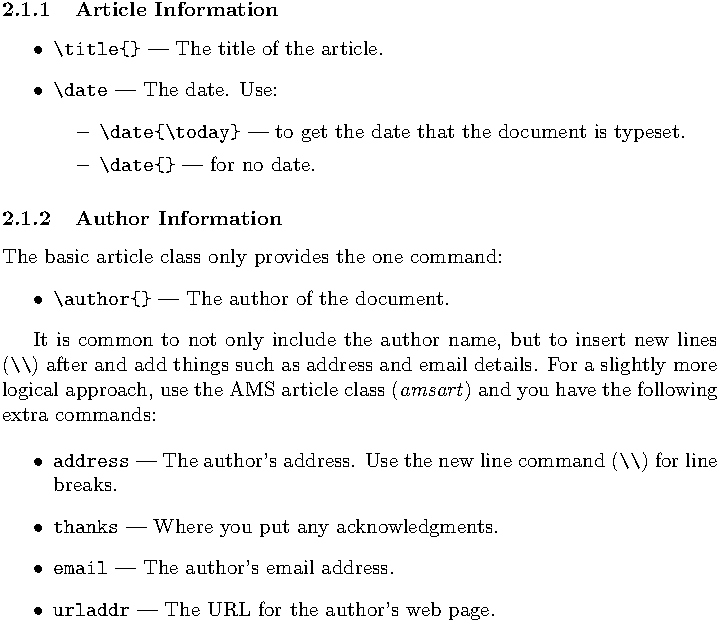
\includegraphics[width=.4\textwidth]{env6-crop-1}}
  \fbox{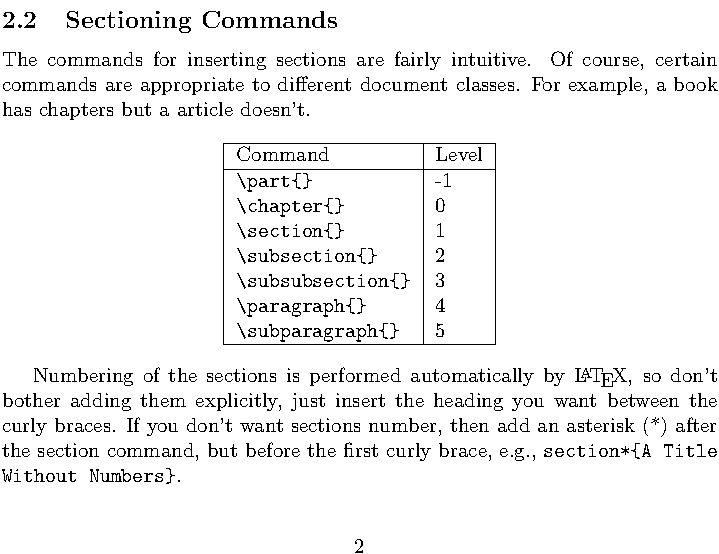
\includegraphics[width=.4\textwidth]{env6-crop-2}}
\end{center}

\subsection{引用参考文献}
\label{sec:ref}

处理参考文献,在\LaTeX{}中有两个选择:
\begin{itemize}
\item 传统的\bibtex{};
\item 时尚的\biblatex{}。
\end{itemize}
至于说两者的区别,粗略地说,\biblatex{}就是\bibtex{}的改进版。所以,下面我们只简要介绍一下
基于\biblatex{}的参考文献排版。

\subsubsection{第一步:准备好一个 \texttt{.bib} 文件}
Bib就是 Bibliography(参考文献)一词的前三个字母。顾名思义,在这个\texttt{.bib}文件里放的
都是你要用到的参考文献。我们这个小教程所用到的\texttt{tutorial.bib}文件就是个典型的例子。
节约篇幅起见,我们只列出该文件中的前三条记录如下:

\begin{longlisting}
\begin{bibtexcode}
@Misc{biblatex,
  author = {Philipp Lehman and Philip Kime and Audrey Boruvka and Joseph Wright},
  title = {The biblatex Package},
  month = 11,
  year = 2016}

@misc{ simple,
  author = "Andrew Roberts",
  title = "A simple article to illustrate document structure",
  year = 2003,
  url = "https://en.wikibooks.org/wiki/LaTeX/simple.tex",
}
@Book{Goossens94a,
  Title = {The LaTeX Companion},
  Author = {Michel Goossens and Frank Mittelbach and Alexander Samarin},
  Publisher = {Addison-Wesley},
  Year = 1994,
  Edition = {2nd revised},
}
\end{bibtexcode}
\end{longlisting}

怎么样,不难理解吧?照猫画虎地写出你自己的\texttt{.bib}文件应该不是件太困难的事情。

\subsubsection{第二步:引用参考文献}

准备好了你自己的\texttt{.bib}之后,剩下的事情就很简单了。简而言之,只要在你的\texttt{.tex}
文件里做三件事情……

首先,在\texttt{.tex}文件的\texttt{preamble}部分(也就是\ltx{\begin{document}}之前)加上如
  下一行(假设你的\texttt{.bib}文件名字是\texttt{myref.bib}):
\begin{codeblock}
  \begin{latexcode}
    \addbibresource{myref.bib}
  \end{latexcode}
\end{codeblock}

然后,在\texttt{.tex}文件中的适当地方,你要引用到你的参考文献(也就是\texttt{.bib}文件中
的相应条目)。举个例子:

\rule{.9\textwidth}{.4pt}\\[-5ex]
\singlespacing
\begin{minipage}[t]{.45\linewidth}
  \textbf{\latex:}
  \begin{minted}[fontsize=\small,
linenos=false,%numbersep=10pt,
frame=none,%framesep=3pt,rulecolor=\color{lightgray},
xleftmargin=0cm,%xrightmargin=4cm,
%gobble=4
]{latex}
在\biblatex{}手册中,作者说到,
\biblatex{}是对\latex{}的参考文献
处理模块的彻底改进\cite{biblatex}。
\end{minted}
\end{minipage}
\hfill\vline\hfill
\begin{minipage}[t]{.45\linewidth}
  \textbf{PDF:}\\[1.5ex]  
  在\biblatex{}手册中,作者说到,\biblatex{}是对\latex{}的参考文献处理模块的彻底改
  进\cite{biblatex}。
\end{minipage}
\begin{center}
\rule{0.9\textwidth}{.1pt}
\end{center}
\doublespacing

上例中的\ltx{\cite{biblatex}}就是要引用\texttt{myref.bib}中的第一条记录。在编译后输出的
PDF文件中我们会看到“\cite{biblatex}”。至于为什么是“6”而不是“1”或者其它什么数字,这取
决于生成参考文献时的排序选择,我们暂时不用关心它。

在\texttt{.tex}文件中要做的第三件事情是,在参考文献应该出现的地方加上如下一行:

\begin{codeblock}
\begin{latexcode}
\printbibliography{}
\end{latexcode}
\end{codeblock}

通常,“参考文献”应该作为一个章节出现在你的文章(或论文)的末尾。

\subsubsection{第三步:编译}

在上面的两步中,我们分别准备好了\texttt{.bib}和\texttt{.tex}文件,现在调用\texttt{latexmk}来编
译一下就行了。

前面我们都是用\texttt{xelatex}编译\texttt{.tex}文件,从来没提过\texttt{latexmk}。其实,不
用\texttt{latexmk}当然也可以完成文件的编译,具体步骤就是:
\vspace{-3ex}
\begin{singlespace}
  \begin{enumerate}
  \item \texttt{xelatex texfilename}
  \item \texttt{biber texfilename}
  \item \texttt{xelatex texfilename}
  \item 也许还要再执行一次上一行命令
  \end{enumerate}
\end{singlespace}
上面的第二步(调用\texttt{biber})就是用来处理参考文献的。如果觉得敲这三四个命令麻烦,那我
们就改用\texttt{latexmk}算了,唯一的前提条件是准备好一个小配置文件\texttt{.latexmkrc},内容
如下:
\begin{codeblock}[.9]
\begin{shellcode}
$pdf_mode = 1; $postscript_mode = $dvi_mode = 0;
$pdflatex = 'xelatex -interaction=nonstopmode -8bit --shell-escape %O %S';

$bibtex_use = 1;
$biber = 'biber --debug %O %S';
\end{shellcode}
\end{codeblock}

把这个小文件放到你自己的\verb|$HOME|目录下就行了。然后,只要:

\begin{codeblock}[.9]
  \begin{shellcode}
    latexmk texfilename
  \end{shellcode}
\end{codeblock}
不出错的话,一个带参考文献的PDF文件就诞生了。参考文献的样式就和本文的第\pageref{p:ref}页
差不多。

\section{小结}

本章我们借助于Andrew Roberts写的\texttt{simple.tex}文件,简要介绍了一下\LaTeX{}中最常用的命令和环境,同时
也熟悉了一些Emacs的基本键盘操作,在此做个小结。

\paragraph{最常用的命令}

\begin{tasks}(3)
\task[] \ltx{\title{}}
\task[] \ltx{\author{}}
\task[] \ltx{\date{}}
\task[] \ltx{\section{}}
\task[] \ltx{\subsection{}}
\task[] \ltx{\subsubsection{}}
\end{tasks}

\paragraph{最常用的环境}

\begin{tasks}(3)
\task[] \texttt{itemize}
\task[] \texttt{table}
\task[] \texttt{figure}
\task[] \texttt{enumerate}
\task[] \texttt{tabular}
\task[] \texttt{center}
\end{tasks}

\paragraph{最基本的Emacs快捷键(大多以\Ctrl{x}开头)}
\label{p:keys}

\subparagraph{文件操作}

\begin{tasks}(2)
\task[] 打开文件:\Ctrlx{f}
\task[] 存盘:\Ctrlx{s}
\task[] 关掉文件:\Ctrlx{k}
\end{tasks}

\subparagraph{编辑操作}

\begin{tasks}(2)
\task[] 终止命令:\Ctrl{g}
\task[] 缩进:\Ctrl{i}
\task[] 换行缩进:\Ctrl{j}
\task[] 剪切:\Ctrl{k}
\task[] 删除字符:\Ctrl{d}
\task[] 粘贴:\Ctrl{y}
\task[] 取消操作:\LKeyCtrl{}+\biolinumKeyGlyph{slash}
\task[] 设置标记:\LKeyCtrl{}+\LKeySpace{}
\end{tasks}

\subparagraph{移动光标}

\begin{tasks}(2)
\task[] 向前:\Ctrl{f}
\task[] 下一行:\Ctrl{n}
\task[] 向后:\Ctrl{b}
\task[] 上一行:\Ctrl{p}
\task[] 行首:\Ctrl{a}
\task[] 下一页:\Ctrl{v}
\task[] 行尾:\Ctrl{e}
\task[] 上一页:\Meta{v}
\end{tasks}

\subparagraph{窗口操作}
\begin{tasks}(2)
\task[] 横分:\Ctrlx{2}
\task[] 保留我:\Ctrlx{1}
\task[] 纵分:\Ctrlx{3}
\task[] 关掉我:\Ctrlx{0}
\task[] 切换:\Ctrlx{o}
\end{tasks}

\subparagraph{寻求帮助}

\begin{tasks}(2)
\task[] 教程:\Ctrlh{t}
\task[] info:\Ctrlh{i}
\task[] 函数:\Ctrlh{f}
\task[] 快捷键:\Ctrlh{k}
\task[] 变量:\Ctrlh{v}
\end{tasks}

\paragraph{最基本的\auctex{}快捷键(大多以\Ctrl{c}开头)}

\begin{tasks}(2)
\task[] 环境:\Ctrlcc{e}
\task[] 章节:\Ctrlcc{s}
\task[] 命令:\Ctrlcc{m}
\task[] 编译:\Ctrlcc{c}
\task[] 查看:\Ctrlcc{v}
\task[] \ltx{\item}:\LKeyAlt{}+\LKeyEnter
\end{tasks}

有了这些入门基础,我们已经可以应付要求不甚严格的文章排版了。但如果想排版出高质量的毕业论
文,hmm...,同志仍需努力。

在后续章节里,我们将简要介绍如下一些内容:

\begin{enumerate}
\item 如何插入图片
\item 如何写数学公式
\item 如何插入程序代码
\item 如何写中文
\item 如何使用毕业论文模版
% \item 如何做幻灯片
% \item Emacs org-mode
\end{enumerate}

%%% Local Variables:
%%% mode: latex
%%% TeX-master: "../tutorial"
%%% End:

\chapter{入门以后}

站在上一章的入门基础之上,本章我将介绍一些更为有趣的东西。这些貌似“高级”的技术其实也不复杂,
无非是再多认识几个命令和环境罢了。

\section{插入图片}

\begin{codeblock}[.9]
\begin{latexcode}
  \documentclass{article}
  
  \usepackage{graphicx}
  \graphicspath{{./figs/}{./}}
  
  \begin{document}
  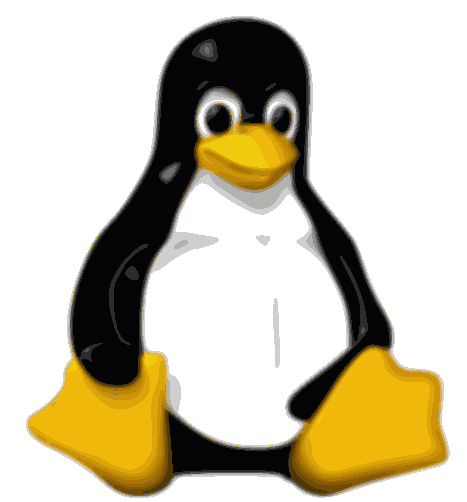
\includegraphics[width=5cm]{tux}
  \end{document}
\end{latexcode}
\end{codeblock}

怎么样,能看明白吗?插入图片用到了三个新命令:

\begin{enumerate}
\item \ltx{\usepackage{graphicx}}, 这是在说「我要用到一个名字叫 graphicx 的package(宏包)」。
  这很类似于我们C编程时常用的\cinline{#include<stdio.h>}。\ltx{\include-graphics{}}就
  是这个宏包提供的命令之一。想详细了解 graphicx的话,你可以打开一个命令终端,敲命
  令:\texttt{texdoc graphicx}。\texttt{texdoc}是TeXLive提供的专门用来看各种宏包手册的小工
  具。你可以通过\texttt{texdoc -h}命令来粗略了解它的用法。
\item \ltx{\graphicspath{{./figs/}{./}}}, 显然这是在指明graphics(图片)所在的path(路径,位
  置),也就是说,当你编译的时候,\LaTeX{}会到你指定的地方去找要插入的图片。在这里,我指定
  了两个地方:
  \begin{enumerate}
  \item \texttt{./figs/},当前目录下的\texttt{figs}目录。如果在这里没有找到,那么就去下面的
    目录里接着找;
  \item \texttt{./},也就是当前目录。如果在这个目录里还是没找到想插入的图片,那么编译器就要
    报错了。
  \end{enumerate}
\item \ltx{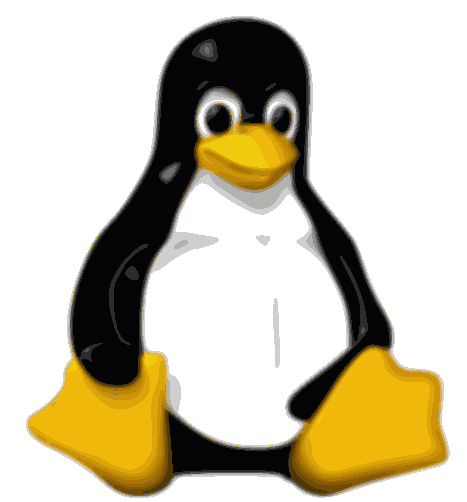
\includegraphics[width=5cm]{tux}},这显然就是在插入图片了。
  \begin{enumerate}
  \item 图片的名字叫 \texttt{tux.pdf}, 后缀(\texttt{.pdf})可以被省略掉。显
    然 \texttt{tux.pdf} 应该被存放在 \texttt{./} 或者 \texttt{./figs/} 中,才能被找到。我喜
    欢PDF图片,因为它可以自由缩放。你当然可以插入jpeg、png图片。
  \item 宽度是5cm,也可以是相对宽度,比如 \ltx{[width=.5\linewidth]} 就表示宽度等于0.5倍的行宽。
  \end{enumerate}
\end{enumerate}

如果你希望图片“居中”摆放,那自然是要用到 center 了:

\begin{codeblock}[.9]
\begin{latexcode}
  \documentclass{article}
  
  \usepackage{graphicx}
  \graphicspath{{./figs/}{./}}
  
  \begin{document}
  \begin{center}
    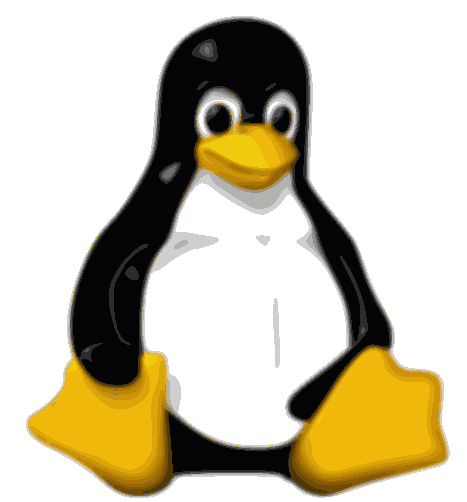
\includegraphics[width=5cm]{tux}
  \end{center}
  \end{document}
\end{latexcode}
\end{codeblock}

编译后的效果大致就是这样,居中,5cm宽。

\begin{center}
  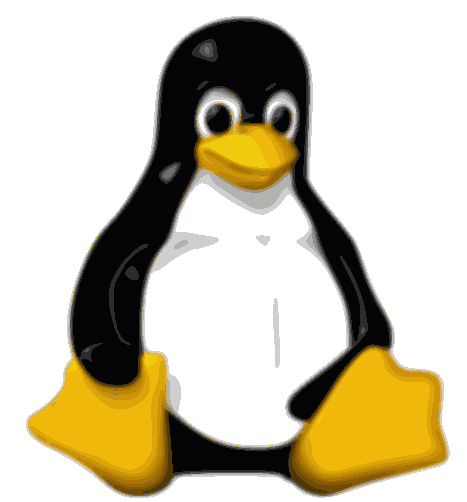
\includegraphics[width=5cm]{tux}
\end{center}

\subsection{Figure环境}
\label{sec:figure}

“哎,似乎应该加上图片说明吧?比如,【图1: Linux图标】?” 这个容易,只要用到一个新的
environment,叫figure。

\Ctrlcc{e} figure \Ctrl{j},mini buffer提示:
\begin{enumerate}
\item[] \texttt{(Optional) Float position:}
\end{enumerate}

这是在问你图片放在那里比较好啊?是靠上?还是靠下?还是懒得操心?如果没概念,那还是让LaTeX
来决定吧,\Ctrl{j}, mini buffer 提示:

\begin{enumerate}
\item[] \texttt{Caption:}
\end{enumerate}

这是在提示你输入图片的说明文字。那么输入:

\begin{enumerate}
\item[] \texttt{Linux logo}
\end{enumerate}

mini buffer 提示:

\begin{enumerate}
\item[] \texttt{Center? (y or n):} 
\end{enumerate}

当然选:

\begin{enumerate}
\item[] \texttt{y}
\end{enumerate}

mini buffer 提示:

\begin{enumerate}
\item[] \texttt{Label: fig:}
\end{enumerate}

这是要你给图片打个标签,以后方便索引到它。那么就给个标签:

\begin{enumerate}
\item[] \texttt{linux-logo}
\end{enumerate}

于是得到:

\begin{codeblock}[.9]
\begin{latexcode}
  \documentclass{article}
  
  \usepackage{graphicx}
  \graphicspath{{./figs/}{./}}
  
  \begin{document}
  \begin{figure}
    \centering
    
    \caption{Linux logo}
    \label{fig:linux-logo}
  \end{figure}
  \end{document}
\end{latexcode}
\end{codeblock}

现在你建立了一个完美的图片环境,别忘了把图片放进去。当然放在第9行:

\begin{codeblock}[.9]
\begin{latexcode}
  \documentclass{article}
  
  \usepackage{graphicx}
  \graphicspath{{./figs/}{./}}
  
  \begin{document}
  \begin{figure}
    \centering
    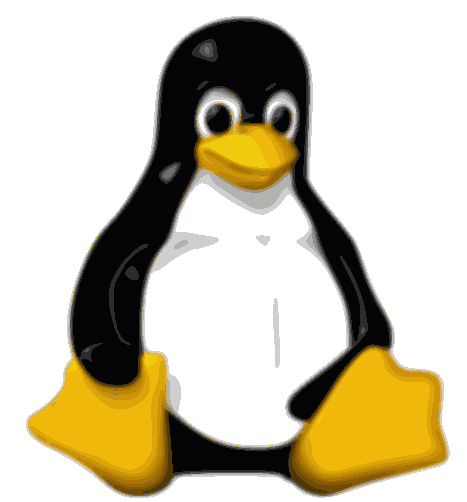
\includegraphics[width=5cm]{tux}
    \caption{Linux logo}
    \label{fig:linux-logo}
  \end{figure}
  \end{document}
\end{latexcode}
\end{codeblock}

编译后的效果如图\ref{fig:linux-logo}所示。

\subsection{\tbs{label\{\}}和 \tbs{ref\{\}}的用法}
\label{sec:label}

\ltx|\label{}|到底怎么用?来看下面的例子就明白了。

\begin{codeblock}[.9]
\begin{latexcode}
  \documentclass{article}
  
  \usepackage{graphicx}
  \graphicspath{{./figs/}{./}}
  
  \begin{document}
  \begin{figure}
    \centering
    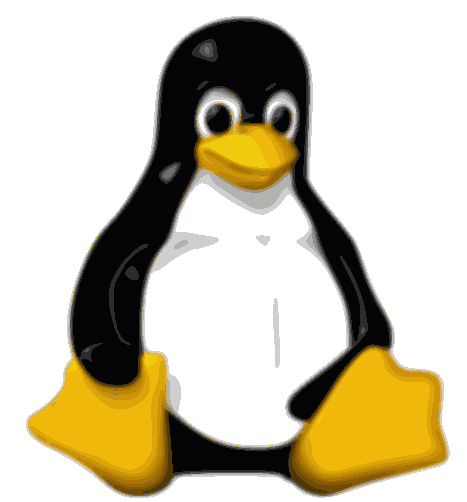
\includegraphics[width=5cm]{tux}
    \caption{Linux logo}
    \label{fig:linux-logo}
  \end{figure}

  Figure~\ref{fig:linux-logo} is the famous Linux Tux!
  图\ref{fig:linux-logo}所示就是大名鼎鼎的Linux吉祥物!
  \end{document}
\end{latexcode}
\end{codeblock}

编译一下,看看效果吧:

\begin{figure}
  \centering
  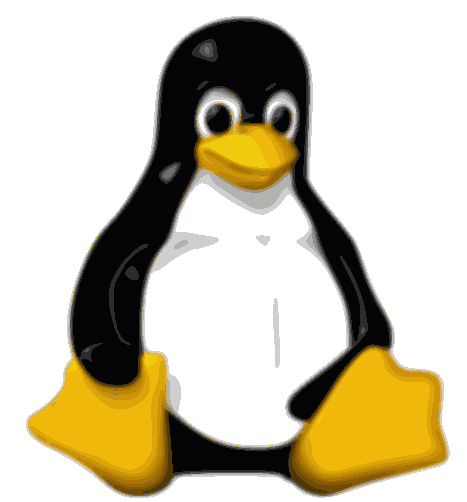
\includegraphics[width=5cm]{tux}
  \caption{Linux logo}
  \label{fig:linux-logo}
\end{figure}

\begin{center}
  \begin{minipage}{.6\linewidth}
    \hrule    \vskip 1ex
    Figure~\ref{fig:linux-logo} is the famous Linux Tux! 图\ref{fig:linux-logo}所示就是大名
    鼎鼎的Linux吉祥物!
    \vskip 1ex    \hrule
  \end{minipage}
\end{center}

\ltx{\label{}} 和 \ltx{\ref{}} 总是配合使用的,一个用来打标签,另一个用来找标签。而且这
两个命令可以被用在任何你需要的地方,非常方便。比如,

\begin{codeblock}[.9]
\begin{latexcode}
  % 本文的第一章标题
  \chapter{工欲善其事,必先利其器}
  \label{cha:pre-requisite}   % 章标签

  % 本文中的某张表格
  \begin{table}[!htbp]
    \centering
    \caption{常用快捷键}\label{tab:keys}  % 表格标签
    \begin{tabu*}to .5\textwidth {X[r]|X[l]}
      \hline
      \rowfont[c]{\bfseries}快捷键&功用\\\hline
      \Cj{}&换行带缩进\\
      \Cc\Cm{}&输入Macro\\
      \Cc\Cs{}&新起一个章节\\
      \Cc\Ce{}&新起一个环境\\
      \MEnter{}&换行带{\verb|\item|}\\\hline
    \end{tabu*}
  \end{table}

  % 在文中某处有这样一行
  最基本的Emacs快捷键(大多以\Cx{}开头)\label{p:keys} % 任意标签

  %%% 下面让我们来使用(索引)上面的标签
  
  \begin{enumerate}
  \item 本文的第~\ref{cha:pre-requisite}章介绍了一个简单、% 索引某章
    高效的工作环境;
  \item 在表~\ref{tab:keys}中列出了几个最常用的快捷键; % 索引某表
  \item 在第~\pageref{p:keys}页列出了更多的快捷键。    % 索引某页
  \end{enumerate}
\end{latexcode}
\end{codeblock}

上述代码就可以生成如下的效果,不仅数字是正确的,而且它们都是hyperlink,用鼠标点一下试试。

\begin{enumerate}
\item 本文的第\ref{cha:pre-requisite}章介绍了一个简单、高效的工作环境;
\item 在表\ref{tab:keys}中列出了几个最常用的快捷键;
\item 在第\pageref{p:keys}页列出了更多的快捷键。
\end{enumerate}

\subsubsection*{快捷地插入标签和索引}

插入标签和索引也是有快捷键的。\Ctrl{c}\biolinumKeyGlyph{braceleft}就是要插入标签,mini
buffer提示:

\begin{enumerate}
\item[] \texttt{Label: cha:}
\end{enumerate}

如果你不是要插入章标签,那么可以把\texttt{cha}改成其它你认为合适的字符。通常Emacs会根据光
标所在的环境给出不同的提示,如果光标在

\begin{itemize}
\item Figure里,它就提示\texttt{fig:};
\item Table里,它就提示\texttt{tab:};
\item 正文中其它什么地方,它就提示 \texttt{cha:}或者 \texttt{sec:}。
\end{itemize}

现在,在提示下输入一个简短而好记的标签名称,以便后面可以轻松找到它。

要插入索引(\ltx{\ref{}})的话,敲 \Ctrl{c}\biolinumKeyGlyph{braceright},mini buffer 提示:

\begin{itemize}
\item[] \texttt{SELECT A REFERENCE FORMAT}
\item[] \verb'[^M]  \ref'
\item[] \verb'[p]   \pageref' 
\end{itemize}

这是让你选择索引格式,如果想索引某页的话,就选\texttt{[p]}。其它任何情况,都选
择\verb'[^M]',也就是敲\LKeyEnter{}直接回车。根据你的选择,Emacs会弹出新的buffer,方便你找
到要引用的标签。

\section{数学公式}
\label{sec:math}

举个简单的例子吧:

\begin{codeblock}[.9]
\begin{latexcode}
  \documentclass{article}
  \begin{document}
  This is a simple math example: $c^2=a^2+b^2$
  \end{document}
\end{latexcode}
\end{codeblock}

结果是这样:

\begin{itemize}
\item[] This is a simple math example: $c^2=a^2+b^2$
\end{itemize}

美元符号(\verb'$')在 \LaTeX{}里面是特殊字符。夹在两个美元符号之间的东西,会被当做数学公式来排版。
如果想让数学公式独占一行的话,就用双美元符号(\verb'$$'),比如,
$$(1+x)^n=\sum_{k=0}^n\binom{n}{k}x^k$$
就是\verb'$$(1+x)^n=\sum_{k=0}^n\binom{n}{k}x^k$$'的输出结果。还不难看懂吧?

\begin{itemize}
\item \verb'\sum' $\Rightarrow\sum$
\item \verb'\binom{n}{k}' $\Rightarrow\binom{n}{k}$
\item 下划线(\texttt{\_})后面跟下标,如果下标不止一个字符,那么就要用花括号
  (\texttt{\{\}})括起来。比如,\verb'A_1 + A_{100}' $\Rightarrow{}A_1 + A_{100}$;
\item 上箭头(\verb'^')后面跟上标,用法和下划线一样。比如,\verb'2^2 \times 2^{32}'
  $\Rightarrow$ $2^2\times{}2^{32}$。 
\end{itemize}

那么,去哪里找这些数学符号呢?很简单,Google一下“latex math”,就什么都有了。“天啊,谁能记住
那么多数学符号啊?!”。\LaTeX{}的数学排版功能博大精深,各式各样的数学符号、怪异字符无所不及,
当然用不着都记住。你只要记住上面我们提到的几条,应该就足以应付毕业论文了。如果你要经常对付
复杂数学公式的话,那么最好把《The \LaTeX{} Companion》\cite{Goossens94a}这本书的第八章
(Higher Mathematics)打印下来放在手边,随用随查就好了。Google一下“latex math chapter 8”。

\section{插入程序代码}
\label{sec:code}

\begin{figure}
  \centering
\begin{minipage}[t]{.45\linewidth}
  代码:
  \begin{center}
    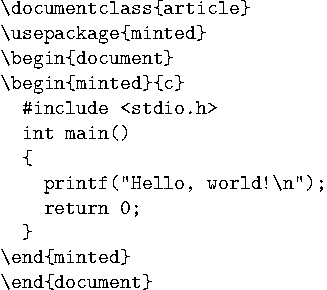
\includegraphics[width=\textwidth]{code}
  \end{center}
\end{minipage}
\hfill\vline\hfill
\begin{minipage}[t]{.45\linewidth}
  效果:
  \vspace{4.6em}
  \begin{minted}[baselinestretch=1,xleftmargin=0em]{c}
    #include <stdio.h>
    int main()
    {
      printf ("Hello, world!\n");
      return 0;
    }
  \end{minted}
\end{minipage}
  \caption{插入代码示例}\label{fig:code}
\end{figure}

还是从一个小例子开始吧,如图\ref{fig:code}所示,插入代码首先
要\ltx{\usepackage{minted}}。minted是用于美化代码排版的\LaTeX{}宏包,有了它,你可以把几乎
所有编程语言的代码排版得像你们老师那样道貌岸然,而且是彩色的。不过,对于毕业论文来说,还是
采用黑白排版比较好。彩色排版如果黑白打印,效果就很模糊了。当然你可以选择彩色打印,但那很费
钱啊。

想详细了解minted的用法,就:\texttt{texdoc minted}。minted宏包提供了一个新环境,就
叫minted ,把你的程序放在 \ltx|\begin{minted}|和\ltx|\end{minted}|之间就行
了。\ltx|\begin{minted}|后面的 \verb'{c}'当然是说,插入的程序是用C语言写的。
  
怎么?程序太长,拷贝进来太麻烦?那么可以这样:

\begin{codeblock}[.9]
\begin{latexcode}
  \documentclass{article}
  \usepackage{minted}
  \begin{document}
  
  \inputminted{c}{hello.c}
  
  \end{document}
\end{latexcode}
\end{codeblock}

简单吧?\texttt{hello.c} 当然要和你的 \TeX{} 文件在同一个目录下,否则你要指明详细路径。

minted宏包提供了丰富的命令,可以支持数十种编程语言,后台调用强大的pygments来打扮你的程序
代码,可以把程序以各种你能想到的方式排版出来。当然,使用 minted 的前提条件是,系统里已经安
装好了python和pygments。这一点在minted的手册里已经说得很清楚了。关于强大的pygments,
你该去它的网站看看:\url{http://pygments.org/}。

\section{处理中文}
\label{sec:cn}

如果你的Emacs配置和我的一样,那么输入中文就是“piece of cake”,当然你得安装了中文输入法,我
用的是fcitx\footnote{\url{https://fcitx-im.org/wiki/Fcitx}},挺好用的。

现在,打开一个全新的\texttt{tex}文件,比如\texttt{hello.tex},在里面写\texttt{ctexart},然
后敲\LKeyTab{}(TAB)键,一个现成的\LaTeX{}文件模板立时会展现在你的面前。这个模版里有你写一篇漂
亮中文文章所需要的一切。光标就停在 \ltx|\title{}| 的花括号里,那么就开始用中文填空
吧。重点就是第一句:

\begin{latexcode}
\documentclass[scheme=chinese]{ctexart}
\end{latexcode}

也就是说,只要直接采用\texttt{CTeX}提供的\texttt{ctexart class},中文问题就不需要我们操心
了。


%%% Local Variables:
%%% mode: latex
%%% TeX-master: "../example"
%%% End:

\chapter{完美的毕业论文}
\label{cha:thesis}

写毕业论文,像结婚一样,是一生一次的大事情。潦草而失败的论文,就像失败的婚姻,总要一次次地
返工,在痛苦中煎熬,直到你遇见ta,带你摆脱迷茫、痛苦,登上幸福的彼岸\footnote{我说的当然
  是\LaTeX{}。}。

\begin{itemize}
\item[] 写普通文章要用 \verb'\documentclass{article}';
\item[] 写报告要用 \verb'\documentclass{report}';
\item[] 写书要用 \verb'\documentclass{book}';
\item[] 写信要用 \verb'\documentclass{letter}';
\item[] 那么写毕业论文自然要用毕业论文模版了:\verb'\documentclass{swfuthesis}'。
\end{itemize}

如此关系人生的大事情,当然要为它专门建立一个目录吧。目录建好了,把论文模板 \texttt{swfuthesis.cls} 文件拷贝
进去。然后就可以用它来写你的论文了。

\section{Class文件}
\label{sec:class}

Class文件\footnote{也就是后缀为\texttt{.cls}的文件,也就是我们常说的模板文件。},它决定了你
的文章样式,比如说,纸张尺寸、页边距、行距、字距、字体、标题样式等等在class文件中都做了设
置。除此之外,我们在写\texttt{tex}文件的过程中用到的命令(Macro)也都是class文件提供的。

这里有一个值得注意的概念,排版这件事情,是由排版软件根据你(在文章中提供)的命令来进行的。
只要你的命令正确,文章的格式就必然是正确的。这就是排版软件和字处理软件(比如MS-Word)的区
别所在。利用字处理软件来写文章,你不得不既操心文章的内容,也操心文章的格式。而利用排版软件,
比如\LaTeX{}来写文章,你只需要关心文章的内容,而格式的事情,排版软件会根据你的命令来替你完
成。所以,你输入的命令必须正确、合法、合情理才行。

排版软件只能理解class文件中提供的命令\footnote{我说谎了,实际上,在\texttt{tex}文件中,你可
  以利
  用 \texttt{\textbackslash{}newcommand\{\}}和 \texttt{\textbackslash{}renewcommand\{\}}来
  定义自己的命令。但对于初学者来说,你暂时还不必操心这个,class文件所提供的命令应该足以应付
  你目前的需求了。},所以,我们当然要对这些命令有个基本的了解。附录\ref{app:class}中就
是\texttt{swfuthesis.cls}文件的全部内容。我们在此做个简要介绍。简而言
之,\texttt{swfuthesis.cls}提供了如下一些基本命令:
\begin{singlespace}
  \begin{multicols}{2}
    \begin{enumerate}
    \item \verb'\title{论文标题}'
    \item \verb'\author{作者}'
    \item \verb'\enTitle{论文标题}'
    \item \verb'\enAuthor{作者}'
    \item \verb'\Advisor{指导教师姓名}'
    \item \verb'\AdvisorTitle{指导教师职称}'
    \item \verb'\Month{这里填月份}'
    \item \verb'\Year{这里填年份}'
    \item \verb'\Subject{这里填专业}'
    \item \verb'\maketitle':用于生成封面
    \item \verb'\makebib':用于生成参考文献
    \end{enumerate}
  \end{multicols}
\end{singlespace}
和如下一些环境:
\begin{singlespace}
  \begin{multicols}{2}
    \begin{enumerate}
    \item \verb'abstract':中文摘要
    \item \verb'keyword':中文关键词
    \item \verb'EAbstract':英文摘要
    \item \verb'EKeyword':英文关键词
    \item \verb'advisorInfo':指导教师简介
    \item \verb'acknowledgment':致谢
    \end{enumerate}
  \end{multicols}
\end{singlespace}
\section{模板的使用}

具体如何使用这些命令呢?简而言之,\Cx\Cf{},输入一个崭新的文件名,\Cj{}。现在,面对空无一字
的Emacs窗口,你有生以来最重要的一篇文章就要开篇了,你在思考什么?其实什么都不用想,直接
敲 \texttt{thesis} {\Tab}(Tab),一个论文框架就呈现在你的眼前了,你要做的就是用你前面学到的
那些\LaTeX{}命令来填空。

在本文开始的时候(第\pageref{p:yasnippet}页),我们提到过“{\Tab}大法”是\texttt{yasnippet}的
贡献。所以,你在期待{\Tab}键能带来奇迹之前,必须先确保你的系统里已经装好了
\texttt{yasnippet}。如果还没装上,那么就执行下面的命令\cite{aptitude}:

\begin{codeblock}
  \begin{shellcode}
sudo apt update && sudo apt upgrade
sudo apt install yasnippet yasnippet-snippets
  \end{shellcode}
\end{codeblock}

装好之后,重新加载Emacs的配置文件。很简单,在Emacs窗口里,敲

\begin{itemize}
\item[] \Mx{} \texttt{load-file} \Cj{} \verb'~/.emacs' \Cj{}
\end{itemize}

跟着本教程写论文的前提条件就是,Emacs必须工作正常,如果发现问题必须及时处理,不能将就。尤其
是在入门阶段,不要指望用一个别扭的Emacs来顺畅地写出完美的论文。

附录\ref{app:thesis}中列出了完整的毕业论文框架,也就是你在键入\texttt{thesis} {\Tab}后应
该看到的东西。如果奇迹没有发生,那么就要操心一下你的Emacs配置了。

假设你的Emacs环境良好,按{\Tab}键之后,本来空荡荡的Emacs buffer里现在有了一个论文框架,而且
光标就停在你要填空的第一个位置,也就是 \verb'\title{论文标题}'的花括号里。这时,你只要键入
任何文字(通常应该是你自己的论文标题),(感谢\texttt{yasnippet})花括号里的“论文标题”四字
就会被自动替换掉。写好了论文标题,还是按{\Tab}键,光标会自动跳到下一个你需要填空的位置。如
此一直{\Tab}下去,直到光标不再跳开了,那就是你该写论文第一章内容的时候了。

论文框架里有足够多的注释,再加上你在前几章学到的本领,我相信写出一个规范、漂亮的毕业论文应该是手
到擒来的事情了。

\section{生成参考文献}

在第\ref{sec:ref}节中我们已经介绍过如何处理参考文献。大致步骤:
\begin{enumerate}
\item 准备好一个\texttt{.bib}文件(假设名字叫\texttt{myref.bib});
\item 在\texttt{.tex}文件中做三件事:
  \begin{enumerate}
  \item 在\texttt{preamble}中加一句 \verb|\addbibresource{myref.bib}|;
  \item 在正文中适当的地方利用\verb|\cite{}|命令引用\texttt{myref.bib}文件中的参考文献条目;
  \item 在文章的结尾部分加一句\verb|\printbibliography{}|;
  \end{enumerate}
\item 用\texttt{latexmk}来编译\texttt{.tex}文件.
\end{enumerate}

附录\ref{app:bib}中列出了本文所用到的\texttt{.bib}文件(\texttt{tutorial.bib})。
你可以对照着第\pageref{p:ref}页的参考文献部分看看,找找感觉。

\paragraph*{这个文件是怎么来的?}

当然可以手写。\texttt{bib}文件的格式清晰易懂,照猫画虎地手写并不困难。但生活可以更轻松,如
果你引用的书籍、资料不是太冷门,那么通常只要google一下「书名 bibtex」,就可以找到相应
的\texttt{bib}条目了。有时你甚至可以从网上下载到现成的bib文件,比如全
套RFC\footnote{Request for
  Comments. \url{https://en.wikipedia.org/wiki/Request_for_Comments}}的\texttt{bib}文件。

\paragraph*{怎样使用这个文件?}

很简单,三件事:

\begin{enumerate}
\item 第一件事不用做,因为在我们的论文模板文件(\texttt{swfuthesis.cls})里已经做了。在模板
  文件里有如下一行:\par            \hspace{4em}\verb|\RequirePackage[backend=biber,style=gb7714-2015]{biblatex}|\par
  也就是说,帮我们排版参考文献的是\texttt{biblatex}宏包;
\item 在\texttt{tex}文件(你的论文)的preamble部分,也就是在\verb|\begin{document}|之前,加
    上如下一行:\par\hspace{4em}\verb|\addbibresource{tutorial.bib}|\par
    很显然,这是在告诉\texttt{biblatex}从当前目录下的\texttt{tutorial.bib}文件里去读取参考
    文献信息。
  \item 这件事也不用做了,因为在论文的框架文件(\texttt{tex}文件)里已经做好了。
    在\texttt{tex}文件的\texttt{appendix}(附录)部分,你能看到如下一行:\par
    \hspace{4em}\verb|\makebib|\par{}这就是要求排版输出参考文献。
  \end{enumerate}

\section{小结}

在此我们简单回顾一下,要写出漂亮的毕业论文所应具备的必要条件:

\begin{enumerate}
\item 一套高效的工作环境
  \begin{enumerate}
  \item Debian sid;
  \item \TeX{}Live;
  \item Emacs+\auctex{}+Yasnippet;
  \end{enumerate}
\item 对Emacs基础快捷键的熟练使用;
\item \LaTeX{}的基础知识;
\end{enumerate}

只要具备了以上条件,轻松地写出一份漂亮、规范的毕业论文应该不成问题了。
先到这里吧。以后如果有时间,我会继续介绍一下

\begin{enumerate}
\item 如何用\LaTeX{} Beamer做出漂亮的演示幻灯片;
\item 如何用Emacs org-mode快速生成PDF文件。
\end{enumerate}

另外,配合本教程,我制作了一个简单的小视频,\texttt{tutorial.mkv},它应该和本文放在同一个
目录下\footnote{\url{http://cs2.swfu.edu.cn/~wx672/swfcthesis/tutorial/}}。

关于本文的任何疑问和建议,欢迎反馈到\texttt{wx672ster@gmail.com}。

\begin{flushright}
  {\Huge \fontspec{Purisa}Happy \TeX{}ing!}
\end{flushright}

%%% Local Variables:
%%% mode: latex
%%% TeX-master: "../tutctex"
%%% End:


\appendix % 参考文献、指导教师简介、鸣谢、附录

\makebib  % 生成参考文献

%%%%%%%%%%%%%%% 附录章节放在这里
\singlespacing

\chapter{西南林业大学研究生学位论文撰写规范}
\label{cha:spec}

为规范我校研究生学位论文(包含研究报告等)编写格式,结合我校实际,制定本研究生学位论文撰写
规范。除特别说明,本规范中所提到学位论文(包含研究报告等)均简称为论文。

\section{基本结构}
\label{sec:basic}

\subsection{封面}%\footnote{见附 1,}
\label{sec:cover}

按研究生院规定统一制做(见图~\ref{fig:cover-phd})。

\begin{enumerate}
\item 论文题目:应能概括整个论文最重要的内容,要求具体、扼要、简明,严格控制在 25 字以内。
\item 学科专业:以国务院学位委员会批准的学科专业目录中的学科为准,一般为二级学科,按一级学
  科培养的则填一级学科。
\item 学号和作者姓名。
\item 指导教师: 未经学位评定委员会遴选且在研究生院备案的合作指导教师,不得在学位论文上署名;
  署名的合作指导教师人数不超过 2 人。
\end{enumerate}

\subsection{扉页}%\footnote{}
\label{sec:title}

按研究生院规定统一制做,包括中文扉页(见图~\ref{fig:titlepage-phd})和英文扉页(见
图~\ref{fig:titlepage-en}),中英文扉页分别单设一页。

\subsection{独创性声明和论文使用授权}
\label{sec:copyright}

单设一页,排在英文扉页后(见图~\ref{fig:copyright})。论文送审前,研究生本人及其导师
均需在独创性声明和论文使用授权上的相应位置签字。

\subsection{中文摘要}
\label{sec:abstract-cn}

硕士论文中文摘要约 800 字左右,博士论文中文摘要约 1500 字左右。内容应包括工作目的、研究方法、
成果和结论,要突出本论文的创造性成果,语言力求精炼。为了便于文献检索,应在本页下方另起一行
注明论文的关键词(3-5 个),格式见图~\ref{fig:Abstract}。

\subsection{英文摘要}
\label{sec:abstract-en}

英文摘要另起一页开始书写,内容与中文摘要相同,格式见图~\ref{fig:Abstract}。

\subsection{目录}
\label{sec:toc}

目录是论文的提纲,也是论文组成部分的小标题,从第一章开始,目录一般列至二级标题,以阿拉伯数
字分级标出。中英文摘要、主要符号表等前置部分不要放在目录里。

\subsection{插图和附表清单}
\label{sec:lof}

论文中如果图、表较多,可以分别列出清单列于目录页之后。图表的清单应有序号、图表名称和页码。

\subsection{主要符号表}
\label{sec:los}

如果论文中使用了大量的物理量符号、标志、缩略词、专门计量单位、自定义名词和术语等,应编写成
注释说明汇集表,中英文要对照。假如上述符号和缩略词使用数量不多,可以不设专门的汇集表,而在
论文中出现时加以说明。

\subsection{绪论或引言}
\label{sec:preface}

在论文主体前,内容为:该研究工作在国民经济中的实用价值与理论意义;本研究主题范围内国内外已
有的文献综述;论文所要解决的问题。通过绪论,读者就能全面了解学位论文的目的、意义和工作内
容。

绪论的主要研究内容的撰写宜使用将来时态,切忌将论文目录直接复制作为研究内容。

\subsection{论文主体}
\label{sec:body}

写作内容可因研究课题的性质而不同,一般包括:理论分析、计算方法、实验装置和测试方法、对实验
结果或调研结果的分析与讨论,本研究方法与已有研究方法的比较等方面。内容应简炼、重点突出,不
要叙述专业方面的常识性内容。各章节之间应密切联系,形成一个整体。

\subsection{结论}
\label{sec:conclusion}

论文的结论是最终的、总体的结论,应包括论文的核心观点。要认真总结自己的创造性工作,阐述本研
究内容的创新性成果在本领域内的地位、作用和意义,并且要交代研究工作的局限,提出未来工作的意
见或建议。应严格区分研究生本人的成果与他人的科研工作。

结论具有相对的独立性,不应是对论文主体中各章小结的简单重复,要与绪论相呼应。结论的措辞要准
确、严谨,不能模棱两可,避免使用“大概”、“或许”、“可能是”等词语;不应有解释性词语,而应直接
给出结果。常识性的结果或重复他人的结果不应作为结论。

\subsection{参考文献}
\label{sec:bib}

只列作者直接阅读过、在论文中被引用过、正式发表的文献资料。参考文献按文中引用标注的顺序放在
致谢后,不得放在各章之后。

\subsection{附录}
\label{sec:app}

可以包括正文内不便列出的冗长公式推导;以备他人阅读方便所需的辅助性数学工具或表格;重复性数
据图表;计算程序及说明等。

\subsection{作者简历}
\label{sec:author}

内容一般包括:姓名、性别、出生日期、籍贯、最后学历(学位)、毕业院校、工作经历;在学期间参
加的研究项目、发表论文、申请专利、获奖情况等。

\subsection{导师简介}
\label{sec:boss}

包括姓名,性别,出生年月,籍贯,职称,社会职务,学术研究情况,获奖及发表论文情况,研究生工
作情况等。

\subsection{在学期间取得的与学位论文相关的研究成果}
\label{sec:pub}

只列出研究生在攻读学位期间获得的与论文内容相关的学术成果(含发表和已录用的学术论文、获奖、
申请和授权专利、鉴定科研项目)。著作及学术论文等的书写格式要求与参考文献相同。

\subsection{致谢}
\label{sec:ack}

致谢对象限于在学术方面对论文的完成有较重要帮助的团体和个人(不超过300 字)。

上述第\ref{sec:author}、\ref{sec:boss}、\ref{sec:pub}、\ref{sec:ack}等诸节内容要分页单列。

\section{书写规定}
\label{sec:writing}

\subsection{语言表述}
\label{sec:expression}

\begin{enumerate}
\item 论文应层次分明、数据可靠、文字简练、说明透彻、推理严谨、立论正确,避免使用文学性质的带感情色彩的非学术性词语。
\item 论文中如出现非通用性的新名词、新术语、新概念,应作相应解释。
\end{enumerate}

\subsection{标题和层次}
\label{sec:layer}

\begin{enumerate}
\item 层次要清楚,以少为宜,应根据实际需要选择。
\item 博士论文按“章、节”撰写,每章应另起一页。各章节标题要突出重点、简明扼要,不要超过一行,
  标题中不加标点符号。标题中尽量不采用英文缩写词,必须采用时应使用本行业的通用缩写词。见
  表~\ref{tab:layer-phd}。
\item 硕士论文正文一般按“1、1.1” 撰写,每 1 级标题另起一页。各章节标题要突出重点、简明扼要,
  不要超过一行,标题中不加标点符号。标题中尽量不采用英文缩写词,必须采用时应使用本行业的通
  用缩写词。见表~\ref{tab:layer-msc}。
\item 层次代号的格式如表\ref{tab:layer-phd}、\ref{tab:layer-msc}所示。
\end{enumerate}

\begin{table}[H]
  \centering\caption{博士论文层次代号的格式规范\label{tab:layer-phd}}
  \begin{tblr}{width=\linewidth,colspec={clX},hlines,vlines,%
      cell{3}{3}={r=3}{l},row{1}={c} }
    层次名称   & 示例         & 备注 \\
    章         & 第一章 XX…X  & 章名居中书写,章名之间空 1 个半角字符 \\
    一级节标题 & 1.1 XX…X     & 节序顶格书写,与标题名间空 1个半角字符,阐述内容另起一段书写 \\
    二级节标题 & 1.1.1 XX…X   & \\
    三级节标题 & 1.1.1.1 XX…X & \\
  \end{tblr}
\end{table}
    
\begin{table}[H]
  \caption{硕士论文层次代号的格式规范\label{tab:layer-msc}}
  \begin{tblr}{width=\linewidth,colspec={clX},hlines,vlines,%
      cell{2}{3}={r=4}{l},row{1}={c} }
    层次名称   & 示例         & 备注 \\
    1 级标题   & 1   XX…X     & 序顶格书写,与标题名间空 1 个半角字符,阐述内容另起一段书写  \\
    2 级标题   & 1.1 XX…X & \\
    3 级标题   & 1.1.1 XX…X & \\
    4 级标题   & 1.1.1.1 XX…X & \\
  \end{tblr}
\end{table}

各层次的节序及标题不得置于页面的最后一行,只有一行或两行的文字不得做为一页的内容。

\subsection{引用文献标注}
\label{sec:cite}

论文中引用的文献的标注方法遵照 GB/T7714-2005,可采用顺序编码制,也
可采用著者-出版年制,但全文必须统一。

顺序编码制正文中引用文献的标示应置于所引内容最后一个字的右上角,所
引文献编号用阿拉伯数字置于方括号“[ ]”中,用小 4 号字体的上角标,要求如
下:
\begin{enumerate}
\item 引用单篇文献时,如“原核生物的看家基因\textsuperscript{[1]}”。
\item 同一处引用多篇文献时,各篇文献的序号在方括号内全部列出,各序
号间用“,”,如遇连续序号,可标注起止序号。如“……形成了多种数学模型\textsuperscript{[1,5,14-17]}……”
       
\item 当提及的参考文献是句子中的有效成分时,则用小四号字与正文排齐,
如“由文献[8,10-13]可知”。
      
\item 不得将引用文献标示置于各级标题处。
\end{enumerate}
标注著者姓氏和出版年的著者-出版年制,用小四号字与正文排齐,示例如
下:
\begin{enumerate}
\item 16S rDNA 存在于所有原核生物细胞中,被广泛用于细菌的系统学研
究(Schmidt and Reiman, 1994)。
\item Brodaway 等(1986)报道在人工饲料中添加蛋白酶抑制昆虫的生长和发
  育。
\end{enumerate}

\subsection{脚注}
\label{sec:footnote}

采用小五号字,按两端对齐格式书写,单倍行距,段前段后均空 0 行。脚注的序号按页编排,不同页的
脚注序号不需要连续。序号采用“\ring{1},……,\ring{10}”样式,全文格式要统一,详细规定见本页脚注\footnote{脚
  注序号“\ring{1},……,\ring{10}”的字体是“正文”,不是“上标”,序号与脚注内容文字之间空 1个半角字符,脚注的
  段落格式为:单倍行距,段前空 0 行,段后空 0 行,悬挂缩进 1.5字符;中文用宋体,字号为小五
  号,英文和数字用 Times New Roman 字体,字号为 9磅;中英文混排时,所有标点符号(例如逗
  号“,”、括号“()”等)一律使用中文输入状态下的标点符号,但小数点采用英文状态下的样
  式“.”。}。

\subsection{图、表和公式}
\label{sec:floats}

文中的图、表、公式一律采用阿拉伯数字分章连续编号。如:图 2-5,表 3-2,
公式(5-1)等。图表中物理量、符号用斜体。若图或表中有附注,采用英文小
写字母顺序编号,附注写在图或表的下方。

\subsubsection{图}
\label{sec:fig}

\begin{enumerate}
\item 每个图均应有图题(由图序和图名组成),图名在图序之后空 1 个半角字符编写。图中若有分图
  时,分图号用(a)、(b)等表示。
\item 图中各部分说明应采用中文或数字符号,引用的外文图除外,图中中文文字用宋体五号字,英文
  和数字用 Times New Roman 字体,字号宜采用 10.5磅字。同一图内文字使用应统一。
\item 各种类型的图要符合相关标准规定或所在行业的常用画法,同一图上能清楚地区分不同曲线。引
  用文献中的图时,除在正文文字中标注参考文献序号以外,还必须在图题的右上角标注参考文献序
  号。
\item 图居中放置,图题居中置于图的下方。当图题超过一行时,图题仍然居中置于图的下方,但图名
  应左对齐编排。当有分图时,各分图题按序置于主图题下方,主图题和分图题整体居中放置,分图题
  不分段,且分图题之间用分号隔开,当分图题的书写内容超过一行时,回行后应与主图名左对齐开始
  书写。图之前,在正文中必须有关于本图的提示,
  如“见图 1-1”、“如图 1-1 所示”等。
\item 图题不能跨页编排;图与图题为一个整体,不得拆开编排于两页。图处的该页空白不够编排该图
  整体时,则可将其后文字部分提前编写,将图移到下页。有分图时,分图过多不能在一页内编排时,
  可转到下页,但总图题只编排在下页。
\item 图应有自明性。图应与图题文字紧密配合,文图相符,内容正确。选图要力求精练,要注意图的
  整体性和美观性。
\item 有数字标注的坐标图,必须注明坐标单位。
\end{enumerate}

\subsubsection{表}
\label{sec:tab}

\begin{enumerate}
\item 每个表格应有表题(由表序和表名组成)。表名在表序之后空 1 个半角字符,表题中不允许出现
  标点符号。
\item 表中文字为中文时用宋体五号;数字和英文时用 Times New Roman 字体 10.5磅。表之前,在正
  文中必须有相关文字提示,如“见表 1-1”、“如表 1-1所示”。一般情况下表不能拆开两页编排。引用
  文献中的表格时,除在正文文字中标注参考文献序号以外,还必须在表题的右上角标注参考文献序
  号。
\item 表题居中置于表的上方,当表题超过一行时,表题仍然居中置于表的上方,但表名左对齐编排。
  全表如用同一单位,则将单位符号移至表头右上角,加圆括号。表中数据应准确无误,书写清楚。数
  字空缺的格内空着。表内文字或数字上、下或左、右相同时,不允许用“〃”、“同上”之类的写法。
\item 表应有自明性。表中参数应标明量和单位的符号,要注意表的美观性和整体性。
\end{enumerate}

\subsubsection{公式}
\label{sec:eq}

   论文中的公式应另起行,并居中书写,公式的序号右端对齐。文中引用公式
时,一般用“见式(1-1)”或“由公式(1-1)”。公式较长时最好在等号“\(=\)”
处转行,如难实现,则可在\(+\)、\(-\)、\(\times\)、\(\div\)运算符号处换行,换行时运算符号仅
书写于换行式之前,不重复书写。

\subsubsection{参考文献}
\label{sec:refs}

参考文献须在文中标注,并按引用顺序附于文末,建议根据《中国高校自然
科学学报编排规范》的要求书写参考文献,并按顺序编码,即按文中引用的顺序
编码。作者姓名写到第三位,余者写“,等”或“,et al.”。当参考文献为英文
时,作者名在前,缩写;姓在后,全拼,首字母大写。参考文献标注采用顺序编
码制,文献编号用阿拉伯数字置于方括号“[ ]”中,且编号与作者之间空 1 个半
角字符书写。

\paragraph{文献类型标志}

\begin{enumerate}
\item 参考文献类型:期刊文章[J],会议论文[C],专著[M],学位论文[D],报纸文章[N],报告[R],
  专利[P],标准[S];
\item 电子文献类型:数据库[DB],计算机程序[CP],电子公告[EB];
\item 电子文献的载体类型:互联网[OL],光盘[CD],磁带[MT],磁盘[DK]。
\end{enumerate}

\paragraph{几种主要参考文献的格式}

\begin{itemize}
\item 期刊文章:[序号] 作者.文题[J]. 刊名,年,卷号(期号):起-止页码
\item 会议论文:[序号] 作者.文题[C]. 会议论文集名会议地点,会议时间,起-止页码
\item 专(译)著:[序号] 作者.书名[M]. (译者) .出版地:出版者,出版年,起-止页码
\item 学位论文:[序号] 作者.文题[D]. 授予单位所在地:授予单位,授予年,起-止页码
\item 报纸文章:[序号] 作者.文题[N]. 报纸名,出版日期
\item 报 告:[序号] 作者.文题[R]. 报告地:报告主办单位,报告时间.
\item 专 利:[序号] 申请者.专利名[P]. 专利国名,专利种类,专利号,申请或授权日期
\item 技术标准:[序号] 发布单位.技术标准代号.技术标准名称[S]. 出版地:出版者,出版日期
\item 电子文献:[序号] 作者.文题[文献类型标志/文献载体标志]. 出版地或获得地址:出版者,发表
  更新日期或引用日期
\end{itemize}
\medskip%
举例如下:
\begin{itemize}
\item[] [1] 梅树立,陈奎孚,张森文,等. 两点边值问题的 Shannon 小波数值解法[J]. 中国农业大学
  学报, 2002, 7 (2): 12\char`~{}16
\item[] [2] 朱文学. 粮食干燥原理及品质分析[M]. 北京:高等教育出版社,2001,57\char`~{}108
\item[] [3] Dupont B. Bone marrow transplantation in severe combined immunodeficiency with
  an unrelated MLC compatible donor. In: White H J., Smith R, eds. Proceedings of the
  Third Annual Meeting of the International Society for Experimental Hematology.
  Houston: International Society for Experimental Hematology[M], 1974. 44\char`~{}46
\item[] [4] 倪静. 朱砂叶螨线粒体 TcATP6 和 TcATP16 基因的克隆与表达分析[D]. 昆明: 西南林业大
  学,2014, 1\char`~{}45
\item[] [5] 姜锡洲. 一种温热外敷药制备方法 [P]. 中国,发明专利,881056073,1980-07-26
\item[] [6] 中华人民共和国国家技术监督局. GB3100\char`~{}3102. 中华人民共和国国家标准—量与单位[S]. 北
  京:中国标准出版社,1994-11-01
\item[] [7] M. Clerc. Discrete particle swarm optimization: a fuzzy combinatorial
  box[OL]. \url{http://clere.maurice.free.fr/pso/Fuzzy_Discrere_PSO/Fuzzy_DPSO.htm},
  July 16, 2010
\end{itemize}

\subsection{量和单位}
\label{sec:unit}

要严格执行 GB3100-3102-93 有关量和单位的规定(具体要求请参阅《常用量和单位》. 计量出版社,
1996)。论文中某一量的名称和符号应统一,量的符号、常量和变量符号必须采用斜体;计量单位名称
的书写,可以采用国际通用符号,也可以用中文名称,但全文应统一,不要两种混用。计量单位符号,
除用人名命名的单位第一个字母大写之外,一律用小写字母。

不定数字之后可用中文计量单位符号,如“几千克”。表达时刻时应采用中
文计量单位,如“上午 9 点 1 刻”。计量单位符号一律采用正体书写。

\subsection{数字}
\label{sec:dig}

按《关于出版物上数字用法的试行规定》(1987 年 1 月 1 日国家语言文字工
作委员会等 7 个单位公布),除习惯用中文数字表示的以外,一般数字均用阿拉
伯数字,采用 Times New Roman 字体。

\subsection{定理环境和证明环境等}
\label{sec:theorem}

“定理”、“引理”和“证明”等字的字体为黑体,字号为小四,段前空 4 个半角
字符;定理或引理证明完毕后用证毕符号黑色方块“■”表示,证毕符号置于证明
内容最后一行的末尾。

\subsection{攻博/攻硕期间的研究成果}
\label{sec:paper}

\begin{enumerate}
\item 与学位论文相关的主要学术论文、专利和专著等,书写格式与参考文献的书写格式相同;
\item 与学位论文相关的主要科研成果获奖,书写格式如下:
  
  获奖人(排名情况). 项目名称. 获奖名称及等级, 获奖时间。如:
  
  XXX(4). 人工介质雷达罩技术研究. 国防科技进步二等奖, 1997 年
\end{enumerate}

\section{印刷要求}
\label{sec:prn}

\subsection{字数}
\label{sec:wc}

全日制硕士研究生学位论文字数一般 3 万字左右,博士研究生学位论文字数
一般 5 到 10 万字,在职硕士专业学位研究生学位论文字数一般不少于 2 万字。

\subsection{封面}%\footnote{见附 1,}
\label{sec:cov}

学位论文封面全校采用统一格式,按研究生院规定统一制做(见图~\ref{fig:cover-phd})。使用云彩纸,
博士学位论文的封面为封面红色,学术型硕士学位论文封面理学为浅灰色,工学为黄色,农学为浅绿色,
管理学、艺术学和经济学粉红色,专业硕士学位论文林业和农业推广领域封面为绿色,工程硕士淡蓝
色。

\begin{enumerate}
\item 题目:宋体三号,题目一行排不下时可排两行,行间距为 1.5 行;
\item 学科专业、指导教师等:宋体三号,行间距为 1.5 行。
\end{enumerate}

\subsection{扉页}
\label{sec:tit}

\subsubsection{中文扉页}%\footnote{见附 2,}

按研究生院规定统一制做(见图~\ref{fig:titlepage-phd})。
\begin{enumerate}
\item 学位论文题目:宋体二号加粗
\item 作者姓名、指导教师、申请学位级别等:三号宋体加粗,行间距为 1.5
行。当指导教师为多名指导教师时,可以在中文扉页中指导教师的位置处填写相
关信息。
\item 密级:如属保密论文,在中文扉页右上角处注明相应的密级,论文密级为内部、秘密、机密、和绝密。字体:宋体四号。
\end{enumerate}

\subsubsection{英文扉页}%\footnote{见附 3}

按研究生院规定统一制做(见图~\ref{fig:titlepage-en})。

\begin{enumerate}
\item 学位论文题目:字体为 Times New Roman,字号为 18 磅加粗,大写。
\item A Doctor Dissertation (Master Thesis or Master Research Report):字体为Times New Roman,字号为 15 磅,行间距为 1.5 行。
\item 学科专业、作者、指导教师、学院等:字体为 Times New Roman,字号为 16 磅, 加粗,行间距为 1.5 行。
\item 英文扉页只能印制一页。
\end{enumerate}

\subsection{页眉和页码}

\subsubsection{页眉}

\begin{enumerate}
\item 对中文摘要、英文摘要、目录等部分,页眉分别用各部分内容的标题。
\item 从第一章开始,奇数页页眉用“本章标题”,偶数页页眉用“西南林业大学博士学位论文/硕士学位
  论文/硕士研究报告”。
\item 页眉文字为中文时,字体采用宋体五号居中书写;为英文和数字时,采用 Times New
  Roman 字体 10.5 磅居中书写,页眉线为单横线。
\end{enumerate}

\subsubsection{页码}

\begin{enumerate}
\item 中文摘要、英文摘要、目录等前置部分用罗马数字连续编排。
\item 中文摘要、英文摘要和目录,每部分采用双面印制,即正面和背面连续编排页码。若某一部分的
  页数为奇数时,该部分的最后一页单面印制,即该页的背面页为空白,不编页码和页眉。
\item 从绪论(第一章)开始按阿拉伯数字连续编排;第一章以奇数页(第“1”页)开始,第一章开始以
  后连续编排,其他章不是一定以奇数页开始;如第一章最后一页为第 17 页,则第二章就以第 18 页
  开始。
\item 页码位于页面底端,居中书写;字体为 Times New Roman,字号为小五。
\end{enumerate}

\subsection{论文字体、字型及字号要求}

论文中所用中文字体(除各级标题外)为宋体小四号,所用数字和英文为
Times New Roman 12 磅字体。各级标题用黑体。博士论文格式如表\ref{tab:fontspec}所示。

\begin{table}[H]
  \centering
  \caption{论文字体、字型、字号要求\label{tab:fontspec}}
  \begin{subtable}{1.0\linewidth}
    \caption{博士论文}
    \begin{tblr}{width=\linewidth,colspec={clX},hlines,vlines,row{1}={c},rows={m}}
层次 & 示例& 格式要求\\
大标题& 第一章 XXX& 黑体小三\\
一级节标题& 4.1 实验装置和试验方法& 黑体四号\\
二级节标题& 4.2.2 实验装置& 黑体四号\\
三级节标题& 1.3.4.1 协商系统& 黑体小四\\
正文& 实验取得预期效果& {中文宋体小四,数字和英文为\\Times New Roman 字体\\12磅}\\
表题、图题和注& 表 2-1 菌株生理生化特征& {中文宋体五号,数字和英文\\Times New Roman字体\\10.5磅}\\
参考文献及页眉& {西南林业大学\\博士学位论文}& {中文宋体五号,数字和英文\\Times New Roman字体\\10.5磅} \\
{附录、个人简介、\\导师简介、获得\\成果目录和致谢}& &{中文宋体小四,数字和英文为\\Times New Roman字体\\12磅}\\
    \end{tblr}
  \end{subtable}\\[2em]
  \begin{subtable}{1.0\linewidth}
    \caption{硕士论文}
    \begin{tblr}{width=\linewidth,colspec={clX},hlines,vlines,row{1}={c},rows={m}}
      层次& 示例& 格式要求\\
      大标题& 1 XXX& 黑体小三\\
      一级节标& 2.1 实验装置和试验方法& 黑体四号\\
      二级节标& 2.2.2 实验装置 & 黑体四号\\
      三级节标& 1.3.4.1 协商系统 & 黑体小四\\
      正文 & 实验取得预期效果& 同博士论文\\
      表题、图题和注& 表 2-1 菌株生理生化特征& 同博士论文\\
      参考文献及页眉& {西南林业大学\\硕士学位论文}& 同博士论文\\
      {附录、个人简介、\\导师简介、获得\\成果目录和致谢} &&同博士论文\\
    \end{tblr}
  \end{subtable}
\end{table}

\subsection{段落及行间距要求}

\begin{enumerate}
\item 从中文摘要到论文最后一页的段落和标题均取固定值为 1.25 行的行间距,所有段落首行空 4 个
  半角字符起书写内容。
\item 按照标题的不同,分别采用不同的段前段后间距:
  \begin{center}
    \begin{tblr}{colspec={lll},hline{1,2,Z}}
      标题级别 &  段前间距&      段后间距\\
      大标题   & 0.5 行  &  0.5行\\
      一级节标题& 0.5 行 &    0行\\
      二级节标题& 0.5 行 &    0行\\
      三级节标题& 0.5 行 &    0行\\
    \end{tblr}
  \end{center}
  (可适当调节上述标题的段后行距,以利于控制正文合适的换页位置)
\item 若两个标题之间没有文字,第二个标题的段前距设置为 0。
\item 目录及参考文献行间距取固定值为 1.25 倍的行间距。注意不要在一篇参考文献中间换页。
\item 图、表、公式与正文之间对行间距要求如下:
  \begin{enumerate}
  \item 图:中文图题的段前为 0 行,段后为 0 行;英文图题的段前为 1 行,段后为 1 行
  \item 表:中文表题的段前为 1 行,段后为 0 行,英文表题的段前为 1 行,段后为 0 行;
  \item 公式:公式的段前段后为 0 行。
  \end{enumerate}
\end{enumerate}

\subsection{附录、参考文献、个人简介、导师简介、获得成果目录和致谢标题}

黑体小三号,段前 0.5 行,段后 0.5 行。

\subsection{用纸及打印规格}

要求双面印刷,除中英文扉页、独创性声明等须单面印制外。

\begin{center}
  \begin{tblr}{colspec={ccccc},hlines,vlines,%
      cell{1}{1,4,5}={r=2}{c}, cell{1}{2}={c=2}{c} }
    {纸张规格\\(mm)}&{页边距 (mm)}&&{页眉距边界\\(mm)}&{页脚距边界\\(mm)}\\
    &左、右& 上、下 &&\\                
    A4(210×297)& 30& 30& 20& 20\\    
  \end{tblr}
\end{center}

最后提交的论文,应是根据评阅人和答辩委员的意见认真修改过的,文中的错别字率不得超过 1‰;必须
图表清晰(最好是非复印件,尤其是彩图),以确保质量。学位论文是研究生阶段成果的直接体现,需
送往国家图书馆、学校图书馆、档案室归档,永久保存,供人查阅。

\begin{figure}[!ht]
  \centering \fbox{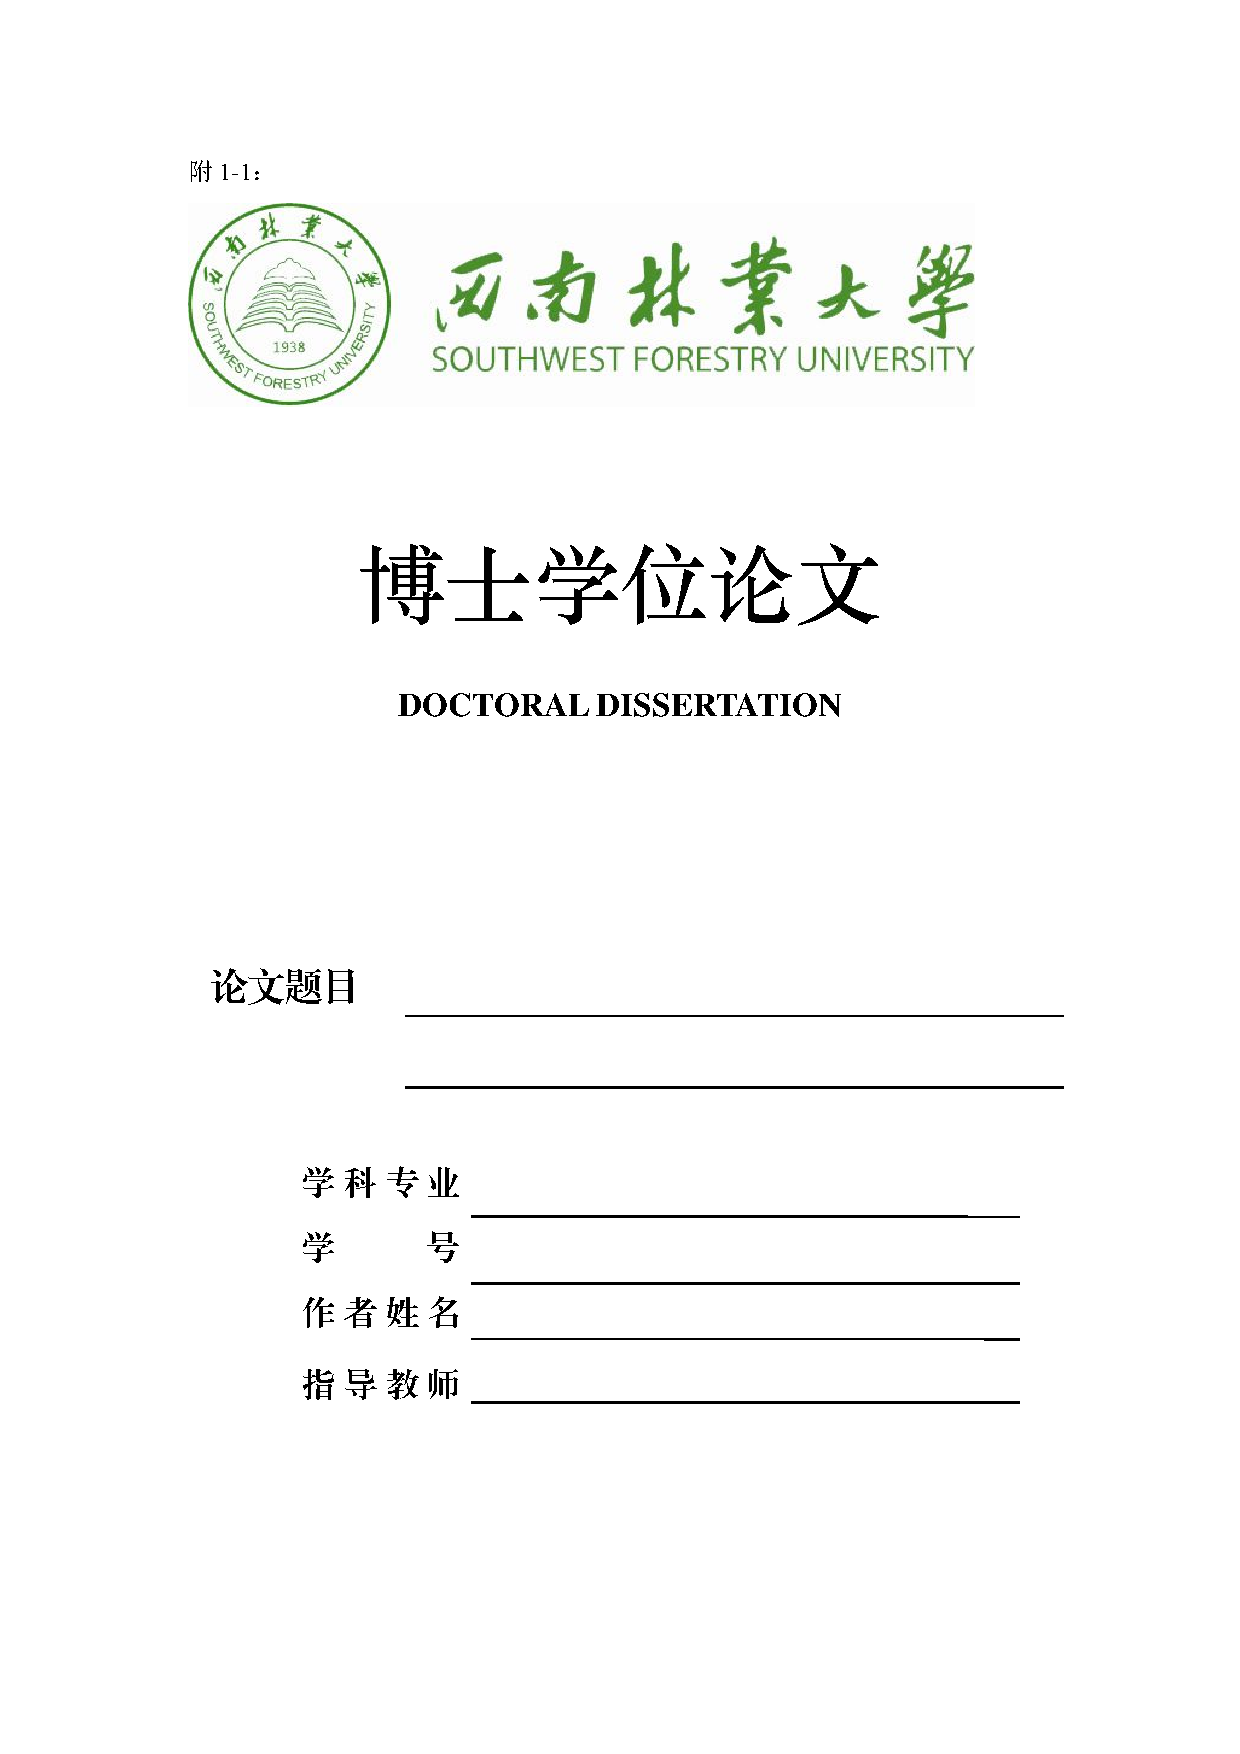
\includegraphics[width=\linewidth]{cover-phd}}
  \caption{博士论文封面\label{fig:cover-phd}}
\end{figure}

\begin{figure}[!ht]
  \centering\fbox{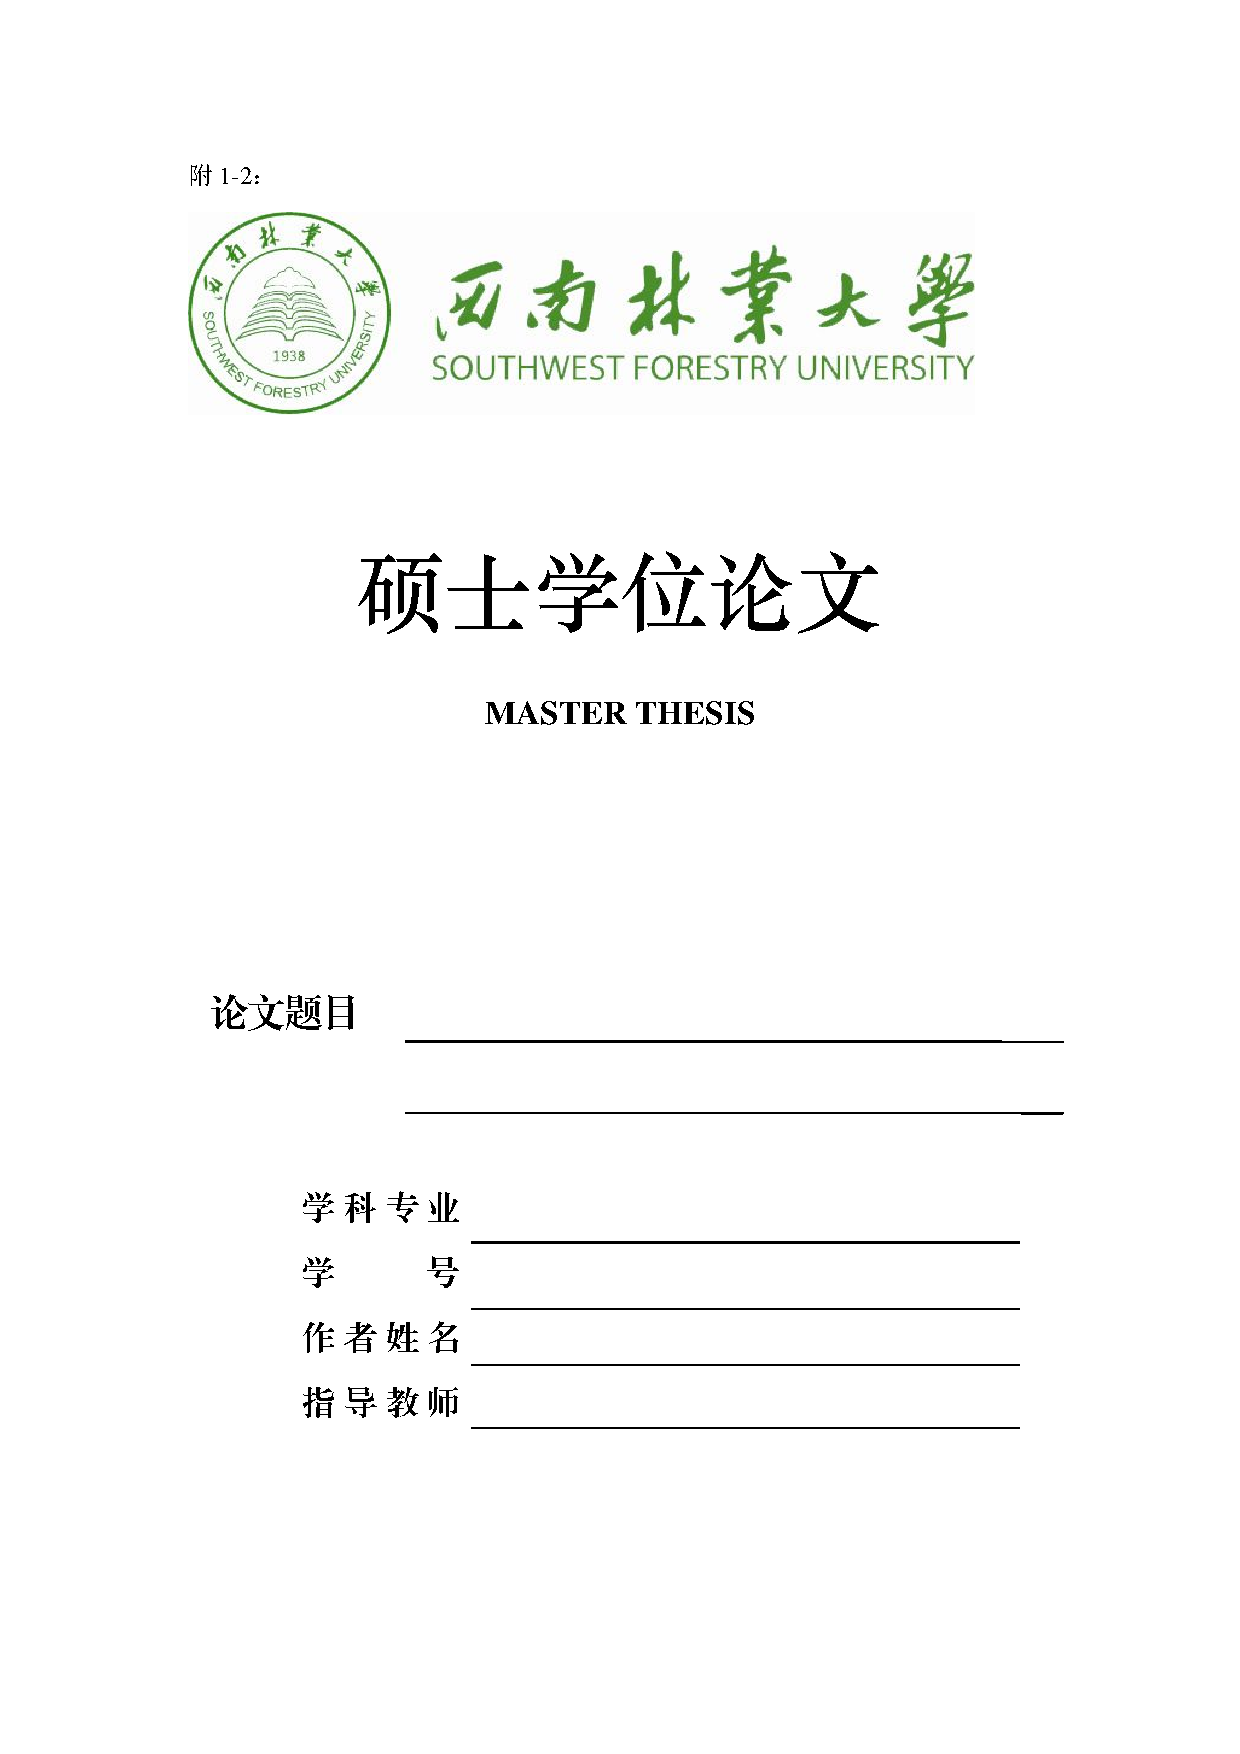
\includegraphics[width=\linewidth]{cover-msc}}
  \caption{硕士论文封面\label{fig:cover-msc}}
\end{figure}

\begin{figure}[!ht]
  \centering\fbox{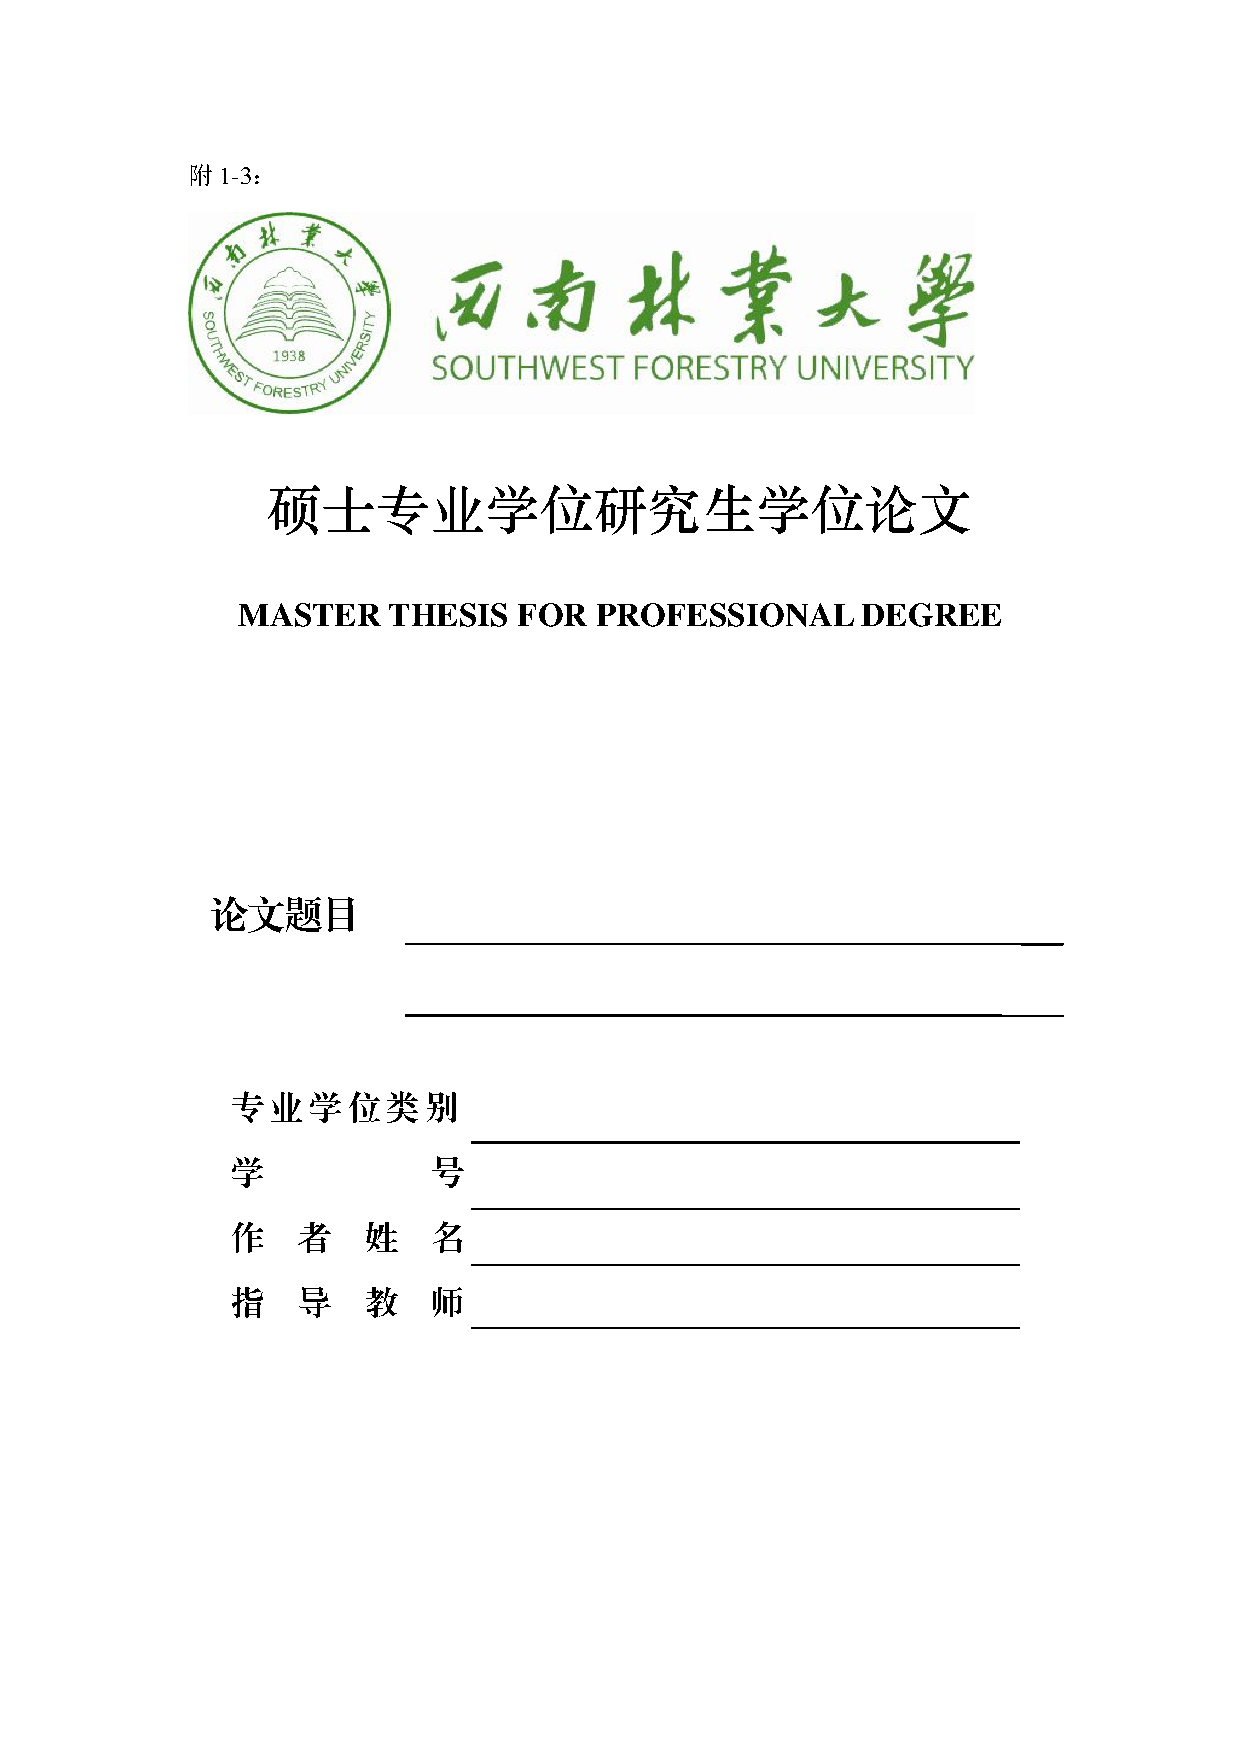
\includegraphics[width=\linewidth]{cover-msc2}}
  \caption{专业硕士论文封面\label{fig:cover-msc2}}
\end{figure}

\begin{figure}[!ht]
  \centering\fbox{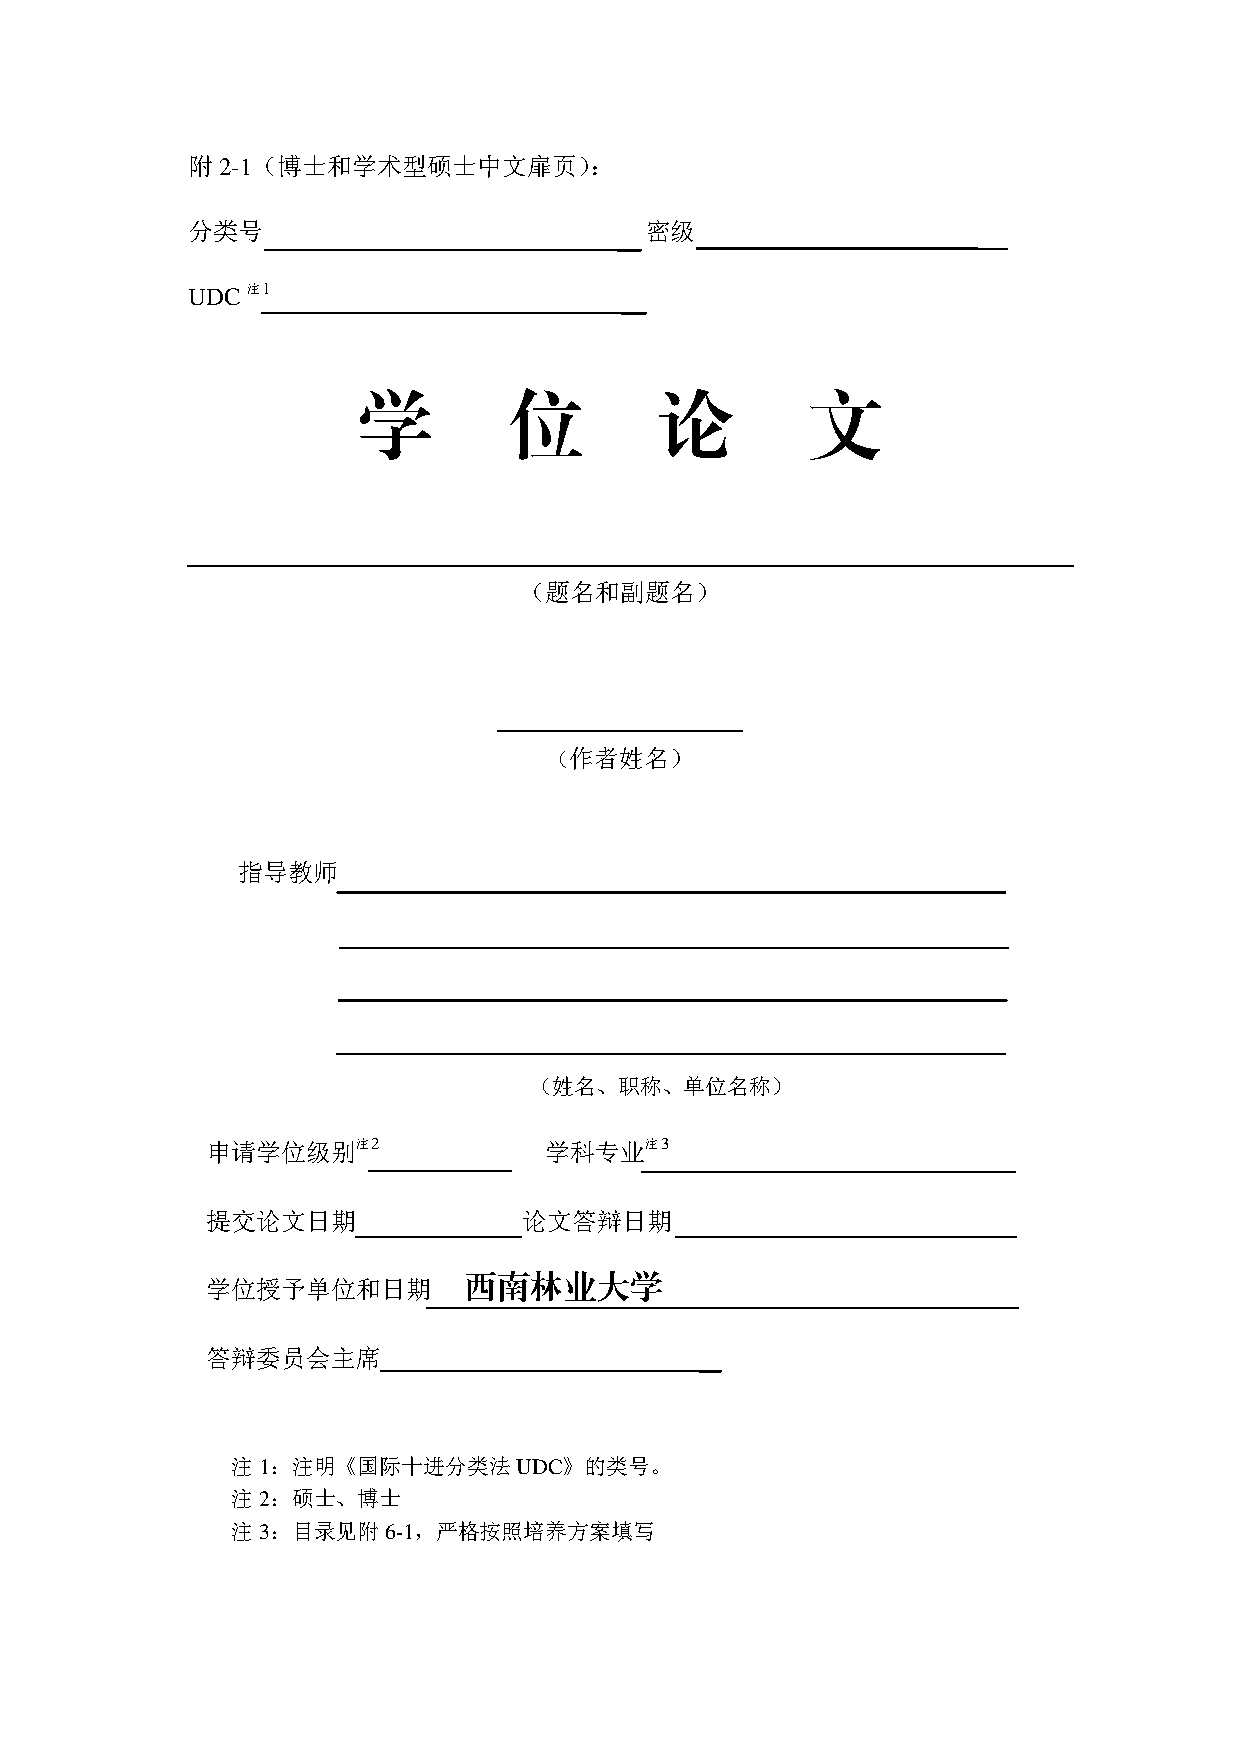
\includegraphics[width=\linewidth]{titlepage-phd}}
  \caption{博士和学术型硕士论文中文扉页\label{fig:titlepage-phd}}
\end{figure}

\begin{figure}[!ht]
  \centering\fbox{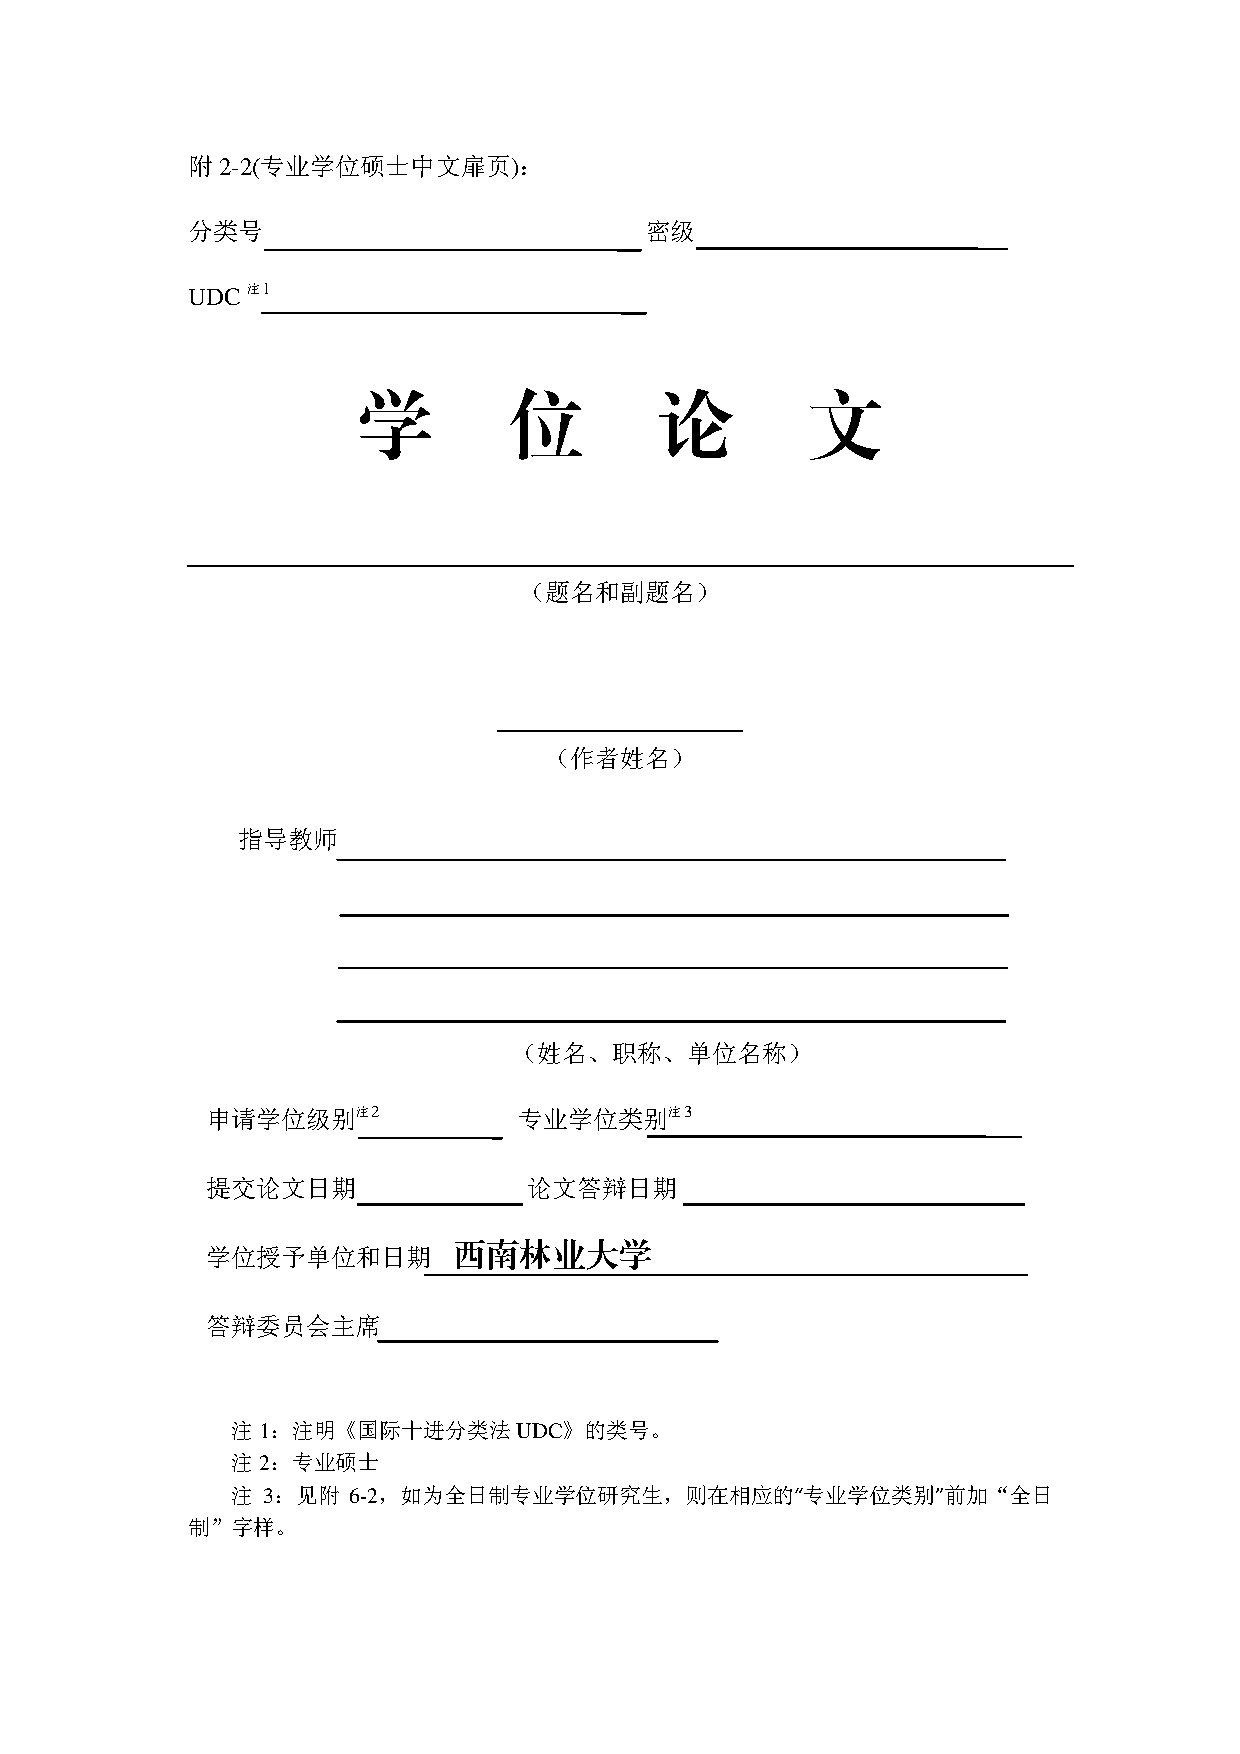
\includegraphics[width=\linewidth]{titlepage-msc2}}
  \caption{专业硕士论文中文扉页\label{fig:titlepage-msc2}}
\end{figure}

\begin{figure}[!ht]
  \centering
  \fbox{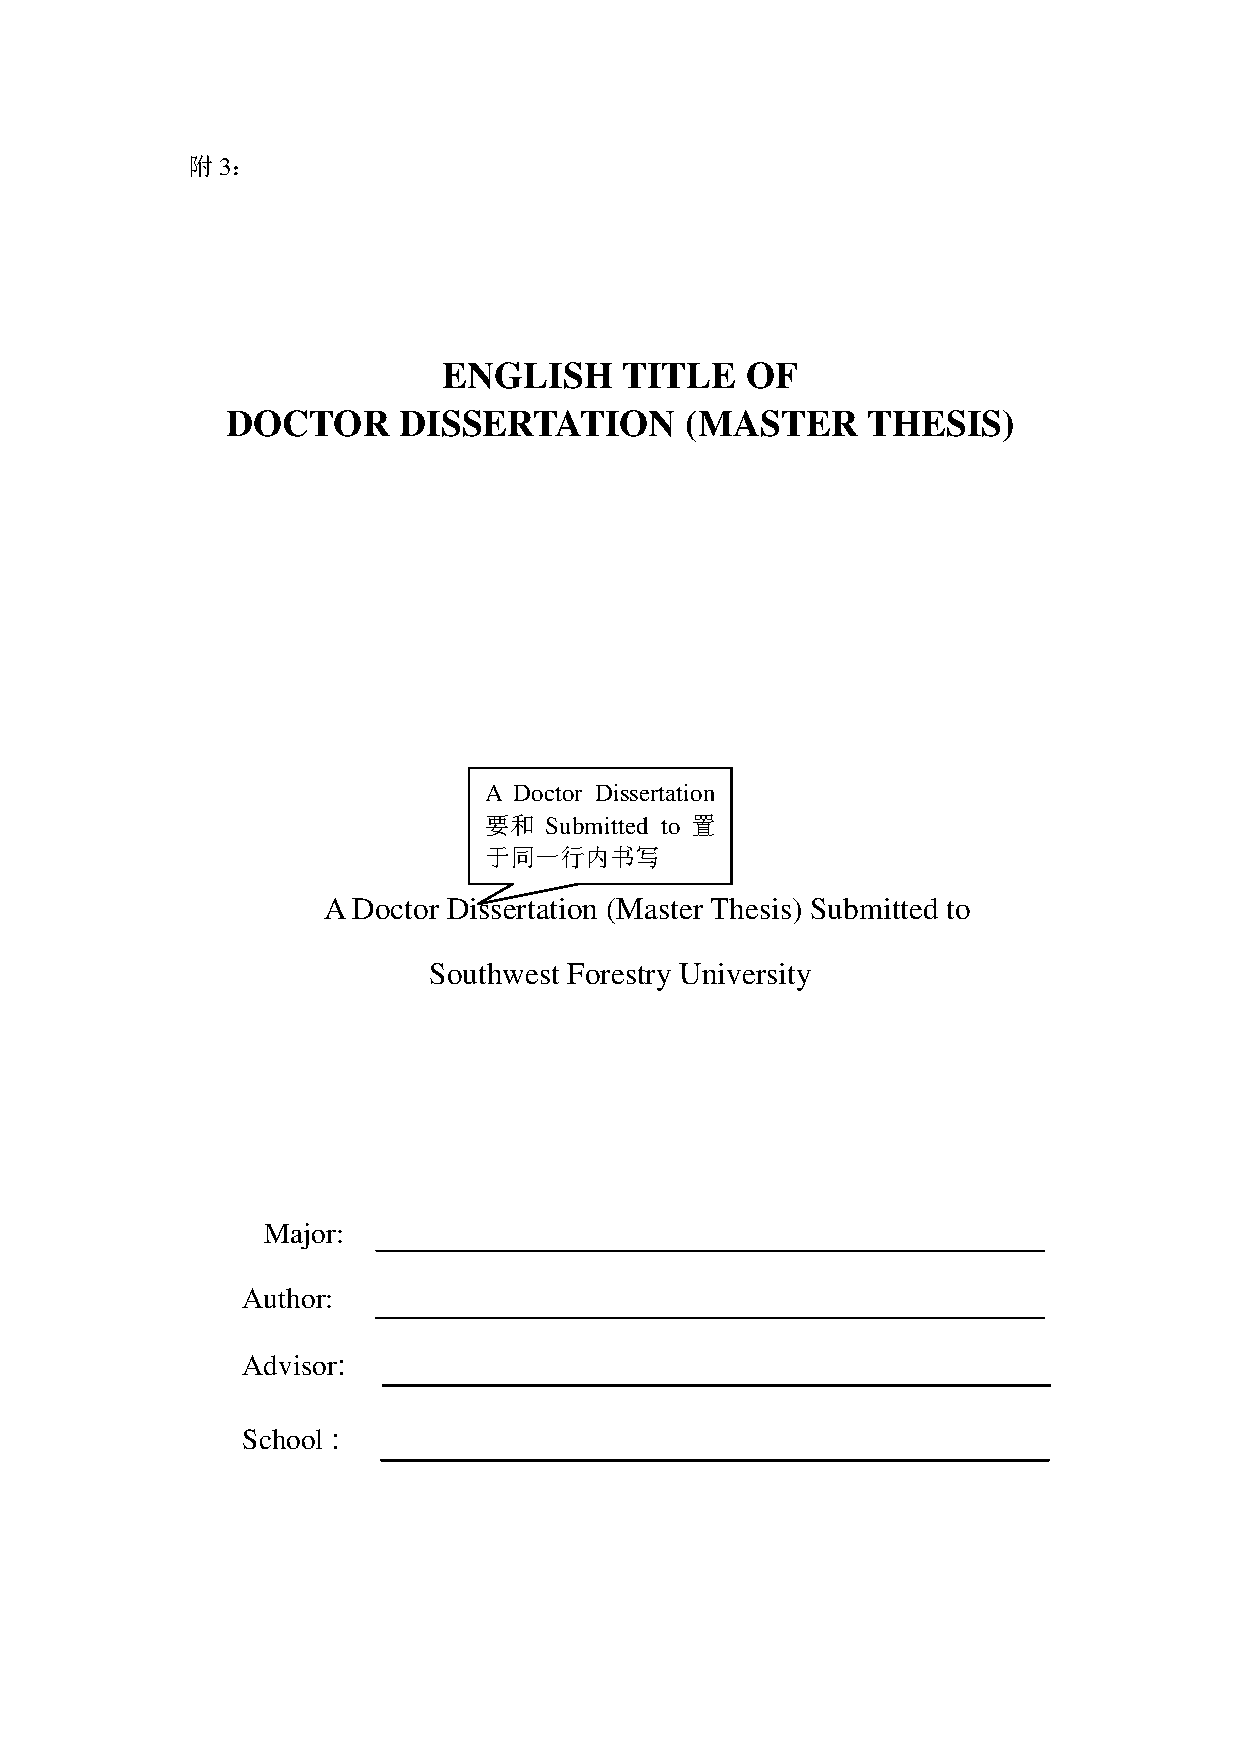
\includegraphics[width=\linewidth]{titlepage-en}}
  \caption{英文扉页\label{fig:titlepage-en}}
\end{figure}

\begin{figure}[!ht]
  \centering
  \fbox{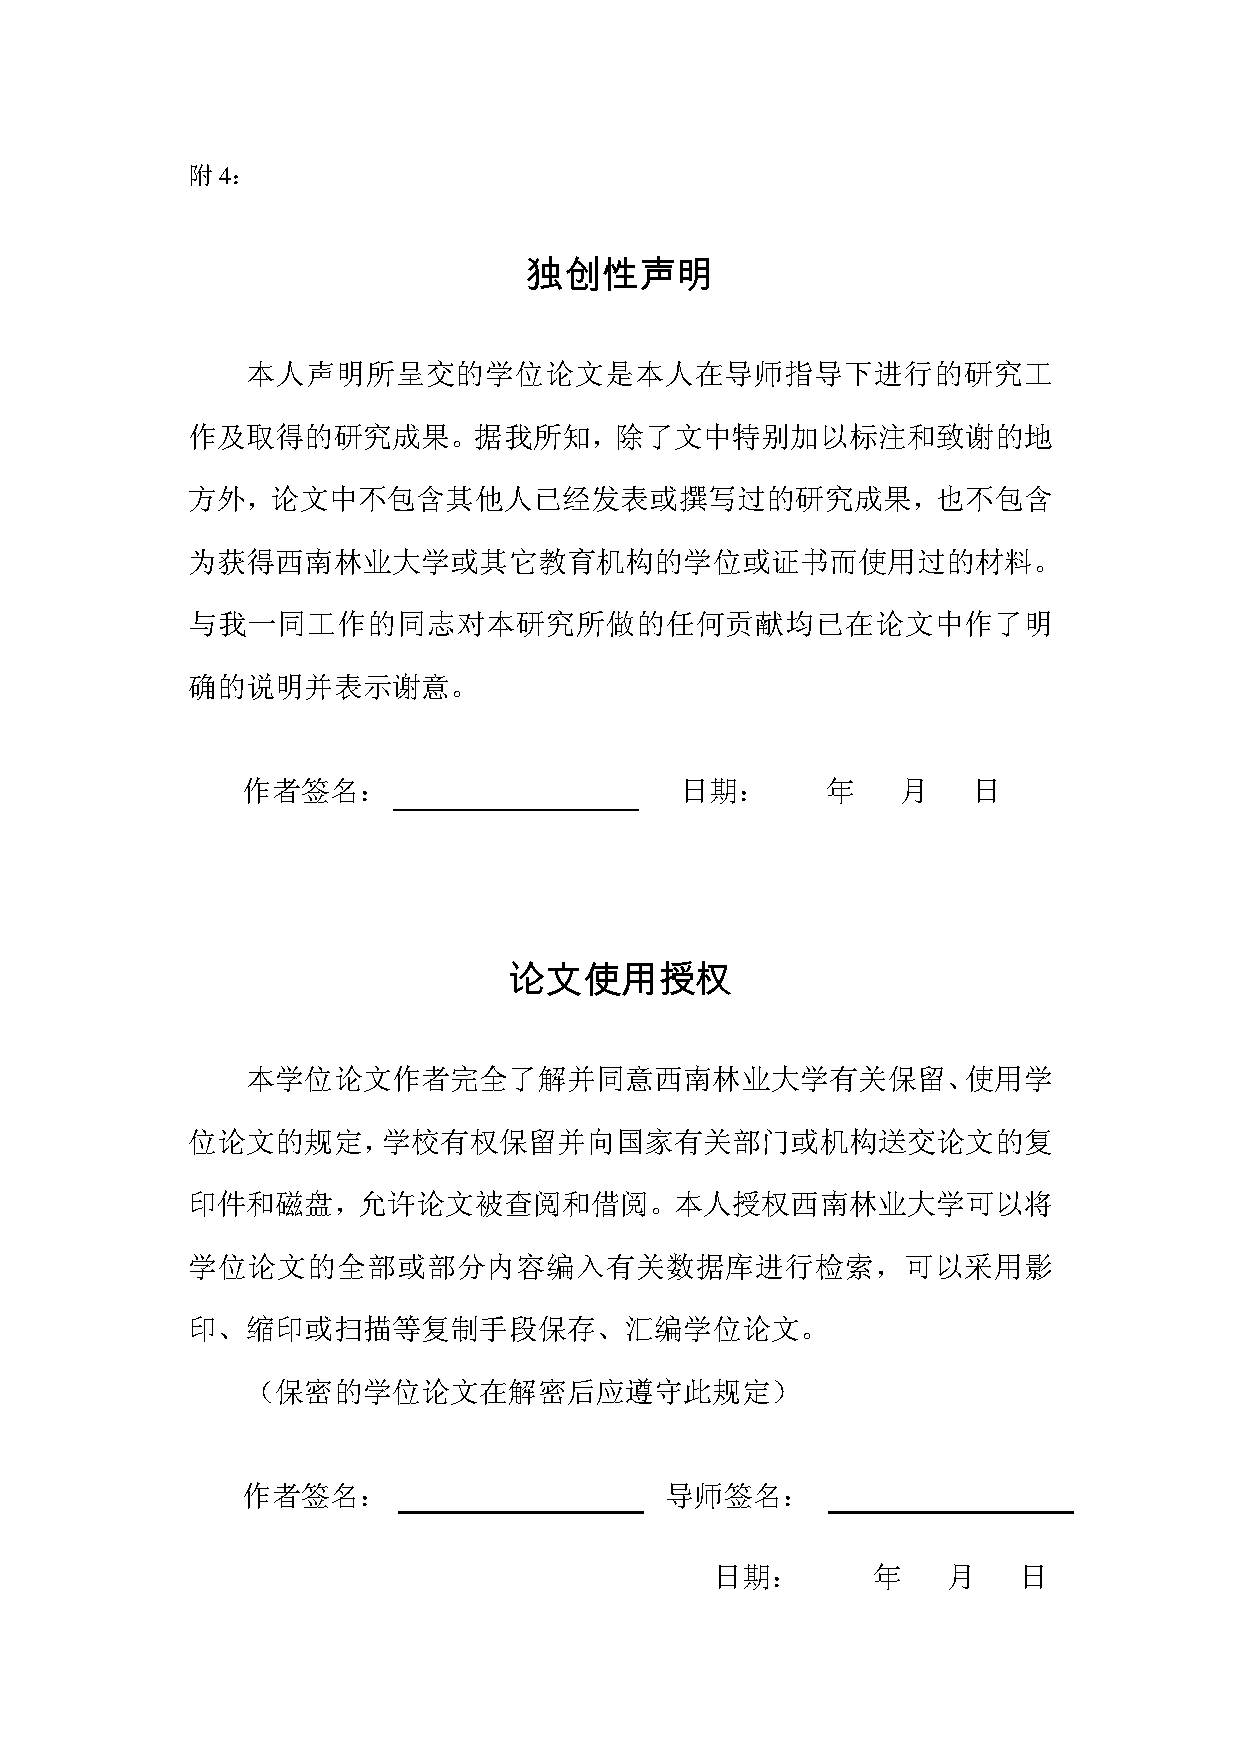
\includegraphics[width=\linewidth]{copyright}}
  \caption{独创性声明页\label{fig:copyright}}
\end{figure}

\begin{figure}[!ht]
  \centering
  \fbox{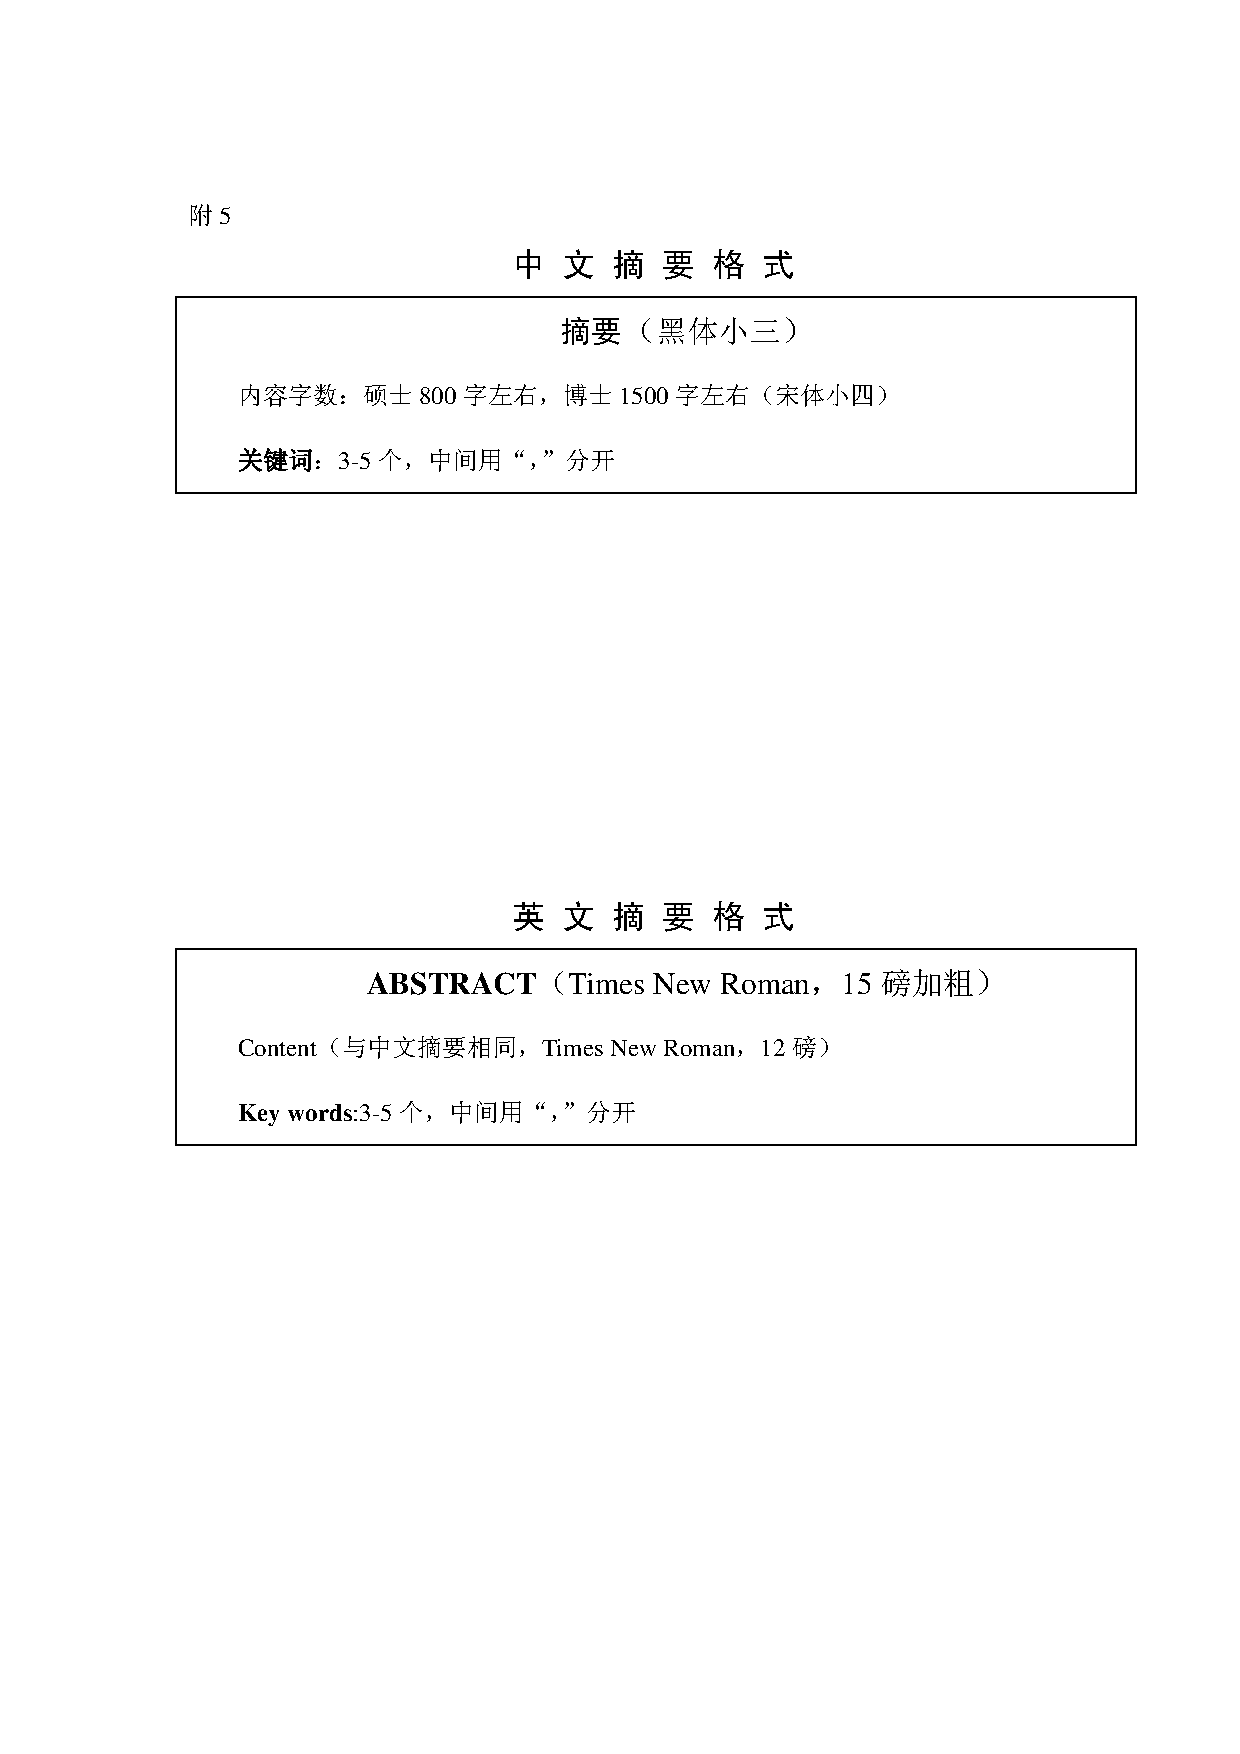
\includegraphics[width=\linewidth]{Abstract}}
  \caption{摘要格式\label{fig:Abstract}}
\end{figure}

%%% Local Variables:
%%% mode: latex
%%% TeX-master: "../example"
%%% End:


\chapter{与排版论文相关的软件清单}%
\footnotetext{这份清单是用如下命令获得的:\par
  \texttt{aptitude search '\~{}i "texlive|fonts|latexmk|pygments|emacs|fcitx|xterm|sawfish"' > pkg-list}}
\label{app:pkg}

\begin{enumerate}
\item emacs25 - GNU Emacs editor (with GTK+ GUI support)
\item emacs25-common-non-dfsg - GNU Emacs common non-DFSG items, including the core documentation
\item fcitx - Flexible Input Method Framework
\item fcitx-pinyin - Flexible Input Method Framework - classic Pinyin engine
\item fonts-noto - metapackage to pull in all Noto fonts
\item fonts-noto-cjk-extra - "No Tofu" font families with large Unicode coverage (CJK all weight)
\item fonts-arphic-ukai - "AR PL UKai" Chinese Unicode TrueType font collection Kaiti style
\item fonts-symbola - symbolic font providing emoji characters from Unicode 9.0
\item fonts-tlwg-purisa - Thai Purisa font (dependency package)
\item latexmk - Perl script for running LaTeX the correct number of times
\item sawfish - window manager for X11
\item sawfish-merlin-ugliness - More flexible functions for sawfish
\item texlive-bibtex-extra - TeX Live: BibTeX additional styles
\item texlive-extra-utils - TeX Live: TeX auxiliary programs
\item texlive-generic-extra - TeX Live: transitional dummy package
\item texlive-generic-recommended - TeX Live: transitional dummy package
\item texlive-lang-chinese - TeX Live: Chinese
\item texlive-lang-english - TeX Live: US and UK English
\item texlive-latex-recommended - TeX Live: LaTeX recommended packages
\item texlive-luatex - TeX Live: LuaTeX packages
\item texlive-xetex - TeX Live: XeTeX and packages
\item python-pygments - syntax highlighting package written in Python   
\item xterm - X terminal emulator
\end{enumerate}

\vspace{2ex}

注意,这是一个不完全的软件包列表。但是,在安装这些软件包时,其它一些被依赖的软件包会被自动
安装上。另外,Emacs的很多插件,比如\auctex{}, pdf-tools等,可以通过Emacs的插件管理模块来安装、
更新,在此没有列出。

%%% Local Variables:
%%% mode: latex
%%% TeX-master: "../tutorial"
%%% End:


\chapter{中文article模板}
\label{app:article}

\inputminted{latex}{article.tex}

\chapter{毕业论文模板}
\label{app:thesis}

\inputminted{latex}{thesis-template.tex}

\chapter{\texttt{swfuthesism.cls}文件}
\label{app:class}

\inputminted{latex}{swfuthesism.cls}

\chapter{\texttt{ref.bib}文件}
\label{app:bib}

\inputminted{bibtex}{ref.bib}


%%% tail pages
\doublespacing

\begin{authorInfo}
  某研究生,初从文,三年不中;后习武,校场发一矢,中鼓吏,逐之出;遂学医,有所成。自撰一良方,服之,卒。
\end{authorInfo}

\begin{advisorInfo}
  某教授,初从文,三年不中;后习武,校场发一矢,中鼓吏,逐之出;遂学医,有所成。自撰一良方,服之,卒。
\end{advisorInfo}

\publication{key1,key2,key3,key4,} %获得成果目录

\begin{acknowledgment}
  感谢美国计算机教授高德纳(Donald Ervin Knuth)编写的功能强大的排版软件\TeX{}。感谢美国计
  算机科学家莱斯利·兰波特(Leslie Lamport)教授为\TeX{}开发的简单易用的\LaTeX{}宏包。感谢本
  文作者能有如此多的闲功夫和好心情来饶有兴致地做这样一件不能当饭吃的事情。
\end{acknowledgment}

\end{document}
